\documentclass[12pt,a4paper,oneside]{report}
\usepackage{rotating}
\usepackage{pdflscape}
\usepackage{changepage}
\usepackage{algorithm}
\usepackage{algorithmic}
\usepackage{setspace}
\usepackage[framemethod=tikz]{mdframed}
\usepackage{tikz, xcolor, lipsum, colortbl}
\usepackage{amssymb}
\usepackage{multirow} 
\makeatletter
\mdfsetup{skipabove=\topskip,skipbelow=\topskip}
\tikzset{titreorange/.style =
    {draw=orange, line width=1.5pt, fill=white,
    rectangle, rounded corners, right,minimum height=2em}}
\newcommand{\titreencadre}{Titre}
\makeatletter
\mdfdefinestyle{encadresanstitrestyle}{
    linewidth=1.5pt,roundcorner=5pt,linecolor=orange,
    apptotikzsetting={\tikzset{mdfbackground/.append style ={
        fill=yellow!20}}},
    }
\newenvironment{encadresanstitre}{
    \begin{mdframed}[style=encadresanstitrestyle]
    }{\end{mdframed}}
\makeatother
\usepackage{pifont}
\usepackage[utf8]{inputenc}
\usepackage[arabic,main=french]{babel}
\usepackage[LFE,LAE,T1]{fontenc}
\renewcommand{\baselinestretch}{1.5}
\usepackage{appendix}
\usepackage{wrapfig}
\usepackage[backend=biber,style=ieee,citecounter=true]{biblatex}
\addbibresource{biblio.bib}
\setcounter{secnumdepth}{4}
\newcommand\tab[1][1cm]{\hspace*{#1}}
\usepackage[cyr]{aeguill}
\usepackage{graphicx}
\usepackage{adjustbox}
\usepackage{xspace}
\usepackage{wrapfig}
\usepackage{caption}
\usepackage{subcaption}
\usepackage{url}
\def\checkmark{\tikz\fill[scale=0.4](0,.35) -- (.25,0) -- (1,.7) -- (.25,.15) -- cycle;}
\usepackage[top=2cm, bottom=1.9cm, left=1.9cm, right=1.9cm]{geometry}
\usepackage{lettrine}
\usepackage{graphicx}
\usepackage{times}
\usepackage{geometry}
\usepackage[most]{tcolorbox}
\usepackage{pifont}
\usepackage{float} 
\usepackage{hyperref}
\usepackage{enumitem}
\setlist[enumerate,1]{label=\arabic*.}
\usepackage{textcomp}
\usepackage{array, makecell}
\usepackage{supertabular}
\usepackage{longtable}
\usepackage{tabularray}
\usepackage{fancyhdr}
\pagestyle{fancy}
\fancypagestyle{fancy}{
    \fancyhf{} 
    \fancyhead[L]{\nouppercase{\leftmark}} 
    % \fancyhead[R]{\nouppercase{\rightmark}}
    \fancyfoot[C]{\thepage}
    \renewcommand{\headrulewidth}{0.3pt}
}
\fancypagestyle{plain}{
  \fancyhf{}
  \fancyfoot[C]{\thepage}
  \renewcommand{\headrulewidth}{0pt}
} 
\usepackage[titles]{tocloft}
\usepackage{parskip}
\newlength\mylength
\renewcommand\cftchappresnum{\chaptername~}
\renewcommand\cftchapaftersnum{:}
\settowidth\mylength{\cftchappresnum\cftchapaftersnum\quad}
\addtolength\cftchapnumwidth{\mylength}
\usepackage{lmodern}
\usepackage[]{lipsum}
\newcommand\gauchedroite[2]{\noindent{}#1\hfill#2}
\usepackage[document]{ragged2e}
\justifying
\usepackage{fix-cm}
\usepackage{titlesec}
\renewcommand{\thesection}{\arabic{section}}
\renewcommand{\thesubsection}{\thesection.\arabic{subsection}}
\renewcommand{\thesubsubsection}{\thesubsection.\arabic{subsubsection}}
\titleformat{\section}{\normalfont\fontsize{16}{15}\bfseries}{\thesection.}{0.5em}{}
\titleformat{\subsection}{\normalfont\fontsize{14}{15}\bfseries}{\thesubsection.}{0.5em}{}
\titleformat{\subsubsection}{\normalfont\fontsize{12}{15}\bfseries}{\thesubsubsection.}{0.5em}{}
\titleformat{\chapter}{\normalfont\fontsize{16}{15}\bfseries}{\thechapter.}{0.5em}{}

\titlespacing*{\section}{0pt}{8pt}{8pt} 
\titlespacing*{\subsection}{4pt}{6pt}{6pt} 
\titlespacing*{\subsubsection}{6pt}{5pt}{5pt} 

\renewcommand{\cftsecaftersnum}{.}
\renewcommand{\cftsubsecaftersnum}{.}
\renewcommand{\cftsubsubsecaftersnum}{.}
\usepackage[Lenny]{fncychap}
\ChTitleVar{\Huge\bfseries}
\ChNameVar{\large\bfseries}
\ChNumVar{\fontsize{60}{62}\bfseries}
\ChTitleVar{\fontsize{20}{20}\bfseries}

\makeatletter
\def\@makechapterhead#1{%
  \vspace*{-20pt}
  {\parindent \z@ \raggedright \normalfont
    \ifnum \c@secnumdepth >\m@ne
      \if@mainmatter
        \DOCH
      \fi
    \fi
    \interlinepenalty\@M
    \if@mainmatter
      \DOTI{#1}%
    \else%
      \DOTIS{#1}%
    \fi
  }}
\makeatother
\usepackage{xhfill}
\usepackage{fdsymbol}
\usepackage{acronym} 
\usepackage{etoolbox}
\makeatletter
\let\oldcite\cite
\pretocmd{\listoffigures}{\def\cite{\ignorespaces\@gobble}}{}{}
\apptocmd{\listoffigures}{\let\cite\oldcite}{}{}
\pretocmd{\listoftables}{\def\cite{\ignorespaces\@gobble}}{}{}
\apptocmd{\listoftables}{\let\cite\oldcite}{}{}
\pretocmd{\tableofcontents}{\def\cite{\ignorespaces\@gobble}}{}{}
\apptocmd{\tableofcontents}{\let\cite\oldcite}{}{}
\makeatother
\begin{document}
    \pagenumbering{roman} 
    \pagestyle{plain}
        \enlargethispage{2cm}
\newgeometry{left=1.2cm, right=3.2cm, top=1.2cm, bottom=0.7cm}
\begin{titlepage}
\begin{table}[H]
    \centering
    \begin{tabular}{ccc}
        \begin{minipage}{.355\textwidth}
            \centering
            \fontsize{8}{10}\selectfont
            \textbf{République Tunisienne}\\
            \rule[0.5ex]{0.6in}{0.4pt} \hspace{0.3cm} $\medblackdiamond$ \hspace{0.3cm} \rule[0.5ex]{0.6in}{0.4pt}\\
            \textbf{Ministère de l’Enseignement Supérieur}\\
            \textbf{et de la Recherche Scientifique}\\
            \textbf{Université de Tunis}\\
            \rule[0.5ex]{0.6in}{0.4pt} \hspace{0.3cm} $\medblackdiamond$ \hspace{0.3cm} \rule[0.5ex]{0.6in}{0.4pt}\\
            \textbf{ École Nationale Supérieure}\\
            \textbf{ d’Ingénieurs de Tunis}
        \end{minipage}
        &
        \begin{minipage}{.42\textwidth}
            \centering
            \fontsize{9}{8}\selectfont
           \textbf{\textsf{RAPPORT DE PROJET DE FIN D’ETUDES} }
        \end{minipage}
        &
        \begin{minipage}{.27\textwidth}
            \raggedleft
            
\includegraphics[width=0.9\textwidth]{pages/page-de-garde/img/ensit.PNG}\\
            \vspace{0.5cm}
            \fontsize{8}{10}\selectfont
            \textbf{Code: GSP-RP-04-00}\\
            \textbf{Date de création: 16-06-2023}
        \end{minipage}
    \end{tabular}
\end{table}
\vspace{-1.4cm}
\makebox[1.12\textwidth]{\textcolor{red}\hrulefill}
 \\ \vspace{0.2cm}
\noindent
\parbox{0.4\textwidth}{
    \centering
    
\includegraphics[width=0.14\textwidth]{pages/page-de-garde/img/logo-d.PNG} \\
    \fontsize{10}{9}\selectfont
    \textbf{Département Génie Informatique}
}
\hfill 
\parbox{0.7\textwidth}{
    \vspace{-1.5cm}
    \raggedleft
    \textbf{\small N°: Ing-GInfo-28-2025}
}
\vspace{0.1cm}
\begin{adjustwidth}{1.6cm}{0cm}
 \begin{center}
        \textbf{\Large RAPPORT DE PROJET DE FIN D’ETUDES}\\
        \vspace{0.5cm}
        \textbf{\small \fontsize{12}{6}\selectfont Présenté en vue de l’obtention du}\\
        \vspace{0.2cm}
        \textbf{\small \fontsize{12}{6}\selectfont Diplôme National d’Ingénieur en Génie Informatique}\\
        \vspace{0.2cm}
        \textbf{\small \fontsize{12}{6}\selectfont Spécialité: Nouvelles technologies et sécurité (NTS)}\\
        \vspace{0.5cm}
        \textbf{\small \fontsize{12}{6}\selectfont Par: CHERNI Rihab } \\
        \vspace{-0.6cm}
        \begin{adjustwidth}{-1cm}{0cm}
            \begin{center}
                \setlength{\fboxsep}{10pt} 
                \setlength{\fboxrule}{4pt} 
                \fbox{
                    \begin{minipage}{\textwidth}
                        \centering \fontsize{17}{16}\selectfont\textbf{Développement d'une application web "AutoTest": Solution pour automatiser les tests fonctionnels, les analyses de sécurité et l’audit de référencement naturel}\\
                    \end{minipage}
                }\\
            \end{center}
        \end{adjustwidth}
         \Large \fontsize{12}{12}\selectfont Réalisé au sein \textbf{de ADDINN Tunis} \\
         
\includegraphics[width=6cm]{pages/page-de-garde/img/logo.png}\\
         \textit{\Large \fontsize{12}{12}\selectfont  Soutenu le \textbf{30 juin 2025}, devant le jury composé de:} \\
        \vspace{-0.5cm}
        \begin{center}
            \renewcommand{\arraystretch}{1.5} 
            \begin{tabular}{p{0.5\textwidth}p{0.5\textwidth}}
                    \textbf{Président:} & M. BOULARES Mehrez\\
                    
                    \textbf{Rapporteur:} & Mme. GHRAIRI Salsabil\\
                    
                    \textbf{Encadrant universitaire:} & Mme ELOUEDI Ines\\
                    
                    \textbf{Encadrant industriel:} & M. NACHMI Omar\\
                \end{tabular}
        \end{center}
        \vspace{0.15cm}
        \textbf{\fontsize{13}{12} \textsf{Année Universitaire 2024-2025}} \\
        \vspace{-0.3cm}
\end{center}
\end{adjustwidth}
\begin{center}
    % \makebox[1.15\textwidth]{\hspace{-0.8cm}\textcolor{gray}\hrulefill}
    \makebox[1.12\textwidth]{\textcolor{red}\hrulefill}
    \vspace{-0.4cm}
    \begin{tiny}
         \begin{table}[H]
            \begin{tabular}{p{.33\textwidth}p{.3\textwidth}p{.3\textwidth}}
                \begin{minipage}{.4\textwidth}
                    \fontsize{9}{6}\selectfont 5, Avenue Taha Hussein–Tunis 
                \end{minipage} 
                 &
                \begin{minipage}{.3\textwidth}
                \centering
                     \fontsize{9}{6}\selectfont
                        \begin{tabular}{cc}
                           \href{https://www.ensit.tn/}{\color{blue}\underline{www.ensit.tn/}}
                         \end{tabular}
                 \end{minipage}
                 &
               \begin{minipage}{.4\textwidth}
                    \raggedleft
                    \small \fontsize{9}{6}\selectfont       Tel.: (+216)71 49 68 80;71 49 402   
                \end{minipage}\\
                \begin{minipage}{.33\textwidth}\fontsize{9}{6}\selectfont B. P. 56, Bab Menara 1008 \end{minipage}& &
                \begin{minipage}{.4\textwidth}
                    \raggedleft
                \small \fontsize{9}{6}\selectfont
                   Fax: (+216) 71 39 11 66  
                \end{minipage}
            \end{tabular}
        \end{table} 
    \end{tiny} 
    \end{center}
\end{titlepage}
\restoregeometry
 \newpage
        \begin{center}
    \textbf{\textit{\Huge Dédicaces}}\\
\end{center}
\vspace{1.5cm}
\begin{center}
    \textit{Je dédie ce projet à mes parents, mes sœurs, mes amis, ainsi qu’à tous mes collègues et professeurs. Leur soutien m’a beaucoup aidé et m’a donné la force d’avancer tout au long de ce parcours.}\\
    \vspace{0.9cm}
    \textit{À mes parents, pour leur amour, leur patience et leur courage, surtout dans les moments difficiles. Grâce à eux, j’ai pu recevoir une bonne éducation et avancer vers mes objectifs.}\\
    \vspace{0.9cm}    
    \textit{À mes deux sœurs, Arij et Rania, pour leur présence, leurs paroles gentilles et leurs encouragements qui m’ont toujours réconforté.}\\
    \vspace{0.9cm}
    \textit{À mes amis, qui sont comme une seconde famille. Merci pour leur aide, leur bonne humeur et leur soutien tout au long de ce chemin.}\\
    \vspace{0.9cm}
    \textit{Et à toutes les personnes qui m’ont aidé, de près ou de loin, un grand merci du fond du cœur.}\\
\end{center}
 \newpage
        \begin{center}
    \textbf{\textit{\Huge Remerciements}}\\
\end{center}
\vspace{1cm}
\begin{center}
    \textit{Je tiens à exprimer ma profonde gratitude à toutes les personnes qui, de près ou de loin, ont contribué à la réussite de ce projet de fin d’études et à l’enrichissement de cette expérience.}
    
    \textit{Tout d’abord, je remercie Mme Ines Elouedi, mon encadrante universitaire, pour son suivi attentif, ses précieux conseils et son accompagnement tout au long de ce projet. Sa bienveillance et son expertise ont été d’une aide précieuse pour mener ce travail à bien.}
    
    \textit{Je tiens également à exprimer ma reconnaissance à monsieur Omar Nachmi, mon encadrant industriel au sein de ADDINN Tunis, pour sa disponibilité, son encadrement et ses orientations pertinentes, qui m’ont permis de mener ce projet à bien dans un cadre professionnel enrichissant.}
    
    \textit{Mes sincères remerciements vont aussi à toute l’équipe de ADDINN Tunis pour leur accueil chaleureux et leur esprit collaboratif, qui ont rendu cette expérience aussi formatrice qu’agréable.}
    
    \textit{Je remercie également les membres du jury pour l’intérêt qu’ils portent à mon travail et pour leurs précieuses évaluations.}
    
    \textit{Je suis reconnaissant envers tous mes enseignants de l'École Nationale Supérieure d'Ingénieurs de Tunis (ENSIT) pour leur engagement et leur contribution à ma formation.}
    
    \textit{Enfin, je remercie ma famille et mes amis pour leur soutien inconditionnel, leurs encouragements constants et leur présence précieuse tout au long de cette aventure.}

    \textit{\textbf{Un grand merci à tous.}}

\end{center}
 \newpage
    \pagestyle{fancy}
        \addtocontents{toc}{\vspace{-0pt}}
        \begin{spacing}{1.1}
            \tableofcontents            
            \addtocontents{lof}{\vspace{-60pt}}
            \listoffigures
            \addtocontents{lot}{\vspace{-60pt}}
            \listoftables  \newpage
        \end{spacing}
        \thispagestyle{empty}
        \pagenumbering{arabic} 
    \setcounter{page}{1}
    \pagestyle{plain}
        \addtocontents{toc}{\vspace{-60pt}}
        \chapter*{\begin{center} \huge \vspace{-3.5cm} \textbf{Introduction générale} \end{center}}
\addcontentsline{toc}{chapter}{Introduction générale}
\vspace{-2.5cm}
    \begin{justify}
        La sécurité des applications web constitue un enjeu majeur face à l’augmentation des cyberattaques, dont les vulnérabilités peuvent entraîner la perte de données sensibles. Cependant, les méthodes traditionnelles de détection de ces failles restent souvent manuelles, lentes, limitées, coûteuses et sujettes aux erreurs humaines. Dans ce contexte, les tests de pénétration jouent un rôle crucial en permettant d’identifier les failles avant qu’elles ne soient exploitées par des attaquants.
        
        En parallèle, les tests fonctionnels vérifient que les fonctionnalités d’une application respectent les spécifications et fonctionnent correctement dans divers scénarios. Ils permettent de s’assurer que les interactions, les flux de travail, les formulaires, les boutons, et les diverses actions proposées à l’utilisateur se comportent comme prévu. Bien que souvent réalisés manuellement, leur automatisation permet un gain de temps, une meilleure couverture des tests et une réduction des erreurs humaines. Cela facilite la détection rapide des dysfonctionnements, améliore la qualité globale de l’application et assure une expérience utilisateur fluide. Ces tests sont essentiels pour garantir la robustesse du produit, prévenir les bugs et renforcer la confiance des utilisateurs.   
        
        De plus, l’optimisation du référencement naturel (audit SEO) est essentielle pour évaluer et améliorer la visibilité d’un site ou d’une application web sur les moteurs de recherche. Elle permet d’identifier les points forts, les faiblesses et les axes d’amélioration du positionnement. L’automatisation de ces tests permet de détecter rapidement ces problèmes et d’optimiser la qualité technique globale.
    
        L’objectif de ce projet est de concevoir et développer une application web pour automatiser :
        \begin{itemize}[left=-0.1cm, label=$\bullet$]
            \item \textbf{Les tests de pénétration :} Intégrer divers outils de sécurité afin d'améliorer la détection des vulnérabilités, qu’elles soient similaires ou complémentaires, dans le cadre des tests d'intrusion. Cela inclut la gestion de la progression des scans, la comparaison et la corrélation des vulnérabilités, la fusion des résultats en un rapport final unifié, la surveillance en temps réel des vulnérabilités détectées, l’implémentation d’une authentification dynamique pour simuler des scénarios d’attaque sur des applications protégées par des pages de connexion, ainsi que la validation automatique des faux positifs.
            \item \textbf{Les tests fonctionnels :} Automatiser les tests pour vérifier que les fonctionnalités principales des applications web fonctionnent correctement et tester les interfaces utilisateur pour s'assurer de leur conformité avec les attentes.
            \item \textbf{Les tests SEO :} Identifier automatiquement les erreurs techniques pouvant affecter le référencement naturel, telles que les liens cassés, les redirections défaillantes, l’absence ou la mauvaise configuration des balises essentielles, ainsi qu’un temps de chargement excessif, qui peuvent nuire à l’indexation et à la performance globale. Fournir ensuite des recommandations pour améliorer la visibilité de l’application sur les moteurs de recherche.
        \end{itemize}
    
        Le rapport présente les étapes du projet, structuré comme suit :
        \begin{itemize}[left=-0.1cm, label=$\bullet$]
            \item \textbf{Chapitre 1 : "Cadre général du projet" :} Contexte général du projet, présentation de la société d’accueil, analyse des solutions existantes sur le marché et la méthodologie de travail.
            \item \textbf{Chapitre 2 : "Sprint 0 - Étude préliminaire" :} Analyse des besoins fonctionnels et non fonctionnels, découpage du projet et élaboration du backlog produit. Présentation exhaustive des outils et technologies adoptés lors de l’implémentation, ainsi que de l’architecture de l’application.
            \item \textbf{Chapitre 2 : "Analyse et planification du projet" :} Analyse des besoins fonctionnels et non fonctionnels, découpage du projet et élaboration du backlog produit, ainsi que présentation détaillée des outils et technologies utilisés lors de l’implémentation et de l’architecture de l’application.
            \item \textbf{Chapitre 3 : "Sprint 1 -  Automatisation des tests de sécurité et amélioration des fonctionnalités de base.}
            \item \textbf{Chapitre 4 : "Sprint 2 - Automatisation des tests fonctionnels et SEO, génération de rapports et déploiement.".}
        \end{itemize}
        
        Enfin, une conclusion générale résumera les résultats réalisés et proposera des perspectives d’amélioration, tout en énumérant les compétences que nous avons acquises durant ce stage.
    \end{justify}
    
    
 \newpage
    \pagestyle{fancy}
        \chapter{Cadre général du projet}
\renewcommand{\thesection}{\arabic{section}}
\vspace{-1cm}
\begin{justify}
    \section*{\texorpdfstring{Introduction}{Introduction}}
    \addcontentsline{toc}{chapter}{\textbf{Introduction}}
    Ce premier chapitre présente le contexte général du projet et l’organisme d’accueil, en analysant et en critiquant les solutions existantes ainsi que l’état actuel de la première version l’application, tout en mettant en évidence leurs limites afin de justifier la nécessité d’une nouvelle approche. Il expose également la solution proposée ainsi que la méthodologie adoptée pour sa mise en œuvre.
    \section{\texorpdfstring{Contexte général du projet}{Contexte général du projet}}
    Dans le cadre de l'obtention du diplôme national d'ingénieur en génie informatique, spécialité \ac{NTS}, à l'\ac{ENSIT}, une opportunité a été offerte pour réaliser un projet de fin d'études au sein de la société ADDINN Tunisie, au sein de l'équipe \ac{QA}, pour une durée de quatre mois, durant l'année universitaire 2024/2025.
    \section{Présentation de l’organisme d’accueil}
    Dans cette section, nous présentons l’organisme d’accueil en abordant son histoire, ses valeurs, ainsi que ses partenariats qui contribuent à son succès et à son développement.
\subsection{\texorpdfstring{Aperçu général d'Addinn}{Aperçu général d'Addinn}}
    \begin{minipage}{.6\textwidth}
        \justifying
        Addinn est un cabinet de conseil en transformation digitale spécialisé dans l’accompagnement des entreprises pour définir leur stratégie et mettre en œuvre leurs projets technologiques grâce à un écosystème innovant et complémentaire permet de relever les défis numérique avec succès\cite{Addinn}.\\
    \end{minipage}
    \begin{minipage}{.4\textwidth}
        \vspace{-2.1cm}
        \begin{figure}[H]
            \centering
            
\includegraphics[width=\linewidth]{pages/page-de-garde/img/logo.png}
            \caption{\centering Logo d'\acs{ADDINN}\protect{\cite{Addinn}}}
            \label{fig:logo-ADDINN}
        \end{figure}
    \end{minipage}
\vspace{-0.8cm}
\subsection{Fondements de la Société\cite{apropos}}
    \acs{ADDINN} a pour mission de créer de la valeur à chaque étape de la réflexion à la mise en œuvre et au déploiement des projets \acs{IT}. Son engagement en faveur de l’innovation se reflète dans sa devise "\textbf{ADD} VALUE BY \textbf{INN}OVATION", illustrant sa volonté d’apporter une réelle valeur ajoutée à ses clients. Grâce à son approche novatrice et son expertise, l'entreprise aide à relever les défis avec agilité et efficacité, garantissant ainsi une transformation réussie et durable.\\
    Le tableau~\ref{tab:objectifs} présente les objectifs et les valeurs qui orientent l’approche d’ADDINN:
    \begin{table}[H]
        \centering
        \caption{Synthèse des objectifs stratégiques et des valeurs portées par ADDINN}
        \renewcommand{\arraystretch}{1.5}
        \begin{tabular}{|c|c|}
            \hline
          \textbf{ Objectifs d’ADDINN }  & \textbf{Valeurs d’ADDINN}\\ \hline
            \begin{minipage}{.48\textwidth}
                \vspace{0.15cm}
                 \begin{justify}
                    \begin{itemize}[label=$\bullet$,left=-0.1cm]
                        \item Optimiser les flux de travail afin de les rendre plus rapides et simples.
                        \item Développer des systèmes et des solutions plus efficaces.
                        \item Améliorer l'expérience de clients et accroître l'avantage concurrentiel de l'entité.
                    \end{itemize}
                \end{justify}
                \vspace{0.15cm}
            \end{minipage}
              & 
            \begin{minipage}{.48\textwidth}
                \vspace{0.15cm}
                 \begin{justify}
                    \begin{itemize}[label=$\bullet$,left=-0.1cm]
                        \item \textbf{Innovation}: Pousser plus loin les idées grâce à la recherche et au développement.
                        \item \textbf{Agilité}: Reposer sur la flexibilité et la collaboration comme principes fondamentaux.
                        \item \textbf{Excellence}: Viser la qualité à travers une approche structurée et optimisée.
                    \end{itemize}
                \end{justify}
                \vspace{0.15cm}
            \end{minipage} \\\hline
        \end{tabular}
        \label{tab:objectifs}
    \end{table}
    \vspace{-0.6cm}
\subsection{Fiche de présentation d'ADDINN}
        Le table ~\ref{tab:infoADD} fournit un aperçu détaillé de l'organisme d'accueil.
        \begin{table}[H]
            \caption{\centering Fiche de présentation de la société d'ADDINN \cite{Addinn}\cite{apropos}} 
            \centering
            \renewcommand{\arraystretch}{1.5}
            \begin{tabular}{|p{2.3cm}|p{14cm}|}
                \hline
                    \textbf{Nom} & \textbf{ADDINN}\\
                \hline
                    \textbf{Type} & Société de conseil en transformation digitale\\
                \hline
                    \textbf{Adresses} & 
                        \begin{minipage}{14cm}
                            \begin{justify}
                                \vspace{0.15cm} 
                                \begin{itemize}[left=-0.1cm,label=$\bullet$]
                                    \item \textbf{ADDINN Groupe (France):} 121 Avenue Champs-Elysées Paris 75008.
                                    \item \textbf{ADDINN Tunis:} Immeuble Etraton, Rue Khadija Ben Arfa, Centre Urbain Nord 1082.
                                    \item \textbf{ADDINN Sousse:} Rue Hedi Nouira Akouda Sousse 4022.
                                    \item \textbf{ADDINN Tozeur:} Immeuble Akouri, 2ème étage, rue 2 Mars, Tozeur.
                                    \item \textbf{ADDINN Africa (Congo Brazzaville):} N°3 Allée des Manguiers Beach Centre-ville – Brazzaville.
                                \end{itemize}    
                                \vspace{0.15cm}        
                            \end{justify}
                        \end{minipage}\\
                \hline
                    \textbf{Chiffres Clés} & 
                        \begin{minipage}{14cm}
                            \vspace{0.15cm} 
                            \begin{itemize}[left=-0.1cm,label=$\bullet$]
                                \item Plus de 11 ans d’expérience en consulting IT.  
                                \item Plus de 100 consultants et ingénieurs qualifiés.  
                                \item 90\% des projets gérés en Agile/Scrum.  
                                \item Plus de 40 experts certifiés.  
                            \end{itemize}
                        \end{minipage}\\
                \hline
                    \textbf{Domaines d'expertise} & Conseil en stratégie, conseil en transformation digitale, développement IT et solutions numériques. \\
                \hline 
                    \textbf{Email} & 
                        contact@addinn.com et sales@addinn.com \\
                \hline
                    \textbf{Site web} & \url{https://addinn-group.com/}\\
                \hline
            \end{tabular}
            \label{tab:infoADD}
        \end{table} 
    \vspace{-0.5cm}
    \subsection{Histoire de croissance d’ADDINN et présence internationale\cite{apropos}}
        L’histoire d’ADDINN débute en 2012, avec la rencontre de deux amis ambitieux souhaitant prendre part à la révolution digitale. Plus d’une décennie d’efforts, d’innovations technologiques et de stratégie d’expansion a permis à l’entreprise de franchir ses frontières d’origine.
        \begin{minipage}{.55\textwidth}
            \begin{justify}
                Aujourd’hui, ADDINN Group s’impose comme un acteur clé du marché euro-méditerranéen et africain. Avec son siège social à Paris, le groupe a étendu ses activités en créant 3 filiales en Tunisie, en Mauritanie et au Congo-Brazzaville , comme le montre la figure~\ref{fig:presence_addinn}.
                
                Grâce à des partenariats solides, ADDINN maintient des relations privilégiées avec ses clients au Gabon, en République Démocratique du Congo et en Belgique, consolidant ainsi son expansion à l'international.  
                
                Le tableau~\ref{tab:etapes_addinn} résume les étapes clés de cette croissance.
            \end{justify}
        \end{minipage}
        \hspace{0.1cm}
        \begin{minipage}{.45\textwidth}
            \vspace{-1cm}
            \begin{figure}[H]
                \centering
                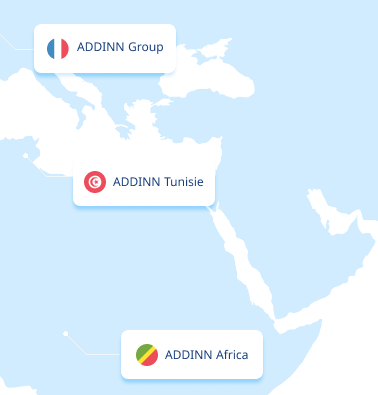
\includegraphics[width=\linewidth]{chapitres/ch1/img/map.PNG}
                \caption{\centering Présence internationale d'ADDINN\cite{apropos}}
                \label{fig:presence_addinn}
            \end{figure}
        \end{minipage}
        \begin{table}[H]
            \centering
            \caption{Étapes Clés d'Évolution d’ADDINN\cite{apropos}}
            \renewcommand{\arraystretch}{1.5}
            \begin{tabular}{|l|p{15cm}|}
                \hline
                \textbf{Année} & \textbf{Événement} \\
                \hline
                \textbf{2015} & Fondation d’ADDINN Group en France, spécialisé dans le conseil en IT. \\
                \hline
                \textbf{2018} & Création de la Digital \& Software Factory, dédiée au développement de solutions numériques sur mesure. \\
                \hline
                \textbf{2022} & Filialisation du groupe avec la création d’ADS Foundry, BeeWay Advisory et Qualifactory, ouvrant une nouvelle phase de développement et de croissance.  \\
                \hline
            \end{tabular}
            \label{tab:etapes_addinn}
        \end{table}
    \vspace{-0.6cm}
\subsection{Secteurs d'expertise et partenaires stratégiques} 
    L'expertise d'ADDINN couvre divers secteurs tels que l'assurance, la banque, le secteur public et le transport, offrant des solutions sur mesure. De plus, l'entreprise collabore avec plusieurs partenaires pour renforcer son offre et sa compétitivité, comme l'illustre la figure \ref{fig:Partenaires}.
    \vspace{-0.3cm}
    \begin{figure}[H]
        \centering
        \renewcommand{\thesubfigure}{}
        \subfloat{
\includegraphics[width=0.16\textwidth]{chapitres/ch1/img/partenaires/a1.png}}
        \subfloat{
\includegraphics[width=0.155\textwidth]{chapitres/ch1/img/partenaires/a2.png}} 
        \subfloat{
\includegraphics[width=0.13\textwidth]{chapitres/ch1/img/partenaires/a9.png}}
        \subfloat{
\includegraphics[width=0.14\textwidth]{chapitres/ch1/img/partenaires/a10.png}}
        \subfloat{
\includegraphics[width=0.15\textwidth]{chapitres/ch1/img/partenaires/a5.png}}
        \subfloat{
\includegraphics[width=0.15\textwidth]{chapitres/ch1/img/partenaires/a11.png}}
        \subfloat{
\includegraphics[width=0.14\textwidth]{chapitres/ch1/img/partenaires/a3.jpg}} \\
        
        \subfloat{
\includegraphics[width=0.17\textwidth]{chapitres/ch1/img/partenaires/a4.png}}
        \subfloat{
\includegraphics[width=0.19\textwidth]{chapitres/ch1/img/partenaires/a12.png}}
        \subfloat{
\includegraphics[width=0.19\textwidth]{chapitres/ch1/img/partenaires/a7.png}}
        \subfloat{
\includegraphics[width=0.14\textwidth]{chapitres/ch1/img/partenaires/a19.png}} 
        \subfloat{
\includegraphics[width=0.15\textwidth]{chapitres/ch1/img/partenaires/a6.png}}
        \subfloat{
\includegraphics[width=0.19\textwidth]{chapitres/ch1/img/partenaires/a17.png}}\\
        
        \subfloat{
\includegraphics[width=0.17\textwidth]{chapitres/ch1/img/partenaires/a13.png}}
        \subfloat{
\includegraphics[width=0.22\textwidth]{chapitres/ch1/img/partenaires/a8.png}}
        \subfloat{
\includegraphics[width=0.17\textwidth]{chapitres/ch1/img/partenaires/a14.png}}
        \subfloat{
\includegraphics[width=0.17\textwidth]{chapitres/ch1/img/partenaires/a15.png}} 
        \subfloat{
\includegraphics[width=0.17\textwidth]{chapitres/ch1/img/partenaires/a16.png}}
        \subfloat{
\includegraphics[width=0.135\textwidth]{chapitres/ch1/img/partenaires/a18.png}}\\
        \caption{Partenaires stratégiques d'ADDINN \cite{Addinn}}
        \label{fig:Partenaires}
    \end{figure}    
    \vspace{-0.7cm}
    \section{Étude de l’existant}
        \vspace{-0.1cm}
L’étude de l’existant permet d’identifier les points forts et les limites de l’application actuelle, ainsi que d’analyser les solutions similaires, afin d’orienter le développement d’une nouvelle version mieux adaptée aux besoins des utilisateurs.
\subsection{État actuel de l'application existante}
    L’application \textbf{PENTRA} (Figure~\ref{fig:PENTRA-V1-1}) constitue une première version d’un outil automatisé de tests de pénétration, développée dans le cadre d’un projet de fin d’études réalisé l’année précédente au sein de la société \textbf{ADDINN}. Elle a permis de poser les bases sur lesquelles s’appuient les évolutions futures envisagées dans le cadre de notre projet actuel.    
    \begin{figure}[H]
        \centering
        
\includegraphics[width=\linewidth]{Annexe/PENTRA-V1/1.PNG}
        \caption{\centering Interface de la page d'accueil PENTRA}
        \label{fig:PENTRA-V1-1}
    \end{figure}
    \vspace{-0.3cm}
    \subsubsection{Analyse de la solution existante}  
        Il s’agit d’une solution de détection des vulnérabilités web, reposant principalement sur l’intégration de deux outils de scan réputés, largement reconnus dans le domaine de la cybersécurité :
        \begin{itemize}[label=$-$]
            \item  \textbf{OWASP ZAP (Zed Attack Proxy)}: Un scanner open source développé par l’OWASP pour identifier les failles de sécurité dans les applications web, telles que les injections SQL, les failles XSS, les problèmes d’authentification ou les erreurs de configuration. Il propose des analyses actives et passives, une interface graphique riche, ainsi qu’une API permettant son automatisation.\cite{zap}.
            \item \textbf{Wapiti}: un outil open source d’analyse de vulnérabilités web basé sur des tests d’injection, qui scanne les sites web à la recherche de failles comme les injections de commande, les XSS ou encore les inclusions de fichiers. Il se distingue par sa légèreté et son approche modulaire.\cite{wapiti}.  
        \end{itemize}
         Cette solution est développée avec Angular (version 15), FastAPI et PostgreSQL, et intègre les fonctionnalités clés suivantes:
        \begin{itemize}[label=$\bullet$, left=0.2cm]
             \item \textbf{Gestion de l’authentification\footnote{Voir annexe A: Figures \ref{fig:PENTRA-V1-2} et \ref{fig:PENTRA-V1-3}}:} Interfaces d'inscription et de connexion permettant aux utilisateurs de créer un compte et d'accéder à la plateforme via leurs identifiants.
            \item \textbf{Lancement du scan\footnote{Voir Annexe A: Figure \ref{fig:PENTRA-V1-4}}:} L’utilisateur saisit l’URL du site web à analyser dans le champ prévu. Les 2 outils de scan sont lancés et fonctionnent en mode multithread, ce qui permet de traiter plusieurs requêtes simultanément et d’accélérer le processus.
            \item \textbf{Tableau des résultats du scan par outil\footnote{Voir annexe A: Figures \ref{fig:PENTRA-V1-7}, \ref{fig:PENTRA-V1-8} et \ref{fig:PENTRA-V1-9}}:} Deux interfaces présentant les résultats des scans sous forme de tableaux, avec la possibilité de télécharger les rapports détaillés au format PDF, offrant ainsi une vue d'ensemble des vulnérabilités détectées.
            \item \textbf{Paramétrage de l’envoi des rapports\footnote{Voir annexe A: Figure \ref{fig:PENTRA-V1-10}}:} permet de configurer l’envoi automatique des rapports vers Slack, Jira et par e-mail.
            \item \textbf{Tableaux de bord\footnote{Voir annexe A: Figures \ref{fig:PENTRA-V1-5} et \ref{fig:PENTRA-V1-6}}:} Chaque outil dispose de sa propre interface, affichant les résultats des scans, leur progression, ainsi que des charts graphiques statiques.
            \item \textbf{Gestion des profils\footnote{Voir annexe A: Figures \ref{fig:PENTRA-V1-11}}:} Permet aux utilisateurs de modifier leurs informations personnelles.
            \item \textbf{Gestion des utilisateurs et des rapports de scan\footnote{Voir annexe A: Figures \ref{fig:PENTRA-V1-12} et \ref{fig:PENTRA-V1-13}}:} L’administrateur peut gérer les comptes utilisateurs ainsi que consulter, organiser et superviser les rapports des scans.
        \end{itemize}
    \subsubsection{Limites et critiques de la solution existante}
    L’application présente plusieurs lacunes affectant son ergonomie, ses performances et ses fonctionnalités. Ces limitations doivent être corrigées pour améliorer son efficacité globale.
        \begin{itemize}[label=\textcolor{red}{\ding{56}}]
            \item \textbf{Problèmes liés aux processus de scan et à la génération des rapports:}\\
            Les processus actuels de scan et de génération de rapports présentent plusieurs lacunes qui nuisent à la clarté des résultats, à l’ergonomie des interfaces et à l’efficacité globale de l’analyse. Parmi les problèmes relevés, on peut citer :
                \begin{itemize}[label=$\bullet$, left=-0.05cm]
                    \item \textbf{Surcharge d’informations:} Les tableaux des résultats des scans et les rapports générés sont excessivement longs et contiennent souvent des informations inutiles.
                   \item \textbf{Affichage de résultats non optimisés et non pertinents :} La présence de vulnérabilités avec un compteur égal à zéro, ainsi que de champs excessivement détaillés ou peu utiles, nuit à la lisibilité et complique l’analyse des résultats. Ce manque d’optimisation rend l’interprétation des rapports plus difficile et chronophage.
                    \item \textbf{Incohérence dans la structure des tableaux:} Les colonnes varient entre les outils, compliquant la comparaison des résultats. De plus, l'absence de filtres ou d'options de recherche pour trier les données rend leur exploitation moins efficace.
                    \item \textbf{Problèmes de progression des scans:} Les outils affichent la progression différemment: ZAP utilise une barre de progression, tandis que Wapiti le fait sous forme textuelle indiquant les modèles scannés, ce qui crée une incohérence.
                    \item \textbf{Navigation peu intuitive entre les interfaces des résultats:} La navigation entre les interfaces est confuse, ce qui complique la lecture et l’interprétation des résultats, notamment sur les tableaux de bord de Wapiti et ZAP ainsi que sur les deux tableaux de résultats, rendant l’analyse des vulnérabilités plus difficile.
                    \item \textbf{Mauvaise gestion des scans simultanés:} Le système actuel ne gère pas correctement les lancements parallèles ou successifs de plusieurs scans par le même utilisateur ou par plusieurs utilisateurs. Cela provoque une surcharge du backend, des conflits d’accès aux ressources, voire un blocage partiel de l’application. De plus, certains outils sont déclenchés plusieurs fois en parallèle, entraînant des erreurs d’exécution et empêchant la génération des rapports.
                    \item \textbf{Diffusion des rapports limitée :} Les e-mails contenant les rapports\footnote{Voir annexe A: Figure \ref{fig:PENTRA-V1-email}} sont trop basiques manquent de clarté et de modernité. Par ailleurs, l’envoi des rapports via Slack et Jira ne fonctionne pas de manière fiable. L’absence d’options de téléchargement aux formats HTML, JSON et CSV limite l’exportation et rend difficile l’analyse approfondie des résultats ou leur intégration avec d’autres outils.
                \end{itemize}
            \item \textbf{Couverture incomplète des types d’audits:} Le système actuel se concentre principalement sur les audits de sécurité mais ne prend pas en charge l’ensemble des autres formes d’analyse essentielles. Il n’intègre ni les tests fonctionnels ni les audits SEO. Cette limitation réduit la portée globale des évaluations et empêche une vision complète de l’état et de la qualité du site web.
            \item \textbf{Limites de la structure de la base de données :}La base repose sur deux tables (\texttt{utilisateur} et \texttt{rapport})\footnote{Voir Annexe A : Figure \ref{fig:PENTRA-db-initial}}, dans lesquelles les rapports sont stockés au format binaire sans structuration interne. Cette approche entraîne un manque de granularité empêchant l’interrogation directe d’éléments clés comme les vulnérabilités. Elle limite les capacités de recherche, de filtrage et d’agrégation des données via des requêtes SQL standards. À mesure que le volume de rapports augmente, cette structure nuit à la scalabilité et à la performance de la base en ralentissant l’accès aux données en augmentant la consommation de ressources et en rendant l’exploitation des données particulièrement difficile.
            \item \textbf{Problèmes des tableaux de bord statiques:} Les graphiques ne sont pas fonctionnels et restent statiques, empêchant une visualisation dynamique et claire des vulnérabilités. 
            \item \textbf{Navigation confuse :} La coexistence d’une barre supérieure et d’une barre latérale de navigation mal structurées crée une expérience utilisateur désorientante, avec des liens incohérents, inutiles ou bloqués.
            \item \textbf{Ancienne version d’Angular:}  L’application utilise actuellement Angular version 15, qui est dépassée et n’est plus utilisée par la société. Une migration vers une version plus récente est nécessaire.
            \item \textbf{Affichage non responsive:} Les interfaces ne sont pas totalement responsives, limitant une utilisation fluide sur différents types d’écrans (tablettes, mobiles, etc.).
            \item \textbf{Accès non sécurisé aux interfaces sans authentification:} Bien que l’accès au backend soit protégé par authentification (erreur 403 en cas d’accès non autorisé), l’utilisateur peut accéder librement au frontend (dashboard, historique des scans, page de scan) sans authentification, ce qui crée une incohérence dans la gestion des droits d’accès.
            \item \textbf{Absence de gestion des mots de passe:} Il manque les pages dédiées à la réinitialisation ou à la récupération du mot de passe oublié, ce qui empêche les utilisateurs de récupérer l’accès à leur compte en cas d’oubli.
         \end{itemize}
    Des améliorations importantes sont indispensables afin d’optimiser l’ergonomie, les fonctionnalités et la sécurité de l’application, tout en offrant une meilleure expérience utilisateur. 
        \begin{justify}
    \subsection{Analyse et critique des applications similaires}
    L’analyse des applications concurrentes permet d’identifier les axes d’amélioration, afin d’optimiser notre solution et de concevoir une expérience utilisateur répondant aux attentes du marché.
    \subsubsection{Outils d’automatisation des tests de pénétration\cite{etdeExistant}}
        Un scanner de vulnérabilités analyse un site web afin de détecter les risques liés au code source et aux liens en identifiant des menaces telles que les malwares, les injections SQL, les failles XSS. Le choix d’un outil dépend de plusieurs critères: la complexité du site, la couverture des vulnérabilités, la qualité des rapports générés et la capacité à effectuer des analyses régulières\cite{etdeExistant}.

        Nous avons sélectionné les outils suivants comme solutions similaires à notre application dans la partie dédiée aux tests de pénétration, afin d’en analyser les fonctionnalités et les limites.
        \begin{enumerate}[label=\alph*)]
            \item \textbf{HostedScan\cite{etdeExistant}:} est un service en ligne basé sur des scanners 100\% open-source, il automatise la détection des vulnérabilités sur les réseaux, serveurs et applications web. Il centralise la gestion des failles, facilite la priorisation des tâches, la génération de rapports, et renforce la sécurité de leurs clients. Ce service inclut plusieurs types de scanners:  
            \begin{itemize}[label=$\bullet$]
                    \item \textbf{Des vulnérabilités réseau}: identifie les \acs{CVE} et les logiciels obsolètes.  
                    \item \textbf{Des applications web}: détecte les injections SQL, les bibliothèques JavaScript vulnérables, les scripts intersites (\acs{XSS}) et autres menaces.  
                    \item \textbf{Des ports TCP/UDP}: repère les erreurs de configuration des pare-feu et du réseau.  
                    \item \textbf{TLS/SSL}: valide les certificats et recherche les vulnérabilités Heartbleed et Robot.  
                \end{itemize}
                
            La Figure~\ref{fig:Hostedscan} présente l’interface du tableau de bord de l’application HostedScan, illustrant les résultats des analyses ainsi que les principales fonctionnalités proposées.
                \begin{figure}[H]
                    \centering
                   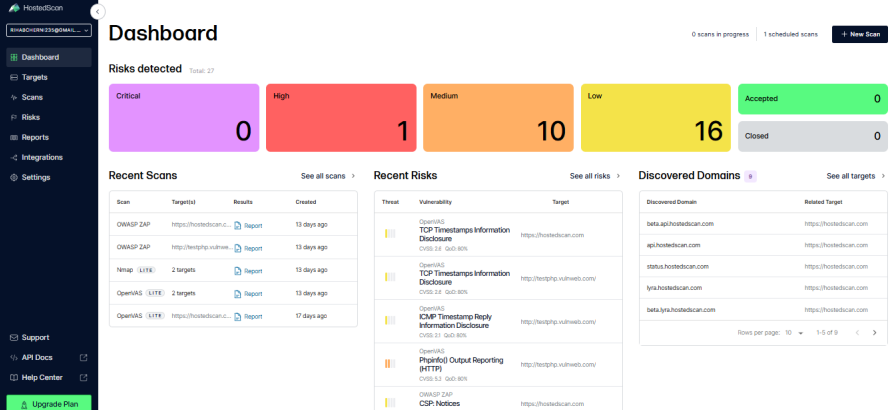
\includegraphics[width=\textwidth]{chapitres/ch1/img/existant/hostedscan.PNG}
                    \caption{Interface du l’application Hostedscan\cite{hostedscanimg}}
                    \label{fig:Hostedscan}
                \end{figure}
            \vspace{-0.1cm}
            \item \textbf{Invicti\cite{invicti} :} est un outil de sécurité web avancé permettant de protéger les applications, services web et API contre une large gamme de vulnérabilités, telles que les injections SQL, les failles \acs{XSS} et les erreurs de configuration SSL/TLS. Il réalise également des tests de configuration des serveurs web et se distingue par son moteur d’analyse basé sur la preuve, qui confirme automatiquement l’exploitabilité des failles détectées, réduisant ainsi les faux positifs. Son moteur d’exploration intelligent est compatible avec les technologies dynamiques modernes (JavaScript, Ajax, React, Angular), ce qui le rend efficace pour l’analyse des applications complexes.\\Invicti s’intègre facilement aux pipelines DevOps et CI/CD, favorisant une automatisation continue de la sécurité. Il propose en outre des tableaux de bord interactifs, des rapports personnalisables et des fonctionnalités de gestion des vulnérabilités, facilitant la collaboration entre les développeurs et les équipes de sécurité.
            
            La Figure~\ref{fig:Invicti} montre l’interface de l’outil Invicti, mettant en évidence les résultats d’analyse de sécurité web ainsi que les fonctionnalités de gestion des vulnérabilités.
            \begin{figure}[H]
                \centering
               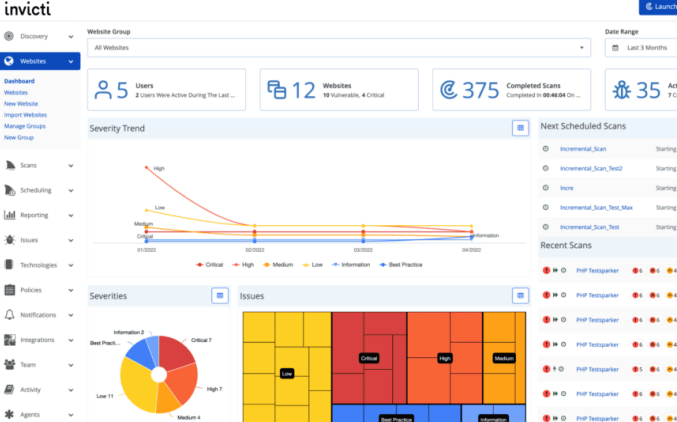
\includegraphics[width=\textwidth]{chapitres/ch1/img/existant/invicti.png}
                \caption{Interface du l’application Invicti\cite{invicti}}
                \label{fig:Invicti}
            \end{figure}
            \vspace*{-0.4cm}
        \end{enumerate}
    \subsubsection{Outils d’automatisation des tests fonctionnels:}
        L’automatisation des tests fonctionnels est essentiel pour assurer la qualité et la fiabilité des applications. Plusieurs outils sont disponibles qui offrent des fonctionnalités variées comme:
        \begin{enumerate}[label=\alph*)]
           \item  \textbf{Cypress}\cite{Cypress} est un outil d'automatisation de tests fonctionnels pour les applications web, apprécié pour sa rapidité, sa fiabilité et sa simplicité d'utilisation. Il permet d’automatiser des tests de composants, d’API et d’accessibilité, tout en assurant la compatibilité multi-navigateurs. Grâce à son interface de débogage en temps réel, son exécution locale rapide et sa facilité d’intégration, il constitue une solution complète pour les tests web.

           La Figure~\ref{fig:Cypress} illustre l’environnement de test automatisé proposé par Cypress, affichant les scénarios exécutés, les résultats des tests, et les options de débogage.
                \begin{figure}[H]
                \centering
               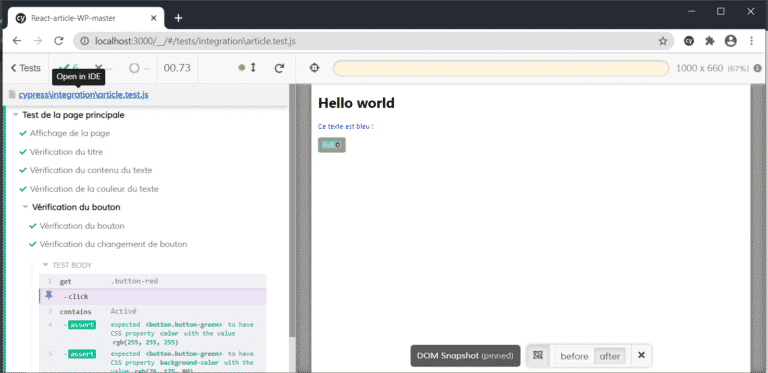
\includegraphics[width=\textwidth]{chapitres/ch1/img/existant/cpress.PNG}
               \caption{Interface de démonstration de Cypress exécutant une suite de tests \cite{imgCypress}}
                \label{fig:Cypress}
            \end{figure}
                \vspace{-0.4cm}
            \item  \textbf{Katalon Studio\cite{Katalon}:} est un outil d'automatisation des tests pour les applications web et mobiles, basé sur Selenium. Il offre une interface conviviale permettant de créer et d’exécuter des tests sans compétences techniques avancées. Son intégration avec des outils comme Jira et Slack, ainsi que son support des tests continus et du suivi instantané des résultats, en fait une solution efficace pour assurer la qualité tout au long du développement.

            La Figure~\ref{fig:Katalon-Studio} présente l’interface de Katalon Studio, illustrant l’organisation des cas de test ainsi que le suivi de leur exécution.
            \begin{figure}[H]
                \centering
                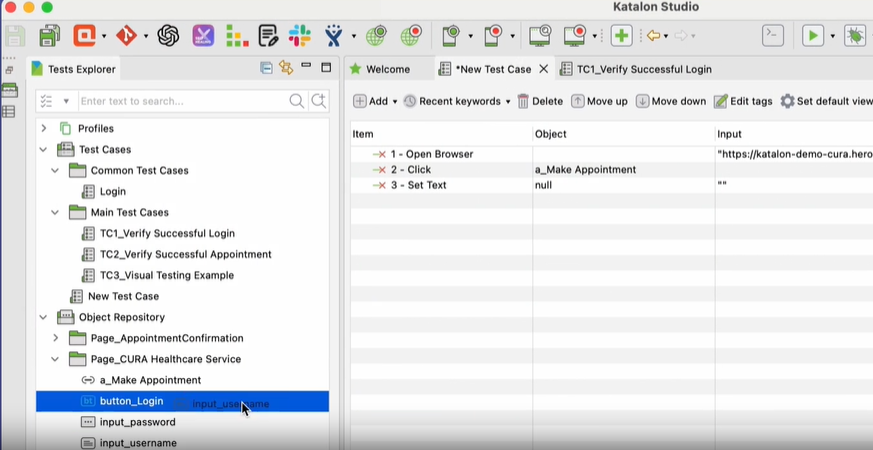
\includegraphics[width=\textwidth]{chapitres/ch1/img/existant/katal.PNG}
                \caption{Interface du l’application Katalon Studio\cite{Katalon}}
                \label{fig:Katalon-Studio}
            \end{figure}
            \vspace{-0.3cm}
    \end{enumerate}
    
    \subsubsection{Outils d’automatisation des tests SEO}
        Le \textbf{SEO (Search Engine Optimization)} est indispensable pour renforcer la visibilité d’un site sur les moteurs de recherche.Il permet d’identifier les erreurs, d’optimiser les performances et de vérifier le respect des bonnes pratiques. Plusieurs outils automatisent ces audits en analysant les mots-clés, le contenu, les aspects techniques, le positionnement, et en générant des recommandations et des rapports. Voici une analyse des plus pertinents.  
        \begin{enumerate}[label=\alph*)]
            \item \textbf{Semrush\cite{seoTools}:} est un outil SEO les plus populaires et complets du marché. Il propose une large gamme de fonctionnalités: l’analyse de mots-clés, l’audit technique, la veille concurrentielle, le suivi de positionnement, la gestion des backlinks, l’analyse du temps moyen passé sur le site ainsi que l’identification des pages les plus performantes. Son outil de suivi de positionnement fournit des analyses précises et évolutives, permettant aux professionnels du marketing digital de surveiller efficacement la performance de leurs mots-clés sur les moteurs de recherche. Il permet également de réaliser des audits SEO détaillés et de générer des rapports visuels pour le suivi des performances dans le temps.

            La Figure~\ref{fig:Semrush} illustre le tableau de bord de SEMrush, mettant en évidence les résultats de l’audit SEO ainsi que les performances globales du site web.
            \begin{figure}[H]
                \centering
                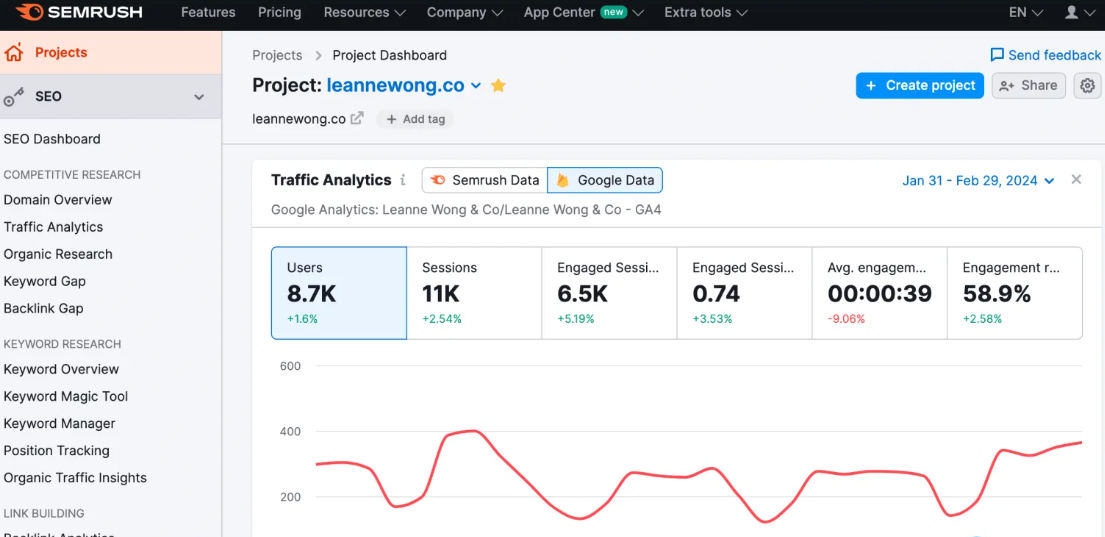
\includegraphics[width=\textwidth]{chapitres/ch1/img/existant/semrush.PNG}
                \caption{Interface de l’outil Semrush\cite{seoTools}}
                \label{fig:Semrush}
            \end{figure}
        \vspace{-0.3cm}
        \item \textbf{Ahrefs\cite{seoTools}} est une plateforme SEO reconnue pour la puissance de sa base de données de backlinks et ses capacités avancées d’analyse concurrentielle. Elle permet d’ajuster efficacement sa stratégie de contenu en observant les performances des concurrents sur les moteurs de recherche. L’outil offre des fonctionnalités telles que le suivi du positionnement des mots-clés, l’identification des pages les plus génératrices de trafic, l’analyse des liens entrants et l’accès à l’historique du positionnement via des visualisations graphiques.

        La Figure~\ref{fig:AhrefsAudit} présente l’interface d’Ahrefs, mettant en évidence le suivi du positionnement ainsi que les principaux indicateurs de performance SEO.
            \begin{figure}[H]
                \centering
                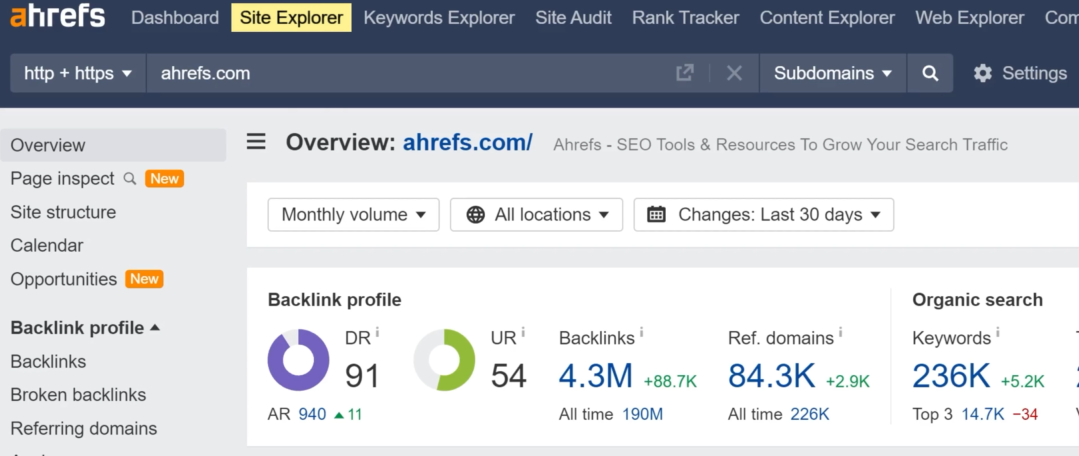
\includegraphics[width=\textwidth]{chapitres/ch1/img/existant/ahrefs.PNG}
                \caption{Interface de l’outil Ahrefs Site Audit\cite{seoTools}}
                \label{fig:AhrefsAudit}
            \end{figure}
            \vspace{-0.3cm}
        \end{enumerate}    
    \subsubsection{Critique de l’existant:}
        Le tableau ~\ref{tab: comparaison} présente une  comparaison détaillée des principaux outils analysés précédemment.
        \begin{spacing}{1.5}
            \begin{longtable}{|p{2.7cm}|p{6.6cm}|p{6.6cm}|}
                \caption{\centering Tableau comparatif des outils d’automatisation}
                \label{tab: comparaison}\\ \hline
                         \multicolumn{3}{|c|}{\textbf{Outils d’automatisation des tests de pénétration \cite{etdeExistant}}} \\
                        \hline
                        \textbf{Application} & \textbf{HostedScan} & \textbf{Invicti}\\
                        \hline
                            \textbf{Score}\footnote{Le score Geekflare est attribué par une équipe éditoriale selon plusieurs critères techniques et fonctionnels (source : \href{https://geekflare.com/fr/cybersecurity/best-website-security-scanner/}{Geekflare}).}& 
                                4.2/5 &
                                4.5/5
                                \\  \hline
                             \begin{minipage}[t]{2.8cm}
                                \textbf{Profondeur d’analyse}
                            \end{minipage}& 
                            \begin{minipage}[t]{6.6cm}
                                 \justifying Réseaux, serveurs, applications web
                            \end{minipage}
                                &
                             \begin{minipage}[t]{6.6cm}
                                 \justifying API, sites, applications, services et serveurs web.
                                 \vspace{0.2cm}
                            \end{minipage}
                            \\ 
                        \hline
                             \begin{minipage}[t]{2.9cm}
                                 \textbf{Fonctions principales}
                            \end{minipage}& 
                            \begin{minipage}[t]{6.6cm}
                                 \justifying Scanners open-source et gestion centralisée des vulnérabilités.
                            \end{minipage}
                                &
                            \begin{minipage}[t]{6.6cm}
                                 \justifying Analyse basée sur la preuve et exploitation automatique des vulnérabilités.
                                \vspace{0.2cm}
                            \end{minipage}\\ 
                        \hline
                            \textbf{Avantages} & 
                                \begin{minipage}[t]{6.6cm}
                                     \justifying
                                    \begin{itemize}[left=-0.1cm, label=\textcolor{green}{$\checkmark$}]
                                        \item Détection et notification en temps réel des menaces  
                                        \item Analyse approfondie.
                                        \item Rapports personnalisables.
                                        \item Offre un plan gratuit.  
                                    \end{itemize}
                                    \vspace{0.1cm}
                                \end{minipage}
                                &
                                \begin{minipage}[t]{6.6cm}
                                     \justifying 
                                    \begin{itemize}[left=-0.1cm, label=\textcolor{green}{$\checkmark$}]
                                        \item Excellent support client.
                                        \item Fournit des rapports et des analyses détaillés.
                                        \item Faible nombre de faux positifs.
                                    \end{itemize}
                                \end{minipage}\\ 
                            \hline
                            \textbf{Inconvénients} & 
                                \begin{minipage}[t]{6.6cm}
                                     \justifying
                                    \begin{itemize}[left=-0.1cm, label=\textcolor{red}{\ding{56}}]
                                        \item Interface utilisateur peu ergonomique  
                                         \item Limité aux scanners open-source 
                                    \end{itemize}
                                    \vspace{0.1cm}
                                \end{minipage} &
                                \begin{minipage}[t]{6.6cm}
                                     \justifying
                                    \begin{itemize}[left=-0.1cm, label=\textcolor{red}{\ding{56}}]
                                        \item Absence de tarification initiale.
                                        \item Les analyses prennent parfois beaucoup de temps
                                    \end{itemize}
                                \end{minipage}\\
                            \hline
                            \textbf{Tarification} & 
                               \begin{minipage}[t]{6.6cm}
                                     \justifying
                                    \begin{itemize}[left=-0.1cm, label=$\bullet$]
                                        \item \textbf{Gratuit}: 3 analyses par mois  
                                        \item \textbf{Basique}: 39\$ mois  
                                        \item \textbf{Premium}:109\$ mois
                                    \end{itemize}
                                    \vspace{0.1cm}
                                \end{minipage}
                                &
                                \begin{minipage}[t]{6.6cm}
                                     \justifying  Offre des prix personnalisés en fonction de vos besoins spécifiques.
                                \end{minipage}\\ 
                           \hline
    
                          \multicolumn{3}{|c|}{\textbf{Outils d’automatisation des tests fonctionnels\cite{,compTestFon2}}} \\
                        \hline
                        
                        \textbf{Application} & \textbf{Cypress} & \textbf{Katalon Studio} \\
                        \hline
                            \textbf{Score}\footnote{Le score Capterra reflète la moyenne des avis des utilisateurs sur différents critères (ergonomie, fonctionnalités, support, rapport qualité/prix)(source: \href{https://clickup.com/fr-FR/blog/228197/les-outils-de-test-d'automatisation}{ClickUp}).}
                            & 4.7/5& 4.4/5 \\ 
                        \hline
                            \begin{minipage}[t]{2.8cm}     
                                \textbf{Profondeur d’analyse}
                            \end{minipage}& 
                            \begin{minipage}[t]{6.6cm}
                                 \justifying Tests: de bout en bout, de composants, d’API, d'accessibilité.
                                 \vspace{0.1cm}
                            \end{minipage}
                                & 
                            \begin{minipage}[t]{6.6cm}
                                 \justifying Tests: UI, d'API, de charge, de performance des applications web.
                                \vspace{0.1cm}
                            \end{minipage} 
                            \\ 
                        \hline
                            \textbf{Avantages} & 
                                \begin{minipage}[t]{6.8cm}
                                    \begin{itemize}[left=-0.1cm, label=\textcolor{green}{$\checkmark$}]
                                        \item Exécution rapide, compatible multi-navigateurs.
                                        \item Facilité de configuration.
                                        \item Débogage puissant avec l'interface graphique.
                                        \item Tests fiables et résultats cohérents.
                                    \end{itemize}
                                    \vspace{0.1cm}
                                \end{minipage}
                                &
                                \begin{minipage}[t]{6.6cm}
                                     \justifying
                                    \begin{itemize}[left=-0.12cm, label=\textcolor{green}{$\checkmark$}]
                                        \item Facilité d'utilisation.
                                        \item Documentation complète et support client efficace.
                                        \item Intégration facile avec les pipelines CI/CD.
                                        \item Compatibilité multi-navigateurs et tests multiplateformes.
                                    \end{itemize}
                                    \vspace{0.1cm}
                                \end{minipage}
                                \\ 
                        \hline
                            \textbf{Inconvénients} & 
                                \begin{minipage}[t]{6.6cm}
                                     \justifying
                                    \begin{itemize}[left=-0.1cm, label=\textcolor{red}{\ding{56}}]
                                        \item Certains utilisateurs ont constaté des bugs.
                                        \item Manque d'assistance intégrée pour les tests d'applications mobiles.
                                    \end{itemize}
                                \end{minipage} &
                                \begin{minipage}[t]{6.6cm}
                                     
                                    \justifying
                                    \begin{itemize}[left=-0.1cm, label=\textcolor{red}{\ding{56}}]
                                        \item Décalage lors de l'utilisation sur certains ordinateurs portables.
                                        \item Des fonctionnalités manquantes comme l'exécution parallèle.
                                    \end{itemize}
                                    \vspace{0.1cm}
                                \end{minipage}  \\
                        \hline
                            \textbf{Tarification} & 
                               \begin{minipage}[t]{6.6cm}
                                    \begin{itemize}[left=-0.1cm, label=$\bullet$]
                                        \item \textbf{Gratuit}: Plan communautaire limité
                                        \item \textbf{Équipes}: 75\$/mois.
                                        \item \textbf{Business}: 300\$/mois
                                        \item \textbf{Entreprise}: Prix personnalisé.
                                    \end{itemize}
                                    \vspace{0.1cm}
                                \end{minipage}&
                                 \begin{minipage}[t]{6.6cm}
                                     \justifying
                                    \begin{itemize}[left=-0.15cm]
                                        \item[$\bullet$] \textbf{Gratuit}: 0\$ (Plan de base avec certaines limitations).
                                        \item[$\bullet$] \textbf{Premium}: 218\$/utilisateur/mois  
                                        \item[$\bullet$] \textbf{Entreprise}: Prix personnalisé.
                                    \end{itemize}
                                    \vspace{0.1cm}
                                \end{minipage} 
                                \\ 
                       \hline
                       \multicolumn{3}{|c|}{\textbf{Outils d’audit SEO automatisé\cite{seoTools}}} \\
                        \hline
                        \textbf{Application} & \textbf{Semrush}& \textbf{Ahrefs Site Audit} \\
                        \hline
                            \textbf{Score}\footnote{Le score Capterra correspond à la moyenne des avis utilisateurs, évaluant des critères tels que l’ergonomie, les fonctionnalités, le support et le rapport qualité/prix (sources : \href{https://www.capterra.com/p/176340/Ahrefs/}{Ahrefs} et \href{https://www.capterra.com/p/151962/SEMrush/}{SEMrush}).}
                            & 4.6/5& 4.7/5 \\ 
                        \hline 
                        \textbf{Interface utilisateur} & 
                        Simple, intuitive et rapide à utiliser & 
                        Tableaux de bord graphiques et interactifs \\
                        \hline   
                        \textbf{Fonctions principales} & 
                        Audit HTML, SEO on-page, détection de liens cassés, analyse de la vitesse, compatibilité mobile, avec export des 1résultats en PDF & Visualisation graphique, suivi des erreurs, historique des audits, recommandations, avec export des résultats sous forme de graphiques et de rapports web \\
                        \hline
                        \textbf{Avantages} & 
                       \begin{minipage}[t]{6.6cm}
                            \begin{itemize}[left=-0.15cm, label=\textcolor{green}{$\checkmark$}]
                               \item Recherche et suivi des mots-clés.
                               \item Analyse concurrentielle.
                               \item Suivi du positionnement en temps réel.
                               \item Audit technique SEO complet.
                               \item Optimisation des backlinks.
                               \item Interface personnalisable.
                             \end{itemize}
                        \end{minipage}& 
                         \begin{minipage}[t]{6.6cm}
                            \begin{itemize}[left=-0.15cm, label=\textcolor{green}{$\checkmark$}]
                                \item Base de données de backlinks ultra-complète.
                                \item Analyse approfondie des sites concurrents pour identifier leurs stratégies SEO.
                                \item Suivi précis des performances et suggestions de contenu pertinentes.
                            \end{itemize} 
                            \vspace{0.05cm}
                        \end{minipage}\\
                        \hline 
                        \textbf{Inconvénients} & 
                         \begin{minipage}[t]{6.6cm}
                            \begin{itemize}[left=-0.15cm, label=\textcolor{red}{\ding{56}}]
                                \item Tarification élevée pour les petites entreprises.
                                \item Une interface complexe pour les débutants.
                            \end{itemize}
                            \vspace{0.1cm}
                        \end{minipage}& 
                         \begin{minipage}[t]{6.6cm}
                            \begin{itemize}[left=-0.15cm, label=\textcolor{red}{\ding{56}}]
                                \item Moins complet que Semrush pour l’optimisation on-site.
                                \item Peu d’options pour générer des rapports personnalisés.
                            \end{itemize}
                            \vspace{0.1cm}
                        \end{minipage}\\
                        \hline
                    \end{longtable}
        \end{spacing}
        \vspace{-0.4cm}
        Chaque outil présente des atouts spécifiques selon le type de tests à automatiser, qu’il s’agisse de sécurité, de fonctionnalité ou d’audit SEO. Le choix de l’outil dépendra des besoins techniques, du budget disponible et du niveau d’intégration souhaité dans le processus de développement.
\end{justify}
    \section{Problématique}
        Les tests fonctionnels, les tests de sécurité ainsi que les tests SEO représentent trois aspects essentiels pour garantir la fiabilité, la performance et la visibilité des applications. Toutefois, leur mise en œuvre reste principalement manuelle, ce qui la rend chronophage et sujette à des erreurs humaines. \\
La question qui se pose est de concevoir une solution capable d’automatiser ces types de tests tout en assurant une couverture complète et une analyse fiable?



    \section{Solution proposée}
        Afin de surmonter les nombreuses limites identifiées dans l’application existante, la solution proposée vise à développer une plateforme complète pour l’automatisation des tests de sécurité, des audits SEO, et des tests fonctionnels avec une analyse fiable et complète des résultats. Elle vise à renforcer la visibilité des applications tout en garantissant leur bon fonctionnement. Cette nouvelle solution repose sur une approche intégrée et évolutive avec les objectifs suivants:
\begin{itemize}[label=$\bullet$,left=0.09cm]
    \item \textbf{Intégration optimisée des outils de pénétration}: Utilisation de ZAP\cite{zap}, Wapiti\cite{wapiti}, Nuclei\cite{nuclei}, Nikto\cite{nikto}, SQLMap\cite{sqlmap}, XSStrike\cite{xsstrike} et autres, chacun spécialisé dans une famille de vulnérabilités, pour détecter les failles de sécurité et couvrir un périmètre d’analyse plus large et plus fiable.
    
    \item \textbf{Mécanisme de comparaison, de consolidation des résultats et de validation automatique des faux positifs}: regroupement des vulnérabilités similaires détectées par différents outils, avec une pondération selon leur niveau de risque, afin d’éliminer les doublons, de clarifier les rapports, d’améliorer leur précision, de filtrer les résultats pertinents, de réduire les erreurs de détection et d’optimiser le temps d’analyse.

    \item \textbf{Scan d’authentification automatisé}: Détection des formulaires de connexion après identification des champs login/password, cookies et tokens d’authentification pour permettre les scans dans les zones protégées en reproduisant des scénarios d’attaque.
    
    \item \textbf{Automatisation des tests fonctionnels}: en exécutant des scénarios de tests simulant le comportement utilisateur (remplissage de formulaires, clics, redirections), afin de vérifier que les fonctionnalités clés restent opérationnelles et conformes aux exigences des utilisateurs.
    
    \item \textbf{Automatisation des tests SEO}: pour analyser les techniques du référencement (temps de chargement, structure HTML, balises, liens cassés).
    
    \item \textbf{Système de reporting}: Génération de rapports synthétiques et clairs avec des filtres (par outil, par niveau de gravité, par catégorie), visualisation graphique interactive, export en PDF, HTML, JSON ou CSV, envoi par e-mail, Slack ou Jira.
    \item \textbf{Refonte de la base de données} : adoption d’une structure relationnelle optimisée avec des tables normalisées permettant un stockage détaillé des rapports, une gestion granulaire des vulnérabilités ainsi qu’une meilleure exploitation des données via des requêtes avancées.
    \item \textbf{Gestion intelligente des scans concurrents} : Mise en place d’un système de file d’attente et de verrouillage par utilisateur afin d’empêcher le lancement simultané ou successif non contrôlé de plusieurs scans. Une logique de planification permet d’exécuter les scans de manière ordonnée, tout en assurant un contrôle d’accès aux ressources partagées. Des vérifications en temps réel préviennent les doublons, les surcharges ou les blocages. Des statuts d’exécution offrent à l’utilisateur la possibilité de suivre l’avancement d’un scan ou de l’annuler si nécessaire.
    \item \textbf{Interface responsive et modernisée}: Refonte complète du frontend en Angular dernière version 18, accès contrôlé par authentification JWT\cite{jwt} et rôle utilisateur, et responsive design pour mobile et tablette.
    \item \textbf{Sécurisation complète des accès} : Mise en place d’un contrôle d’accès uniforme sur l’ensemble des routes, avec redirections automatiques, gestion des sessions et mécanisme de réinitialisation de mot de passe.
\end{itemize}
Cette solution permettra de corriger en profondeur les failles de l’application actuelle en rendant les processus de tests efficaces et compréhensibles. Elle contribuera aussi à fournir une plateforme unifiée adaptée aux besoins réels des développeurs, des testeurs et des responsables sécurité.

    \section{Choix méthodologique de travail}
    Les méthodes agiles proposent une approche flexible et itérative du développement, centrée sur la réduction des risques, l’adaptabilité et la satisfaction du client. Scrum est la méthode agile la plus couramment adoptée\cite{agile}.

Le choix méthodologique retenu pour notre application, défini dès le début du stage, résulte d’une réflexion collective. Il a été guidé par les besoins du projet et la stratégie de l’entreprise, notamment en matière d’approche, de langage de modélisation et de processus de développement.
\subsection{Fonctionnement général de Scrum\cite{Scrum}}
Scrum repose sur des itérations successives "sprints", comme l’illustre la figure \ref{fig:Scrum}, permettant une livraison progressive du produit et visant à apporter de la valeur au client en favorisant la transparence, la collaboration et l’amélioration continue.
\begin{figure}[H]
    \centering
    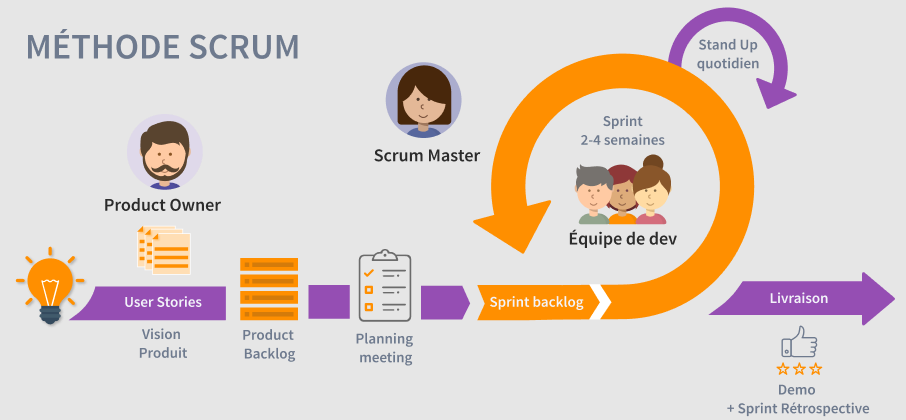
\includegraphics[width=\linewidth]{chapitres/ch1/img/scrum.PNG}
    \caption{Cadre méthodologique et mode de fonctionnement SCRUM \cite{ScrumImg}}
    \label{fig:Scrum}
\end{figure}
\vspace{-0.5cm}
L’équipe Scrum se compose de trois rôles clés:
\begin{itemize}[label=$\bullet$]
    \item \textbf{Product Owner:} Gère le backlog et définit les priorités selon les besoins client.
    \item \textbf{Scrum Master:} Garantit le respect de la méthodologie et facilite le travail de l’équipe.
    \item \textbf{Équipe de développement:} Chargée de la réalisation des fonctionnalités et de la livraison des incréments du produit.
\end{itemize}
\subsection{Événements Scrum\cite{Scrum}}
    Les événements Scrum assurent l’organisation et l’amélioration continue du processus:
    \begin{itemize}[label=$\bullet$]
        \item \textbf{Daily Scrum:} Réunion quotidienne de 15 minutes pour synchroniser le travail, partager les avancées et identifier les obstacles.
        \item \textbf{Sprint Review:} Présentation de l’incrément réalisé à la fin du sprint aux parties prenantes afin d'obtenir des retours et ajuster les priorités.
        \item \textbf{Sprint Retrospective:} Réunion d’équipe pour analyser ce qui a bien fonctionné, identifier les axes d’amélioration et optimiser les processus pour les futurs sprints.
    \end{itemize}
\subsection{Artefacts Scrum\cite{Scrum}}
    Les artefacts Scrum structurent le travail et assurent la transparence pour suivre l'évolution du projet et adapter les actions en conséquence. Parmi ces artefacts, on trouve :
    \begin{itemize}[label=$\bullet$]
        \item \textbf{Backlog produit :} liste évolutive des fonctionnalités, gérée par le \textbf{Product Owner}.
        \item \textbf{Backlog de sprint :} ensemble des tâches à réaliser durant un sprint.
        \item \textbf{Incrément de produit :} version fonctionnelle et enrichie du produit, livrée à la fin du sprint.
        \item \textbf{Burndown chart :} graphique illustrant l'avancement des tâches et la vélocité de l’équipe.
    \end{itemize}
\subsection{Avantages de Scrum\cite{Scrum}}
L’adoption de Scrum présente plusieurs avantages :
\begin{itemize}[label=$\bullet$]
    \item Meilleure qualité logicielle grâce aux tests fréquents et aux retours d’utilisateurs.
    \item Satisfaction client accrue, avec une réactivité face aux évolutions des besoins.
    \item Livraisons plus rapides, optimisant la mise en production des fonctionnalités prioritaires.
    \item Dynamique d’équipe améliorée, favorisant la motivation et l’autonomie des développeurs.
\end{itemize}  
    \section*{\texorpdfstring{Conclusion}{Conclusion}}
    \addcontentsline{toc}{chapter}{\textbf{Conclusion}}
    Ce chapitre a introduit le projet en présentant son contexte, les caractéristiques de l’organisme d’accueil, ainsi que les lacunes de l’outil existant et des solutions similaires, soulignant ainsi la nécessité d’adopter une nouvelle approche. Il a exposé la solution proposée et la méthodologie de travail. Le chapitre suivant portera sur l’analyse préliminaire de cette nouvelle solution.
\end{justify} \newpage
        \chapter{ Analyse et planification du projet}
\renewcommand{\thesection}{\arabic{section}}
\vspace{-0.3cm}
\begin{justify}
    \section*{\texorpdfstring{Introduction}{Introduction}}
    \addcontentsline{toc}{chapter}{\textbf{Introduction}}
    \begin{justify}
    Dans ce chapitre, nous allons présenter la première phase de la méthodologie Scrum qui est la phase de planification. Il comprend l’identification des acteurs, des besoins fonctionnels et non fonctionnels, la création du diagramme de cas d’utilisation, la présentation de l’équipe de travail, l’élaboration du backlog produit, ainsi que la planification des sprints. Nous y décrivons également l’environnement logiciel et matériel adopté, ainsi que l’architecture générale retenue.
\end{justify}


    
    \section{Spécification et analyse des besoins}
        \begin{justify}
            La capture des besoins permet au client d’exprimer ses attentes. Dans cette section, nous présentons les acteurs, les besoins fonctionnels et non fonctionnels que notre solution doit respecter. 
        \end{justify}
        \subsection{Identification des acteurs}
        \begin{justify}
    Un acteur est une entité externe, qu’il s’agisse d’une personne, d’un processus ou d’un objet, qui interagit avec le système. Il exécute des tâches spécifiques et joue un rôle essentiel dans la définition des besoins du système\cite{acteur}.
    
    Dans ce projet, nous identifions 3 acteurs: 
    \begin{itemize}[label=$\bullet$]
        \item \textbf{Visiteur:} Il s’agit d’un utilisateur ordinaire qui souhaite explorer et consulter les informations disponibles sur le site. Il peut également devenir un client potentiel en s’inscrivant sur la plateforme afin d’accéder à ses fonctionnalités.
        \item \textbf{Testeur:} Son travail consiste à effectuer des test afin d’identifier l’éventuelles vulnérabilités. Il analyse ensuite les résultats obtenus, consulte les rapports générés et suit l’évolution des correctifs mis en place.
        \item \textbf{Administrateur:} est l’acteur responsable de la gestion globale du système. Ses missions incluent la gestion de l’application et des utilisateurs, la configuration des paramètres des scans ainsi que l’assurance du bon fonctionnement et de la sécurité du système.
    \end{itemize}
\end{justify} 
        \subsection{Besoins fonctionnels}
        \begin{justify}
    Les besoins fonctionnels définissent les actions attendues du système et les services à implémenter pour répondre aux attentes des utilisateurs\cite{bf}.
    
    Dans cette section, nous présentons les fonctionnalités que notre application doit assurer.
    \begin{enumerate}[left=-0.01cm]
        \item \textbf{Consulter la page d’accueil:} Accessible sans création de compte.
        \begin{itemize}[label=$\bullet$, left=-0.05cm]
            \item Parcourir la page d’accueil et consulter les sections publiques telles que la FAQ, le guide utilisateur, les services proposés, la présentation de l’équipe, la tarification, etc.
            \item Contacter l’administrateur via un formulaire de contact.
        \end{itemize}
        \item \textbf{Authentification et gestion du profil utilisateur:} Permet de gérer l’accès sécurisé à la plateforme.
            \begin{itemize}[label=$\bullet$, left=-0.05cm]
                \item S'inscrire: permettre à un utilisateur de créer un compte.
                \item Vérifier l’adresse e-mail après l’inscription: valider l'identité de l'utilisateur.
                \item S’authentifier: accéder à la plateforme via des identifiants valides.
                \item Se déconnecter: mettre fin à une session utilisateur.
                \item Réinitialiser le mot de passe en cas d’oubli: retrouver l'accès à son compte.
                \item Gérer le profil utilisateur: modifier les informations personnelles.
            \end{itemize}
        \item \textbf{Gestion des scans de tests de sécurité:} Assurer la détection automatique des vulnérabilités dans l’application web cible.
            \begin{itemize}[label=$\bullet$, left=-0.05cm]    
                \item Permettre la configuration des paramètres de scan selon les besoins spécifiques.
                \item Sélectionner les outils de sécurité à utiliser pour l’analyse.
                \item Lancer un scan de sécurité.
                \item Lancer un scan de sécurité avec authentification dynamique (cookies, jetons ou identifiants) afin de tester les parties protégées de l’application.
                \item Annuler un scan en cours : stopper un test lancé par erreur ou jugé inutile.
                \item Relancer un scan : exécuter à nouveau une analyse avec les mêmes paramètres.
                \item Planifier des scans automatiques pour une surveillance continue et garantir une sécurité régulière.
                \item Suivre la progression du scan en temps réel via WebSocket pour une visibilité immédiate de l’exécution.
                \item Visualiser les résultats du scan de sécurité: consulter les vulnérabilités détectées.
                \item Intégrer avec Jira: créer automatiquement des tickets pour les résultats critiques et assurer le suivi des incidents.
                \item Notifier via Slack: transmettre rapidement les résultats aux équipes concernées.
                \item Envoyer les résultats du scan de sécurité par e-mail: diffuser automatiquement les analyses aux parties prenantes.
                \item Gérer l’historique des rapports des scans de sécurité: conserver une trace des analyses précédentes.
                \item Téléchargement des rapports aux formats HTML, JSON, PDF, CSV et ZIP.
            \end{itemize}
        \item \textbf{Gestion des scans fonctionnels:} Vérifier  le bon fonctionnement des différentes fonctionnalités métier dans l’application web cible.
            \begin{itemize}[label=$\bullet$, left=-0.05cm]
                \item Gérer les flux de travail (scénarios de test):
                    \begin{itemize}[label=$-$, left=-0.08cm]
                        \item Créer un scénario de test: définir un parcours utilisateur à valider.
                        \item Modifier un scénario de test existant: ajuster les tests en fonction des évolutions.
                        \item Exécuter un scénario de test: déclencher le test fonctionnel.
                        \item Récupérer et afficher les scénarios de test, y compris leurs configurations et états d'exécution: assurer le suivi des tests.
                    \end{itemize}
                \item Gérer les cas de test associés à chaque scénario de test:
                    \begin{itemize}[label=$-$, left=-0.08cm]
                        \item Créer un cas de test: définir une étape précise à valider.
                        \item Modifier un cas de test existant.
                        \item Exécuter un cas de test.
                        \item Lister les cas de test: afficher tous les cas disponibles.
                        \item Récupérer et afficher les cas de test: accéder aux détails de chaque test.
                    \end{itemize}
                \item Gérer les différentes étapes associées à chaque cas de test:
                    \begin{itemize}[label=$-$, left=-0.08cm]
                        \item Créer une étape: définir une action précise à exécuter dans un cas de test.
                        \item Modifier une étape: adapter une étape existante selon les nouvelles exigences.
                        \item Supprimer une étape: retirer une action devenue obsolète ou incorrecte.
                        \item Lister les étapes d’un cas de test: afficher l’enchaînement complet des actions définies.
                        \item Récupérer et afficher les détails d’une étape: consulter les paramètres, objectifs et résultats attendus.
                    \end{itemize}
                \item Lancer un scan de test fonctionnel.
                \item Planifier des scans fonctionnels automatiques réguliers.              
                \item Relancer un scan fonctionnel : réexécuter un test fonctionnel existant.
                \item Suivre en temps réel l’exécution du scan fonctionnel via WebSocket pour une meilleure visibilité du processus.
                \item Visualiser les résultats: consulter les dysfonctionnements ou anomalies détectés.
                \item Intégrer avec Jira: création automatique de tickets pour les anomalies critiques et suivi des incidents.
                \item Notifier via Slack: transmission rapide des résultats aux équipes concernées.
                \item Envoyer les résultats du scan par e-mail: diffusion automatique des analyses fonctionnelles aux parties prenantes.
                \item Gérer l’historique des rapports des scans fonctionnels: conserver une trace des scénarios et cas de test exécutés.
                \item Téléchargement des rapports des scans fonctionnels aux différents formats.
            \end{itemize}
        \item \textbf{Gestion des scans SEO:} Évaluer la qualité de référencement et les technologies utilisées dans l’application web cible.
            \begin{itemize}[label=$\bullet$, left=-0.05cm]
                \item Lancer une analyse SEO complète (balises HTML, performance, accessibilité...).
                \item Relancer une analyse SEO : effectuer à nouveau un audit avec les mêmes critères.
                \item Identifier les technologies et frameworks utilisés.
                \item Extraire les mots-clés pertinents et analyser le contenu textuel.
                \item Générer une capture d’écran de la page cible.
                \item Calculer un score SEO global avec rapport détaillé.
                \item Suivre en temps réel l’exécution du scan SEO via WebSocket pour une meilleure visibilité du processus.
                \item Visualiser les résultats: consulter les points forts et axes d’amélioration du référencement.
                \item Intégrer avec Jira: création automatique de tickets pour les problèmes SEO majeurs et suivi des actions correctives.
                \item Notifier via Slack: transmission rapide des résultats aux équipes concernées.
                \item Envoyer automatiquement les rapports SEO par e-mail aux parties prenantes.
                \item Gérer l’historique des rapports des analyses SEO: conserver une trace des audits réalisés.
                \item Téléchargement des rapports des analyses SEO aux différents formats.
            \end{itemize}
        \item \textbf{Gestion complète des analyses (fonctionnelles, de sécurité et SEO)}: Permet l’exécution simultanée des trois types d’analyses afin d’optimiser le temps de test, de centraliser les résultats dans un seul rapport consolidé et de faciliter la corrélation entre vulnérabilités, dysfonctionnements fonctionnels et recommandations SEO.
    
        \item \textbf{Consultation des statistiques des scans via les tableaux de bord interactifs:} Offrir une visualisation graphique personnalisée des résultats pour chaque type d’utilisateur.
        \begin{itemize}[label=$\bullet$, left=-0.05cm]
            \item \textbf{Tableau de bord administrateur:} Présenter sous forme de graphiques dynamiques l’ensemble des activités de scans (fonctionnels, sécurité, SEO) classées par période, type d’analyse ou niveau de gravité, ainsi que l’état global du système.
            \item \textbf{Tableau de bord testeur:} Afficher sous forme des graphes les résultats des scans personnels, la répartition des vulnérabilités détectées, la progression des tests et la couverture fonctionnelle.
        \end{itemize}
        \item \textbf{Notifications en temps réel:} Améliorer la réactivité face aux alertes critiques.
            \begin{itemize}[label=$\bullet$, left=-0.05cm]
                \item Être notifié en temps réel des résultats pendant l’exécution des scans pour suivre en direct l’analyse.
                \item Envoyer des alertes à l'utilisateur pour les vulnérabilités critiques pour agir rapidement en cas de danger.
            \end{itemize}
        \item \textbf{Configuration des paramètres d’envoi des rapports(Email, Jira et Slack):} Permet de définir les canaux de diffusion automatisée des résultats d’analyse.
            \begin{itemize}[label=$\bullet$, left=-0.05cm]
                \item Définir les identifiants et jetons d’accès pour Slack: assurer l’envoi automatisé des rapports.
                \item Saisir les adresses e-mail des destinataires pour la diffusion des rapports.
                \item Configurer l’URL, l’identifiant du projet et les clés API pour l’intégration avec Jira.
                \item Sélectionner les types de rapports à envoyer (sécurité, fonctionnel, SEO).
                \item Choisir les formats de rapports à transmettre (HTML, PDF, JSON, etc.).
                \item Activer ou désactiver chaque canal de notification selon les préférences.
            \end{itemize}
        \item \textbf{Gestion des utilisateurs:} Assurer une administration des comptes.
            \begin{itemize}[label=$\bullet$, left=-0.05cm]
                \item Rechercher un utilisateur selon plusieurs filtres: retrouver rapidement un profil.
                \item Exporter la liste des utilisateurs: conserver une copie administrative.
                \item Consulter la liste des utilisateurs: avoir une vue globale des membres de la plateforme.
                \item Gérer les permissions des utilisateurs.
                \item Supprimer un utilisateur.
            \end{itemize}
        \item \textbf{Gestion des rapports pour l’administrateur:} Permettre à l’administrateur de superviser tous les rapports générés par les différents types de scans.
        \begin{itemize}[label=$\bullet$, left=-0.05cm]
            \item Accéder à l’ensemble des rapports de sécurité, fonctionnels et SEO générés par tous les utilisateurs.
            \item Filtrer les rapports par type d’analyse, période ou utilisateur.
            \item Rechercher un rapport spécifique.
            \item Télécharger les rapports consolidés ou individuels dans différents différents formats.
            \item Supprimer des rapports obsolètes pour maintenir une base de données claire et à jour.
        \end{itemize}
    \end{enumerate}
\end{justify}
        \subsection{Besoins non fonctionnels}
        \begin{justify}
    Les besoins non fonctionnels définissent comment le système doit fonctionner incluant les contraintes d’implémentation, d’environnement, de performance, de dépendances, de maintenance, d’extensibilité, de sécurité, de fiabilité et d’ergonomie. Une analyse approfondie de ces besoins est essentielle pour garantir la qualité globale et l’efficacité d’un produit logiciel\cite{bnf}.

    Pour optimiser l’expérience utilisateur dans ce projet, il est important de respecter les exigences de qualité suivantes:
     \begin{itemize}[label=$\bullet$, left=0.15cm]
        \item \textbf{Sécurité:} Le système doit garantir que les données des utilisateurs ainsi que les résultats des scans soient stockés de manière sécurisée. Les rapports doivent être protégés et accessibles uniquement aux utilisateurs autorisés.
        \item \textbf{Scalabilité:} Le système doit être capable de gérer une charge importante de tests effectués simultanément, sans dégradation de la performance. Il doit permettre un traitement parallèle efficace, où chaque test s'exécute de manière indépendante, garantissant que plusieurs utilisateurs puissent fonctionner simultanément sans interférer les uns avec les autres.
        \item \textbf{Fiabilité:} Le système doit être conçu pour être tolérant aux pannes et permettre une reprise automatique des scans en cas de défaillance. De plus, il doit garantir l'envoi immédiat d'alertes en temps réel lorsqu'un problème est détecté, comme des vulnérabilités critiques durant un scan, afin de permettre une réaction rapide et appropriée.
        \item \textbf{Disponibilité:} Le système doit être disponible en permanence, garantissant un fonctionnement sans interruption, 24h/24 et 7j/7.
        \item \textbf{UX/UI intuitive:} L'interface utilisateur doit être claire et ergonomique, permettant une navigation fluide et intuitive pour tous les utilisateurs. L'objectif est d'assurer une interaction simple et rapide, sans courbe d'apprentissage complexe, avec des retours immédiats lors des actions et une navigation optimisée.
        \item \textbf{Compatibilité et adaptabilité:} L'interface doit être responsive, s’adaptant de manière optimale à toutes les tailles et résolutions d’écrans, tout en offrant une expérience cohérente sur tous les navigateurs et plateformes, quel que soit l'appareil utilisé.
    \end{itemize}
\end{justify}   
    \section{Diagramme de cas d’utilisation global}
    Le diagramme de cas d'utilisation offre une vue d'ensemble du système en représentant les interactions entre les acteurs et les cas d'utilisation correspondant aux principales fonctionnalités attendues. Il permet de définir les exigences fonctionnelles, de clarifier les objectifs du projet, de délimiter le périmètre du système et d’identifier les besoins des utilisateurs \cite{case}.

Dans ce diagramme, présenté à la figure \ref{fig:UseCaseDiagram1}, sont regroupés tous les cas d’utilisation de base afin d’offrir une perspective globale du fonctionnement de notre système.
\begin{figure}[H]
\centering
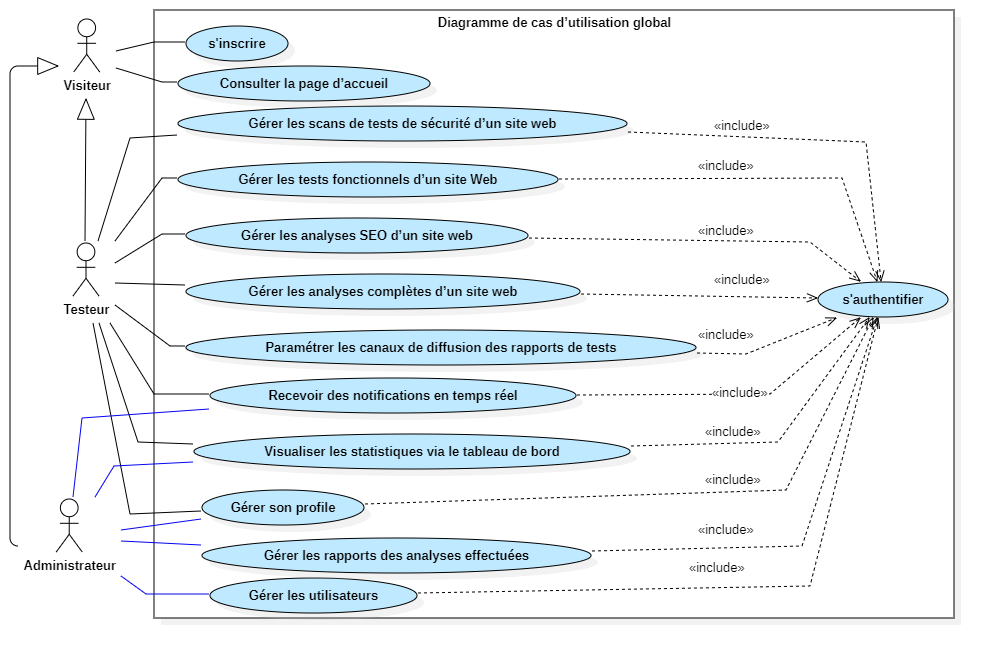
\includegraphics[width=\textwidth]{chapitres/ch2/img/global-last- use-case.png}
\caption{Diagramme de cas d'utilisation global}
\label{fig:UseCaseDiagram1}
\end{figure}
\vspace{-0.3cm}
    \section{Pilotage du projet avec Scrum}
    Cette section décrit le pilotage du projet selon la méthodologie Scrum, en présentant les outils utilisés, la composition de l’équipe et ses rôles, le backlog du produit et le découpage du projet.
\subsection{Présentation de l’équipe de travail }
La réussite du projet repose sur une bonne organisation de l’équipe et une répartition claire des rôles, assurées par la méthodologie Scrum. Dans le cadre de ce projet, les trois rôles clés de Scrum sont attribués aux membres de l’équipe de la manière suivante :
\begin{itemize}[label=$\bullet$]
    \item \textbf{Scrum Master:} Représenté par notre encadrant professionnel, Monsieur \textbf{Omar NACHMI}, qui a guidé l’équipe dans l’adoption de Scrum, assurant une organisation efficace et une amélioration continue des processus de travail.
    \item \textbf{Product Owner :}  Représenté également par Monsieur \textbf{Omar NACHMI}, qui a proposé et dirigé ce travail, en fournissant des explications approfondies sur les diverses exigences et fonctionnalités requises par le système.
    \item \textbf{Équipe de développement:} Composée de moi-même, \textbf{Rihab Cherni}, et de ma collègue \textbf{Maïssa Ben Ghalba}, nous avons travaillé ensemble pour réaliser le projet, en collaborant étroitement à chaque étape du développement.
\end{itemize}
\subsection{Outils SCRUM utilisés}
Pour le suivi de notre projet, nous avons adopté des outils collaboratifs : \textbf{OpenProject} pour la gestion des tâches et le suivi quotidien de notre progression, \textbf{Microsoft Teams} pour la communication entre les membres de l’équipe, l’organisation des réunions quotidiennes (daily meetings), des réunions RH et la coordination des sprints, et \textbf{GitLab} pour le travail collaboratif sur le code et la gestion de version.
 \subsection{Backlog du produit }
Le backlog produit représente une liste des fonctionnalités nécessaires au développement du produit. Géré par le Product Owner, il permet d'assurer l’alignement entre les besoins des utilisateurs et les objectifs du projet. Il constitue un outil de référence pour l’équipe de développement, en collaboration avec le Scrum Master et les parties prenantes \cite{backlog}.

Les epics structurent le backlog à un niveau stratégique en regroupant des fonctionnalités clés du produit. Plus génériques et moins détaillés que les user stories, ils doivent être découpés progressivement pour être développés. Ils facilitent la planification, la priorisation, la communication avec les parties prenantes et la gestion de la complexité tout au long du projet\cite{epic}.

Le tableau \ref{tab:backlog} présente le backlog produit de notre projet, en précisant pour chaque épique sa priorité, le niveau de risque, ainsi que son effort estimé en jours.
\renewcommand{\arraystretch}{1.3}
\begin{spacing}{1}
    \begin{longtable}{|p{0.35cm}|p{9.3cm}|p{1.45cm}|p{1.45cm}|p{2.4cm}|}
        \caption{Backlog produit} \label{tab:backlog} \\\hline
        \textbf{\small ID} & \textbf{\small Épics} & \textbf{\small Priorité} & \textbf{\small Risques} & \textbf{\small Estimation(j)} \\ \hline
        1  & \textbf{Initialisation du projet} & Élevée & Basse & 15 \\
        \hline
        2 & \textbf{Consultation de la page d’accueil} & Basse & Basse & 5 \\
        \hline 
        3  & \textbf{Authentification et gestion du profil} & Moyenne & Basse & 4 \\
        \hline
       4  & \textbf{Gestion des scans de tests de sécurité d’un site web} & Élevée & Élevée & 20 \\
        \hline  
        5  & \textbf{Gestion des tests fonctionnels d’un site web} & Élevée & Élevée & 15 \\
        \hline 
        6  & \textbf{Gestion des analyses SEO d’un site web} & Élevée & Moyenne & 10 \\
        \hline      
        7  & \textbf{Gestion des analyses complètes} & Élevée & Élevée & 6 \\
        \hline
        8  & \textbf{Visualisation des statistiques via le tableau de bord} & Élevée & Élevée & 8 \\
        \hline
        9  & \textbf{Notifications en temps réel} & Élevée & Basse & 2 \\
        \hline
        10 & \textbf{Paramétrage des canaux de diffusion des rapports de tests} & Moyenne & Moyenne & 2 \\ 
        \hline
        11 & \textbf{Gestion des utilisateurs} & Moyenne & Basse & 2 \\
        \hline
        12 & \textbf{Gestion des rapports des analyses effectuées } & Moyenne & Basse & 3 \\
        \hline
        13 & \textbf{Déploiement de l'application} & Moyenne & Moyenne & 5 \\
        \hline
        \multicolumn{4}{|c|}{\textbf{TOTAL}} & \textbf{97(jours)} \\
        \hline 
    \end{longtable}
\end{spacing}
\vspace{-0.1cm}
\subsection{Planification des sprints}
Pour la planification, nous avons choisi de répartir le travail en deux livraisons (releases), chacune étant divisée en deux sprints, comme indiqué dans le tableau \ref{tab:Planification}.
{\renewcommand{\arraystretch}{1.3}
\begin{table}[H]
	\begin{center}
    \caption{Planification des Livraisons et des Sprints}
    \label{tab:Planification}
	\begin{tabular}{|p{8.2cm}|p{8.2cm}|}\hline
		\textbf{Livraison 1 (Total : 50 jours)} & \textbf{Livraison 2 (Total : 47 jours)} \\\hline
		\begin{minipage}[t]{\linewidth}
            \textbf{Sprint 1.1} (26 jours) :
            \begin{itemize}[label=$-$, left=0.2cm]
                \item Initialisation du projet
                \item Consultation de la page d’accueil
                \item Authentification
                \item Gestion des utilisateurs
            \end{itemize}
            \textbf{Sprint 1.2} (24 jours) :
            \begin{itemize}[label=$-$, left=0.2cm]
                \item Gestion des scans de tests de sécurité
                \item Paramétrage des canaux de diffusion des rapports de tests
                \item Notifications en temps réel
            \end{itemize}
            \vspace{0.1cm}
        \end{minipage}
        &
        \begin{minipage}[t]{\linewidth}
            \textbf{Sprint 2.1} (25 jours) :
            \begin{itemize}[label=$-$, left=0.2cm]
                \item Gestion des scans fonctionnels
                \item Gestion des scans SEO
            \end{itemize}
            \textbf{Sprint 2.2} (22 jours) :
            \begin{itemize}[label=$-$, left=0.2cm]
                \item Gestion des scans complètes (fonctionnels, sécurité et SEO)
                \item Visualisation du tableau de bord
                \item Gestion des rapports des analyses effectuées
                \item Déploiement de l’application
            \end{itemize}
        \end{minipage}
        \\\hline
	\end{tabular}
 	\end{center}
\end{table}
}
\vspace{-0.7cm}
Cette répartition a permis d’ajuster le projet au fil des sprints tout en intégrant les fonctionnalités essentielles dès les premières étapes du développement. 
    \section{Planning prévisionnel du projet}
    Pour une gestion optimale du projet, nous avons utilisé un diagramme de Gantt, permettant de répartir les tâches de manière structurée et de visualiser leur durée ainsi que leur enchaînement. 
Comme illustré dans la figure \ref{fig:gantt}, chaque tâche est associée à un intervalle de temps précis, facilitant le suivi de l'avancement et la gestion des priorités. Cet outil aide à identifier les étapes clés et à ajuster les délais si nécessaire, garantissant ainsi une coordination efficace et un déroulement fluide du notre projet.
\begin{figure}[H]
    \centering
    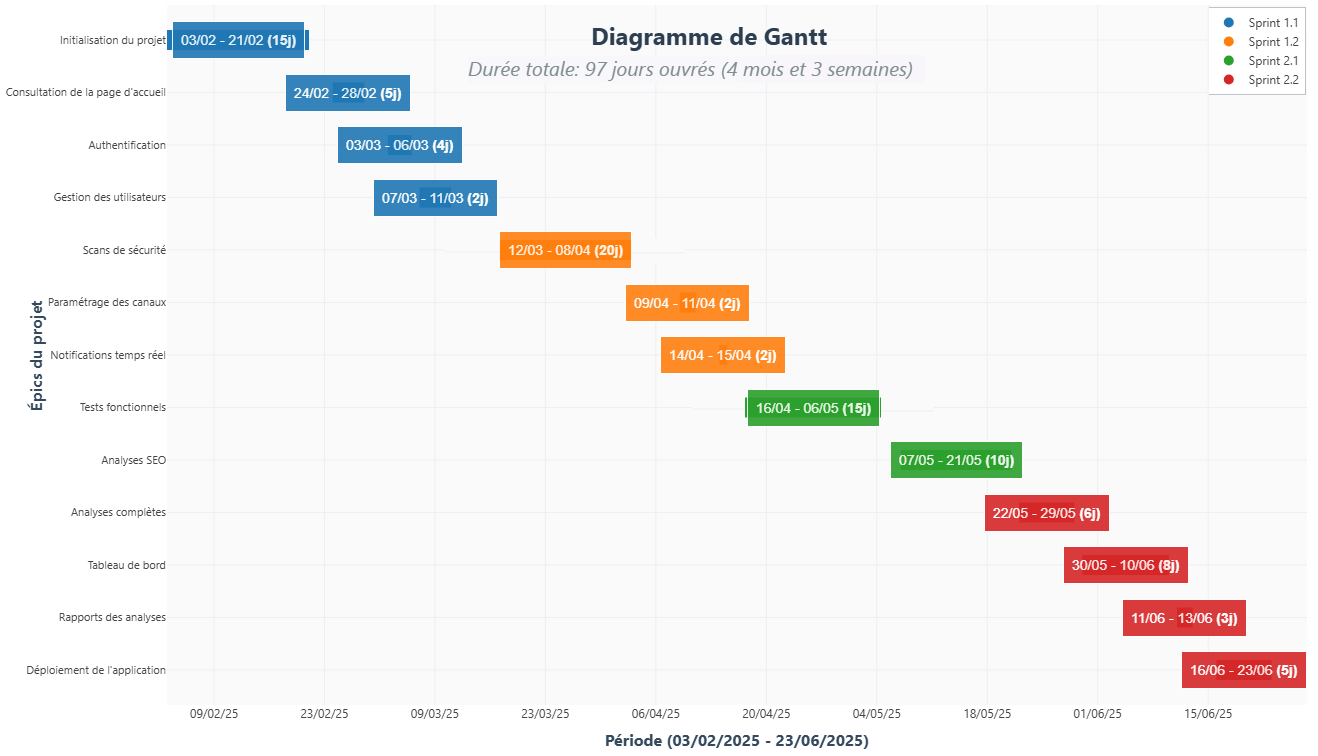
\includegraphics[width=\linewidth]{chapitres/ch2/img/gantt-last.png}
    \caption{Diagramme de Gantt}
    \label{fig:gantt}
\end{figure}
\vspace{-0.5cm}  
    \section{Rétrospective Agile}
    Dans cette section nous allons présenter les différents artefacts Scrum que nous avions utilisé pour accomplir notre projet afin de nous faciliter la gestion des tâches. 
\subsection{Scrum board}
Le Scrum board est un outil visuel utilisé pour organiser et suivre les tâches dans chaque sprint (à faire, en cours, terminées). Il permet aux équipes de suivre l'avancement du travail tout au long des sprints. Sa mise à jour est la responsabilité des membres de l’équipe, facilitant la gestion des tâches et la visualisation de la progression\cite{Scrumboard}.

Nous avons utilisé l’outil \textbf{«OpenProject»} pour organiser les tâches sous forme de cartes réparties sur quatre colonnes : à faire, en cours, à tester et terminées. Cet outil nous a permis de suivre efficacement l'avancement de nos sprints, comme illustré dans la figure \ref{fig:boardOpenProject} représentant le Scrum board du Sprint 1.
\begin{figure}[H]
    \centering
    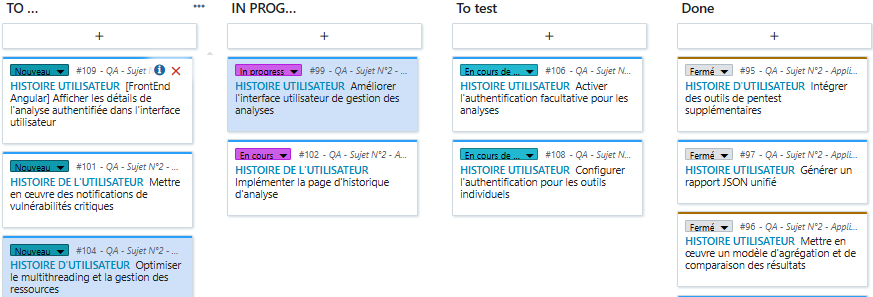
\includegraphics[width=\linewidth]{chapitres/ch2/img/board-sprit1.PNG}
    \caption{Scrum board Sprint 1}
    \label{fig:boardOpenProject}
\end{figure}
\vspace{-0.6cm}
\subsection{Burndown Chart}
Le Burndown Chart est un graphique visuel qui montre la quantité de travail terminée et celle restant à faire dans un sprint ou un projet, en fonction du temps écoulé. Il aide à estimer la capacité de l’équipe à atteindre ses objectifs dans les délais impartis et à détecter rapidement d’éventuelles dérives. La mise à jour régulière de ce graphique est essentielle pour anticiper les retards et ajuster le rythme de travail\cite{burndown}.

Nous avons généré les Burndown Charts à partir de l’avancement des tâches de chaque sprint. Ces graphiques nous ont permis de suivre efficacement notre progression et d’adapter notre charge de travail, comme illustré dans la figure \ref{fig:burndownChart} représentant le Burndown chart du projet.
\begin{figure}[H] 
    \centering 
    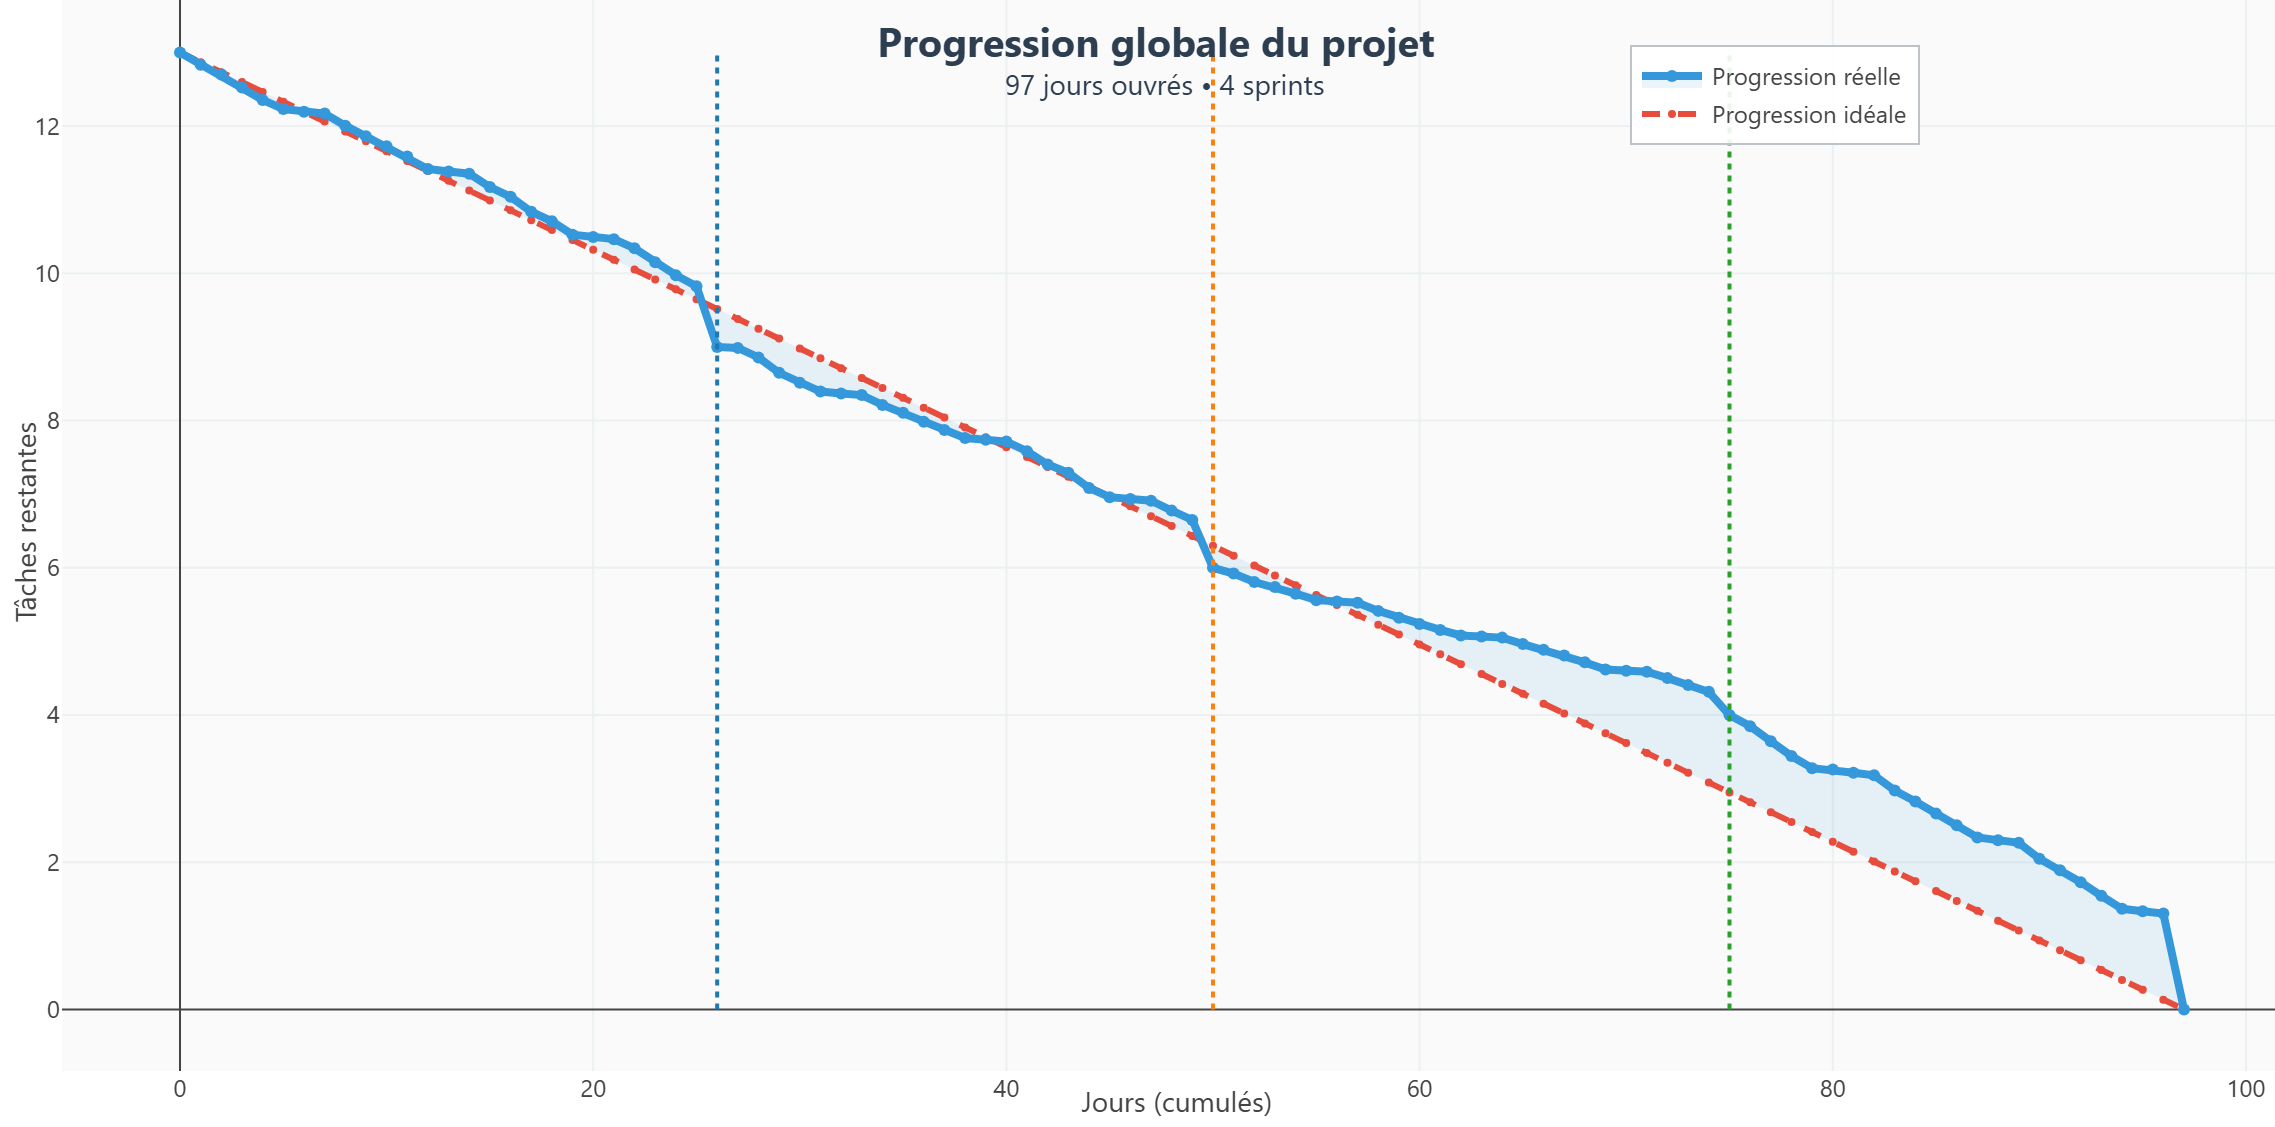
\includegraphics[width=0.97\linewidth]{chapitres/ch2/img/burndown.png} 
    \caption{Burndown chart projet} 
    \label{fig:burndownChart} \end{figure} 
\vspace{-0.8cm}
  
    \section{Environnement de développement}
    Cette section est dédiée pour la description de l’environnement matériel ainsi que l’environnement logiciel qui ont été employés pour la mise en œuvre de notre application
    \subsection{Environnement matériel}
    \begin{justify}
    Le tableau ~\ref{tab:environementMateriel} représente les caractéristiques techniques des machines utilisées pour la réalisation de notre application.
    \vspace{-0.5cm}
    \begin{table}[H]
        \begin{center}
        \renewcommand{\arraystretch}{1.5}
        \caption{Environnement matériel}
    	\begin{tabular}{|p{6cm}|p{8cm}|} 		
        	\hline				
        	\textbf{Type} & Ordinateur Portable\\\hline
            \textbf{Marque} & ASUS \\\hline
            \textbf{Processeur}  & Intel Core i5\\\hline
            \textbf{RAM} & 12 Go  \\ \hline
            \textbf{Disque dur} & 256 Go SSD\\\hline
            \textbf{Système d’exploitation}  & Windows 10 (64 bits)\\\hline
	      \end{tabular}
            \label{tab:environementMateriel}
        \end{center}
    \end{table}
\end{justify}
    \vspace{-0.5cm}
    \subsection{Environnement logiciel}
    \begin{justify}
    Pour la réalisation de notre application, plusieurs outils logiciels ont été utilisés, incluant les environnements de développement, les bibliothèques, les frameworks, ainsi que des outils et des services externes. Cette section présente une description de ces éléments.
    \subsubsection{Langages utilisés}
        Les langages présentés dans le tableau~\ref{tab:Langages} ont été utilisés pour développer les différentes composantes de l'application.
        \vspace{-0.3cm}
        \begin{spacing}{1.2}
            \begin{longtable}{|c|p{0.75\textwidth}|}
                \caption{Langages utilisés}
                \label{tab:Langages}\\
                \hline
                \textbf{Langage} & \textbf{Description} \\ \hline
                
                %% Python
                \begin{minipage}{0.2\textwidth}
                \centering
                    
\includegraphics[width=2cm]{chapitres/ch2/img/logiciel/python.png}
                \end{minipage}
                 & \begin{minipage}{0.75\textwidth} 
                  \justifying
                \vspace{0.2cm}
                \textbf{Python} est utilisé pour le développement du backend avec le framework \textbf{FastAPI}. Ce langage est reconnu pour sa lisibilité et sa simplicité, ce qui facilite la création d'API REST performantes et évolutives\cite{python}.
                \vspace{0.2cm}
                \end{minipage}\\ \hline
                
                %% TypeScript
                \begin{minipage}{0.2\textwidth}
                \centering
                    
\includegraphics[width=1.8cm]{chapitres/ch2/img/logiciel/ts.png}
                \end{minipage}
                 & \begin{minipage}{0.75\textwidth} 
                  \justifying
                \vspace{0.2cm}
                \textbf{TypeScript} est un sur-ensemble typé de JavaScript utilisé dans le développement de l'interface utilisateur via le framework \textbf{Angular}. Il permet de sécuriser le code et d'améliorer la maintenabilité des composants frontend\cite{typescript}.
                \vspace{0.2cm}
                \end{minipage}\\ \hline
    
                %% HTML
                \begin{minipage}{0.2\textwidth}
                \centering
                
\includegraphics[width=2cm]{chapitres/ch2/img/logiciel/html.png}
                \end{minipage}
                & \begin{minipage}{0.75\textwidth} 
                \justifying
                \vspace{0.2cm}
                \textbf{HTML (HyperText Markup Language)} est le langage standard utilisé pour structurer les pages web. Il définit les éléments de base tels que les titres, paragraphes, liens, tableaux, formulaires, etc.\cite{html}.
                \vspace{0.2cm}
                \end{minipage}\\ \hline
                
                %% CSS
                \begin{minipage}{0.2\textwidth}
                \centering
                
\includegraphics[width=2cm]{chapitres/ch2/img/logiciel/css.png}
                \end{minipage}
                & \begin{minipage}{0.75\textwidth} 
                \justifying
                \vspace{0.2cm}
                \textbf{CSS (Cascading Style Sheets)} est utilisé pour styliser les éléments HTML. Il permet de définir l'apparence des pages (couleurs, polices, marges, positionnement, etc.) afin d'améliorer l'expérience utilisateur\cite{css}.
                \vspace{0.2cm}
                \end{minipage}\\ \hline
                            %% SQL (PostgreSQL)
                \begin{minipage}{0.2\textwidth}
                    \centering
                        
\includegraphics[width=2cm]{chapitres/ch2/img/logiciel/sql.jpg}
                \end{minipage}
                 & \begin{minipage}{0.75\textwidth} 
                      \justifying
                        \vspace{0.2cm}
                        \textbf{SQL} est utilisé pour la gestion de la base de données relationnelle via le système \textbf{PostgreSQL}. Il permet de créer, manipuler et interroger les données de manière structurée\cite{postgresql}.
                        \vspace{0.2cm}
                \end{minipage}\\ \hline
                %% YAML
                \begin{minipage}{0.2\textwidth}
                    \centering
                        
\includegraphics[width=2cm]{chapitres/ch2/img/logiciel/yaml.png}
                \end{minipage}
                 & \begin{minipage}{0.75\textwidth} 
                    \justifying
                    \vspace{0.2cm}
                    \textbf{YAML} est utilisé pour la configuration des conteneurs dans \textbf{Docker Compose}. Il permet de définir les services, les volumes, les ports et les dépendances nécessaires au déploiement de l’application\cite{yaml}.
                    \vspace{0.2cm}
                \end{minipage}\\ \hline
                
                %% JSON
                \begin{minipage}{0.2\textwidth}
                    \centering
                        
\includegraphics[width=2cm]{chapitres/ch2/img/logiciel/json.jpg}
                \end{minipage}
                 & \begin{minipage}{0.75\textwidth} 
                    \justifying
                    \vspace{0.2cm}
                    \textbf{JSON (JavaScript Object Notation)} est utilisé comme format d'échange de données entre le frontend Angular et le backend FastAPI, ainsi que pour la documentation des API via Swagger/OpenAPI\cite{json}.
                    \vspace{0.2cm}
                \end{minipage}\\ \hline
                %% Bash
                \begin{minipage}{0.2\textwidth}
                    \centering
                        
\includegraphics[width=2cm]{chapitres/ch2/img/logiciel/bash.png}
                \end{minipage}
                 & \begin{minipage}{0.75\textwidth} 
                    \justifying
                    \vspace{0.2cm}
                    \textbf{Bash} est utilisé pour automatiser l'exécution de scripts liés aux tests de sécurité, au déploiement des conteneurs Docker, à la gestion des dépendances, et à l'enchaînement des outils d’analyse\cite{bash}.
                    \vspace{0.2cm}
                \end{minipage}\\ \hline
            \end{longtable}
        \end{spacing}
    \vspace{-0.2cm}
    \subsubsection{Logiciels utilisés}
    Le tableau~\ref{tab:Logiciels} présente un récapitulatif des outils employés pour la mise en œuvre de la solution ainsi que leurs descriptions.
    \vspace{-0.2cm}
            \begin{spacing}{1.1}
                \begin{longtable}{|c|p{0.75\textwidth}|}
                   \caption{Logiciels utilisés}
                    \label{tab:Logiciels}\\
                    \hline
                    \textbf{Logiciel} & \textbf{Description} \\ \hline
                    %% VS Code
                    \begin{minipage}{0.2\textwidth}
                    \centering
                        
\includegraphics[width=2.2cm]{chapitres/ch2/img/logiciel/vscode.png}
                    \end{minipage}
                     & \begin{minipage}{0.75\textwidth} 
                      \justifying
                    \vspace{0.2cm}
                    \textbf{Visual Studio Code (VS Code)} est un éditeur de code source open-source de Microsoft, réputé pour sa polyvalence, sa légèreté et ses fonctionnalités avancées. Il offre un environnement extensible grâce à des extensions, ce qui simplifie le travail des programmeurs\cite{VisualStudioCode}.\vspace{0.2cm}
                    \end{minipage}\\ \hline
                    %% GitHub
                    \begin{minipage}{0.2\textwidth}
                    \centering
                        
\includegraphics[width=3.2cm]{chapitres/ch2/img/logiciel/gitlab.png}
                    \end{minipage}
                     & \begin{minipage}{0.75\textwidth}
                      \justifying
                    \vspace{0.2cm}
                        \textbf{Gitlab} est une plateforme DevOps open source qui centralise le cycle de vie des projets logiciels : gestion de code, CI/CD, gestion de projet et sécurité. Elle favorise la collaboration, l’automatisation et la traçabilité, permettant aux équipes de planifier, développer, tester et déployer plus efficacement. Grâce à sa richesse fonctionnelle, elle s’impose comme un outil essentiel du développement moderne\cite{gitlab}.
                    \vspace{0.2cm}
                    \end{minipage}\\ \hline
                    %% Git
                    \begin{minipage}{0.2\textwidth}
                    \centering
                        
\includegraphics[width=2.1cm]{chapitres/ch2/img/logiciel/git.png}
                    \end{minipage}
                     & \begin{minipage}{0.75\textwidth} 
                     \justifying
                    \vspace{0.2cm}
                        \textbf{Git} permet la gestion efficace des branches pour travailler simultanément sur plusieurs projets sans conflits, en offrant une interface console conviviale, des algorithmes de fusion intelligents pour gérer les modifications simultanées de fichiers\cite{git}.
                    \vspace{0.2cm}
                    \end{minipage}\\ \hline
                    %% Docker Desktop
                    \begin{minipage}{0.2\textwidth}
                    \centering
                        
\includegraphics[width=2.6cm]{chapitres/ch2/img/logiciel/Docker Desktop.png}
                    \end{minipage}
                     & \begin{minipage}{0.75\textwidth} 
                      \justifying
                    \vspace{0.2cm}
                    \textbf{Docker Desktop} est une application pour Windows, macOS et Linux qui fournit une interface utilisateur graphique (GUI) pour gérer les conteneurs, images et réseaux Docker localement. Elle inclut Docker Engine, Docker CLI, Docker Compose, Kubernetes et d'autres outils utiles pour le développement et le test de conteneurs\cite{dockerdesktop}.
                    \vspace{0.2cm}
                    \end{minipage}\\ \hline
                    %% WebSocket
                    \begin{minipage}{0.2\textwidth}
                    \centering
                        
\includegraphics[width=2cm]{chapitres/ch2/img/logiciel/websocket.png}
                    \end{minipage}
                     & \begin{minipage}{0.75\textwidth} 
                      \justifying
                    \vspace{0.2cm}
                    \textbf{WebSocket} est un protocole de communication bidirectionnelle full-duplex permettant des échanges en temps réel entre client et serveur. Il est utilisé pour transmettre en direct les résultats des scans et notifier l’utilisateur via l’interface Angular\cite{websocket}.
                    \vspace{0.2cm}
                    \end{minipage}\\ \hline
                    %% Overleaf
                    \begin{minipage}{0.2\textwidth}
                    \vspace{0.2cm}
                    \centering
                        
\includegraphics[width=2.2cm]{chapitres/ch2/img/logiciel/overleaf.png}
                    \end{minipage}
                     & \begin{minipage}{0.75\textwidth}
                      \justifying
                    \vspace{0.2cm}
                         \textbf{Overleaf} est une plateforme en ligne de rédaction collaborative en temps réel de documents LaTeX, conçue pour la création de documents scientifiques, académiques et techniques\cite{Overleaf}.
                    \vspace{0.2cm}
                    \end{minipage}\\ \hline
                    %% StarUML
                    \begin{minipage}{0.2\textwidth}
                    \centering
                        \includegraphics[width=1.9cm]{chapitres/ch2/img/logiciel/staruml.png}
                    \end{minipage}
                     & \begin{minipage}{0.75\textwidth} 
                      \justifying
                    \vspace{0.2cm}
                         \textbf{StarUML} est un logiciel de modélisation UML utilisé pour concevoir des diagrammes pour la conception de logiciels. Il offre des fonctionnalités de modélisation avancées pour les concepteurs de logiciels\cite{StarUML}. \vspace{0.2cm}
                    \end{minipage}\\ \hline
                    %% Trello
                    \begin{minipage}{0.2\textwidth}
                    \centering
                        \includegraphics[width=3cm]{chapitres/ch2/img/logiciel/openproject.png}
                    \end{minipage}
                     & \begin{minipage}{0.75\textwidth}
                      \justifying
                        \vspace{0.2cm}
                         \textbf{OpenProject} est un logiciel de gestion de projet open source conçu pour être utilisé avec des méthodologies de gestion de projet traditionnelles, mais aussi dans un environnement agile ou une méthodologie hybride. Collaboratif, il offre un suivi de projet et une suite complète de fonctionnalités permettant de gérer des projets complexes\cite{openproject}.
                    \vspace{0.2cm}
                    \end{minipage}\\ \hline
                    %% Postman
                    \begin{minipage}{0.2\textwidth}
                    \centering
                        \includegraphics[width=2.2cm]{chapitres/ch2/img/logiciel/postman.png}
                    \end{minipage}
                     & \begin{minipage}{0.75\textwidth} 
                      \justifying
                    \vspace{0.2cm}
                         \textbf{Postman} est un outil de développement d'API qui permet aux développeurs de tester, de documenter et de surveiller les API de manière efficace. Il offre une interface conviviale pour créer des requêtes HTTP, automatiser des tests et collaborer sur des projets d'API \cite{Postman}.
                    \vspace{0.2cm}
                    \end{minipage}\\ \hline
            
            
                    \begin{minipage}{0.2\textwidth}
                    \centering
                        \includegraphics[width=2.2cm]{chapitres/ch2/img/logiciel/Swagger.png}
                    \end{minipage}
                     & \begin{minipage}{0.75\textwidth} 
                      \justifying
                    \vspace{0.2cm}
                        \textbf{Swagger} est un langage de description d’interface permettant de définir des API REST à l’aide du format JSON. Il s’appuie sur la spécification OpenAPI, qui standardise la description de la structure d’une API. Il permet de concevoir, documenter, tester et consommer des API REST facilitant ainsi la compréhension et l’intégration des services web\cite{Swagger}.
                    \vspace{0.2cm}
                    \end{minipage}\\ \hline
            
                \begin{minipage}{0.2\textwidth}
                    \centering
                        \includegraphics[width=2.2cm]{chapitres/ch2/img/logiciel/Selenium.png}
                    \end{minipage}
                     & \begin{minipage}{0.75\textwidth} 
                      \justifying
                    \vspace{0.2cm}
                        \textbf{Selenium} est un outil open-source largement utilisé pour l'automatisation des tests des applications web. Il permet d'écrire des scripts de test dans divers langages de programmation comme Java, Python, C\#. Il permet de simuler des interactions utilisateur telles que les clics, la saisie de texte et la navigation entre les pages, ce qui est essentiel pour les tests fonctionnels des applications web.\cite{selenium}.
                    \vspace{0.2cm}
                    \end{minipage}\\ \hline
                \end{longtable}
            \end{spacing}
            \vspace{-0.1cm}
    \subsubsection{ Frameworks utilisées}
    Le tableau~\ref{tab:Libs} présente les principales  frameworks utilisées dans le développement de l'application, réparties entre le backend et le frontend. Ces  frameworks  ont permis de faciliter le développement, d'améliorer les performances et de garantir la sécurité et la maintenabilité du projet.
    \begin{spacing}{1.1}
        \begin{longtable}{|c|p{0.75\textwidth}|}
            \caption{Bibliothèques utilisées}
            \label{tab:Libs}\\
            \hline
            \textbf{Bibliothèque} & \textbf{Description} \\ \hline
            
            %% FastAPI
            \begin{minipage}{0.2\textwidth}
                \centering
                    \includegraphics[width=1.9cm]{chapitres/ch2/img/logiciel/fastapi.png}
            \end{minipage}
             & \begin{minipage}{0.75\textwidth} 
                \justifying
                \vspace{0.2cm}
                \textbf{FastAPI} est une bibliothèque Python moderne permettant de créer des API web de manière rapide, performante et avec une documentation automatique générée via OpenAPI/Swagger\cite{fastapi}.
                \vspace{0.2cm}
            \end{minipage}\\ \hline
            
            %% Angular 
            \begin{minipage}{0.2\textwidth}
                \centering
                    \includegraphics[width=2.6cm]{chapitres/ch2/img/logiciel/angular.png}
            \end{minipage}
             & \begin{minipage}{0.75\textwidth} 
                    \justifying
                    \vspace{0.2cm}
                    \textbf{Angular} est un framework de développement frontend basé sur TypeScript, utilisé pour concevoir des applications web dynamiques, modulaires et performantes. Il propose une architecture robuste fondée sur des composants, un système de routage, des formulaires réactifs ainsi qu’une gestion d’état, facilitant le développement d’interfaces utilisateur complexes \cite{angular}.
                    \vspace{0.1cm}
            \end{minipage}\\ \hline
            
            %% Bootstrap
            \begin{minipage}{0.2\textwidth}
                \centering
                \includegraphics[width=2cm]{chapitres/ch2/img/logiciel/bootstrap.jpg}
                \end{minipage}
                & \begin{minipage}{0.75\textwidth} 
                \justifying
                \vspace{0.2cm}
                \textbf{Bootstrap} est une bibliothèque CSS open-source qui facilite le développement de sites web réactifs. Elle fournit des composants préconçus (boutons, cartes, grilles) et garantit une compatibilité multi-appareils\cite{bootstrap}.
                \vspace{0.2cm}
                \end{minipage}\\ \hline
            \end{longtable}
        \end{spacing}
    \vspace{-0.1cm}
    \subsubsection{Outils de sécurité utilisés}
    Le tableau~\ref{tab:OutilsSecurite} présente les outils de sécurité employés pour les tests de vulnérabilités et l'analyse de sécurité de l'application.
    \begin{spacing}{1.1}
        \begin{longtable}{|c|p{0.75\textwidth}|}
            \caption{Outils de sécurité utilisés}
            \label{tab:OutilsSecurite}\\
            \hline
            \textbf{Outil} & \textbf{Description} \\ \hline
            
            %% ZAP
            \begin{minipage}{0.2\textwidth}
                \centering
                    \includegraphics[width=2.4cm]{chapitres/ch2/img/tools/zap.png}
            \end{minipage}
             & \begin{minipage}{0.75\textwidth} 
                \justifying
                \vspace{0.2cm}
                \textbf{ZAP (OWASP Zed Attack Proxy)} est un outil open-source de test de sécurité des applications web. Il permet de détecter automatiquement les vulnérabilités courantes telles que les failles XSS (Cross-Site Scripting), CSRF (Cross-Site Request Forgery), et les injections SQL dans les applications web\cite{zap}.
                \vspace{0.2cm}
            \end{minipage}\\ \hline
            
            %% SQLMap
            \begin{minipage}{0.2\textwidth}
                \centering
                    \includegraphics[width=3.4cm]{chapitres/ch2/img/tools/sqlmap.png}
            \end{minipage}
             & \begin{minipage}{0.75\textwidth} 
                \justifying
                \vspace{0.2cm}
                \textbf{SQLMap} est un outil automatisé open-source spécialisé dans la détection et l'exploitation des vulnérabilités d'injection SQL. Il prend en charge de nombreux systèmes de gestion de bases de données et offre des techniques avancées pour l'extraction de données et la prise de contrôle des bases de données vulnérables\cite{sqlmap}.
                \vspace{0.2cm}
            \end{minipage}\\ \hline
            
            %% Wapiti
            \begin{minipage}{0.2\textwidth}
                \centering
                    \includegraphics[width=2.8cm]{chapitres/ch2/img/tools/wapiti.png}
            \end{minipage}
             & \begin{minipage}{0.75\textwidth} 
                \justifying
                \vspace{0.2cm}
                \textbf{Wapiti} est un scanner de vulnérabilités web open-source qui effectue des audits de sécurité en analysant les pages web pour détecter les scripts et les formulaires où il pourrait injecter des données. Il permet d'identifier diverses vulnérabilités comme les injections SQL, XSS, et les inclusions de fichiers\cite{wapiti}.
                \vspace{0.2cm}
            \end{minipage}\\ \hline
            
            %% Nikto
            \begin{minipage}{0.2\textwidth}
                \centering
                    \includegraphics[width=2.4cm]{chapitres/ch2/img/tools/nikto.png}
            \end{minipage}
             & \begin{minipage}{0.75\textwidth} 
                \justifying
                \vspace{0.2cm}
                \textbf{Nikto} est un scanner de vulnérabilités web open-source qui effectue des tests complets contre les serveurs web pour multiple vulnérabilités, incluant plus de 6700 fichiers/programmes potentiellement dangereux, les versions obsolètes de serveurs, et les problèmes de configuration spécifiques aux serveurs\cite{nikto}.
                \vspace{0.2cm}
            \end{minipage}\\ \hline
            
            %% Nuclei
            \begin{minipage}{0.2\textwidth}
                \centering
                    \includegraphics[width=3.2cm]{chapitres/ch2/img/tools/nuclei.png}
            \end{minipage}
             & \begin{minipage}{0.75\textwidth} 
                \justifying
                \vspace{0.2cm}
                \textbf{Nuclei} est un scanner de vulnérabilités rapide et personnalisable basé sur des templates YAML. Il permet d'effectuer des scans de sécurité à grande échelle avec une approche modulaire, supportant la détection de diverses vulnérabilités web, réseau et cloud\cite{nuclei}.
                \vspace{0.2cm}
            \end{minipage}\\ \hline
            
            %% Nmap
            \begin{minipage}{0.2\textwidth}
                \centering
                    \includegraphics[width=2.8cm]{chapitres/ch2/img/tools/nmap.png}
            \end{minipage}
             & \begin{minipage}{0.75\textwidth} 
                \justifying
                \vspace{0.2cm}
                \textbf{Nmap (Network Mapper)} est un outil open-source de découverte réseau et d'audit de sécurité. Il permet de scanner les ports ouverts, identifier les services en cours d'exécution, détecter les systèmes d'exploitation, et effectuer des scripts de reconnaissance avancés sur les réseaux\cite{nmap}.
                \vspace{0.2cm}
            \end{minipage}\\ \hline
            
            %% XSStrike
            \begin{minipage}{0.2\textwidth}
                \centering
                    \includegraphics[width=2.4cm]{chapitres/ch2/img/tools/XSStrike.png}
            \end{minipage}
             & \begin{minipage}{0.75\textwidth} 
                \justifying
                \vspace{0.2cm}
                \textbf{XSStrike} est un outil avancé de détection des vulnérabilités Cross-Site Scripting (XSS). Il utilise des techniques de fuzzing intelligentes et une analyse contextuelle pour identifier les failles XSS complexes que les scanners traditionnels pourraient manquer\cite{xsstrike}.
                \vspace{0.2cm}
            \end{minipage}\\ \hline
            
            %% PwnXSS
            \begin{minipage}{0.2\textwidth}
                \centering
                    \includegraphics[width=3.6cm]{chapitres/ch2/img/tools/PwnXSS.png}
            \end{minipage}
             & \begin{minipage}{0.75\textwidth} 
                \justifying
                \vspace{0.2cm}
                \textbf{PwnXSS} est un outil spécialisé dans la détection avancée des vulnérabilités Cross-Site Scripting. Il offre des capacités de scanning automatisé avec des payloads personnalisés et une analyse approfondie des réponses pour identifier les failles XSS dans diverses configurations d'applications web\cite{pwnxss}.
                \vspace{0.2cm}
            \end{minipage}\\ \hline
            
            %% WafW00f
            \begin{minipage}{0.2\textwidth}
                \centering
                    \includegraphics[width=2.4cm]{chapitres/ch2/img/tools/wafw00f.png}
            \end{minipage}
             & \begin{minipage}{0.75\textwidth} 
                \justifying
                \vspace{0.2cm}
                \textbf{WafW00f} est un outil Python conçu pour identifier et fingerprinter les Web Application Firewalls (WAF) protégeant une application web. Il permet aux testeurs de sécurité de déterminer la présence et le type de WAF afin d'adapter leurs stratégies de test en conséquence\cite{wafw00f}.
                \vspace{0.2cm}
            \end{minipage}\\ \hline
            
            %% WhatWeb
            \begin{minipage}{0.2\textwidth}
                \centering
                    \includegraphics[width=3.6cm]{chapitres/ch2/img/tools/Whatweb.png}
            \end{minipage}
             & \begin{minipage}{0.75\textwidth} 
                \justifying
                \vspace{0.2cm}
                \textbf{WhatWeb} est un outil de reconnaissance web qui identifie les technologies utilisées par un site web, incluant les systèmes de gestion de contenu, les frameworks, les serveurs web, les bibliothèques JavaScript, et d'autres composants technologiques. Il est essentiel pour le fingerprinting et la reconnaissance passive\cite{whatweb}.
                \vspace{0.2cm}
            \end{minipage}\\ \hline
        \end{longtable}
    \end{spacing}
    \vspace{-0.1cm}
    \subsubsection{Système de gestion de base de données : PostgreSQL}
        \begin{minipage}{0.25\textwidth}
            \centering
            \includegraphics[width=3cm]{chapitres/ch2/img/logiciel/postgresql.png}
        \end{minipage}
        \begin{minipage}{0.75\textwidth} 
            \justifying
            \textbf{PostgreSQL} est un système de gestion de base de données relationnelle (SGBDR) open-source reconnu pour sa robustesse, sa conformité aux standards SQL, et son extensibilité. Il est utilisé pour stocker les données de manière fiable, en assurant l'intégrité des transactions, la cohérence et la sécurité des informations.
        \end{minipage}
        
        Dans notre application, PostgreSQL permet de gérer les entités principales telles que les utilisateurs, les messages, les enregistrements de données, etc. Il est accédé via SQLAlchemy, un ORM Python, facilitant les interactions entre les objets du backend (FastAPI) et la base de données.
    \subsubsection{Système de gestion des files de messages : RabbitMQ}
        \begin{minipage}{0.25\textwidth}
            \centering
            \includegraphics[width=3cm]{chapitres/ch2/img/logiciel/rabbitmq.png}
        \end{minipage}
        \begin{minipage}{0.75\textwidth} 
            \justifying
            \textbf{RabbitMQ} est un broker de messages open-source basé sur le protocole AMQP, permettant une communication asynchrone entre microservices et composants distribués. Il facilite le traitement parallèle ainsi que la gestion des files d’attente dans l’architecture backend \cite{rabbitmq}.
        \end{minipage}
        
        Dans notre application, RabbitMQ gère la mise en file d’attente des tâches de scans de sécurité afin d’améliorer les performances en limitant le nombre de scans exécutés simultanément et en évitant la surcharge des ressources. Les requêtes de scan sont placées dans des queues puis consommées par des workers dédiés, ce qui garantit une exécution efficace, fiable et scalable. Cette architecture favorise la tolérance aux pannes, le traitement asynchrone et l’extensibilité future. L’intégration s’appuie sur la bibliothèque Python \texttt{pika}, connectée au backend FastAPI, qui orchestre la production et la consommation des messages. Ainsi, les producteurs (backend FastAPI) envoient les requêtes de scan vers RabbitMQ, tandis que les consommateurs (workers) traitent ces messages en parallèle, optimisant la gestion de la charge et les performances.
\end{justify} 
    \section{Architecture de l’application}
    Cette section présente l’architecture de notre solution, conçue pour garantir la cohérence, la performance, la maintenabilité et la scalabilité de l’application. Elle repose sur une architecture en trois tiers, typique des applications web modernes, intégrant des services conteneurisés et orchestrés afin d’optimiser le développement, le déploiement et l’exécution.

L’architecture s’articule autour de trois couches principales:
\begin{itemize}[label=$-$]
    \item \textbf{Couche de présentation (Frontend)}: développée avec \textbf{Angular} (version 18), cette couche constitue l’interface utilisateur accessible via un navigateur web, sur le port \textbf{4200}. L’application est conteneurisée à l’aide de \textbf{Docker} et servie par un serveur web \textbf{NGINX} sur le port \textbf{80}, garantissant rapidité et sécurité côté client. Elle suit le modèle \textbf{\acs{MVVM}} (Model-View-ViewModel)\cite{mvvm}:
            \begin{itemize}[label=$\circ$]
                    \item \textbf{Model}: définit les structures de données via des interfaces \texttt{TypeScript}, représentant les entités métier (utilisateurs, scans, résultats...).
                    \item \textbf{View}: composants visuels construits en \texttt{HTML}/\texttt{CSS}, correspondant à la partie graphique de l’application.
                    \item \textbf{ViewModel}: représenté par les \textbf{Components} Angular (liaison entre données et vue) et les \textbf{Services} (logique métier côté client, communication avec le backend).
            \end{itemize}
        En complément, le frontend s’appuie sur plusieurs mécanismes clés assurant la sécurité, la modularité et l’interactivité de l’application:
        \begin{itemize}[label=$\circ$]
            \item \textbf{Guards et routing Angular}: sécurisent la navigation à travers un système de routes hiérarchisées, protégées selon l’état d’authentification et le rôle de l’utilisateur.
            \item \textbf{Services Angular}: centralisent les interactions avec l’API REST (via \texttt{HttpClient}) et les traitements locaux (authentification, stockage, notifications, WebSocket).
            \item \textbf{Modèles TypeScript}: définissent les formats d’échange avec le backend, alignés avec les schémas \texttt{Pydantic} de FastAPI, pour faciliter la sérialisation/désérialisation des données.
            \item \textbf{WebSocket}: permet une communication bidirectionnelle en temps réel pour recevoir les mises à jour instantanées (progression des scans, alertes système).
        \end{itemize}
    \item \textbf{Couche applicative (Backend)}: développée avec \textbf{FastAPI}, elle est accessible via le port \textbf{8000} pour les requêtes \acs{HTTP}, et le port \textbf{8001} pour les communications \textbf{WebSocket}. Elle assure la logique métier, le traitement des requêtes, l’exposition des services web REST, l’interfaçage avec la base de données, la gestion de l’authentification et la coordination entre les autres couches.
    L’application est conteneurisée à l’aide de \textbf{Docker} et déployée via un \textbf{serveur Uvicorn} conforme à l’interface \textbf{\acs{ASGI}}, utilisé pour exécuter l’application \textbf{FastAPI}. Ce serveur gère efficacement les requêtes \acs{HTTP}/\acs{HTTPS} et les transmet aux routes définies dans FastAPI. Il prend également en charge les communications asynchrones via les \textbf{WebSockets}, ce qui le rend particulièrement adapté aux applications modernes nécessitant des échanges en temps réel.
    \begin{enumerate}[left=-0.03cm]
        \item \textbf{Les composants principaux de fastapi sont\cite{fastapiArc}}:
            \begin{itemize}[label=$\bullet$, left=-0.08cm]
                \item \textbf{Routes:} définissent les points d'entrée de l'\acs{API} REST, organisés par fonctionnalité et reçoivent les requêtes \acs{HTTP}.
                \item \textbf{CRUD}: Contiennent la logique métier et le traitement des données.
                \item \textbf{Models:} représentent les entités de la base de données sous forme de classes SQLAlchemy (\acs{ORM}).
                \item \textbf{Schemas Pydantic:} utilisés pour la validation et la sérialisation des données, ils définissent la structure des informations échangées (requêtes et réponses) entre le client et l’API.
                \item \textbf{\acs{DAO} (Data Access Objects)}: basé sur \textbf{SQLAlchemy} pour accéder à la base de données PostgreSQL, en assurant le mapping objet-relationnel (ORM).
                \item \textbf{JWT / OAuth2:} mécanisme d’authentification sécurisé reposant sur l’utilisation de \textbf{\acs{JWT}} (JSON Web Tokens) en combinaison avec le protocole \textbf{\acs{OAuth2}}, permettant la gestion des sessions, le contrôle des accès et l’attribution des rôles utilisateurs.
                \item \textbf{Canal WebSocket}: utilisé pour la communication en temps réel avec les utilisateurs, il permet à ces derniers de recevoir des mises à jour instantanées (notifications, état des scans, messages système...).
            \end{itemize}
        \item \textbf{Composants spécifiques ajoutés pour ce projet:}
            \begin{itemize}[label=$\bullet$, left=-0.08cm]
                \item \textbf{File de messages RabbitMQ + Workers}: fonctionne sur le port \textbf{5672} (port par défaut pour le protocole \acs{AMQP}) et expose une interface d’administration sur le port \textbf{15672}. Ce système permet le traitement asynchrone des tâches lourdes, telles que la gestion des scans, en répartissant la charge entre un pool de \textbf{workers asynchrones}. Les requêtes sont placées dans une file d’attente, puis traitées selon un nombre limité de tâches concurrentes afin de garantir les performances et la stabilité du système.\\
                Ce mécanisme permet de:
                \begin{itemize}[label=$\circ$]
                    \item Enregistrer les requêtes de scan dans RabbitMQ.
                    \item Traiter les tâches de façon asynchrone via un nombre fixe de \textbf{workers}.
                    \item Garantir une répartition équitable des ressources (N scans simultanés maximum).
                    \item Notifier l’utilisateur en temps réel une fois le traitement terminé.
                \end{itemize}
                Il favorise ainsi la scalabilité et prévient la saturation du système.
                \item \textbf{Service \acs{SMTP}}: utilisé pour l’envoi d’e-mails via le port \textbf{587} (TLS), selon la configuration du serveur SMTP.
                \item \textbf{Intégration \acs{Slack}}: notifications automatiques envoyées sur un canal Slack configuré via Webhook pour informer en temps réel des événements critiques (début/fin de scan, erreurs, vulnérabilités détectées).
                \item \textbf{Intégration Jira}: création automatique de tickets dans Jira lors de la détection de vulnérabilités critiques ou bloquantes, avec transmission des détails techniques (type, niveau de risque, description, solution proposée) depuis le backend.
               \item \textbf{Outils de sécurité}: L’application intègre plusieurs outils de scan automatisé, chacun exécuté dans un conteneur \textbf{Docker} isolé afin de garantir la modularité et l’évolutivité. Parmi ces outils, OWASP ZAP est accessible via le port \textbf{8080}, utilisé pour l’API et le proxy web. Les autres outils SQLMap, Wapiti, Nikto, Nuclei, Nmap, XSStrike, PwnXSS, WafW00f et WhatWeb sont lancés via des commandes dans leurs conteneurs Docker respectifs, sans ports exposés, car ils ne fonctionnent pas comme des services persistants. Les résultats sont ensuite centralisés, structurés et unifiés afin de pouvoir être exploités par d’autres modules tels que l’affichage, le reporting ou les alertes.
                \item \textbf{Outils pour les tests fonctionnels et audits SEO automatisés}:  
                    \begin{itemize}[label=$\circ$]
                        \item \textbf{Selenium}: utilisé pour simuler des interactions complexes avec des navigateurs web (navigation authentifiée, clics, remplissage de formulaires) afin de vérifier le comportement fonctionnel de l’application. Exécuté via un conteneur (\texttt{selenium/standalone-chrome}) sur le port \textbf{4444} (WebDriver).
                        \item \textbf{BeautifulSoup}: bibliothèque Python, utilisé pour analyser le DOM des pages web, permettant de détecter les balises et attributs essentiels à l’indexation (titres, meta description, balises \textit{alt}, structure \acs{HTML}...).
                    \end{itemize}                
            \end{itemize}
    \end{enumerate}
    \item \textbf{Couche de données}: assurée par une base de données relationnelle \textbf{PostgreSQL}, accessible via le port \textbf{5432}, elle stocke l’ensemble des informations de l’application, telles que les comptes utilisateurs, les résultats des scans, les historiques et les notifications. L’accès aux données est réalisé via des modèles \textbf{ORM (SQLAlchemy)}, garantissant la cohérence entre les entités logicielles et les tables relationnelles.
\end{itemize}
\noindent Tous les services (Angular, FastAPI, PostgreSQL, RabbitMQ, WebSocket...) sont conteneurisés avec \textbf{Docker} et orchestrés via \textbf{Docker Compose}, utilisant un réseau virtuel interne (bridge Docker) pour assurer une communication fluide entre les conteneurs.

La figure \ref{fig:architecture} illustre l’architecture de notre application en mettant en évidence les interactions entre ses différentes couches.
\begin{figure}[H]
    \centering
    \includegraphics[width=\linewidth]{chapitres/ch2/img/architecture.png}
    \caption{Architecture de l’application}
    \label{fig:architecture}
\end{figure}
\vspace{-0.8cm}
\noindent Cette architecture conteneurisée garantit une haute disponibilité, la sécurité et la performance du système. Elle facilite la maintenance et l’évolution du projet, tout en assurant une scalabilité grâce à une séparation claire des responsabilités et à l’utilisation de services indépendants.
    \section*{\texorpdfstring{Conclusion}{Conclusion}}
    \addcontentsline{toc}{chapter}{\textbf{Conclusion}}
    \input{chapitres/ch2/section/Conclusion}
\end{justify} \newpage
        \chapter{Release 1: Automatisation des tests de sécurité et amélioration des fonctionnalités de base}
\renewcommand{\thesection}{\arabic{section}}
\begin{justify}
    \vspace{-1.2cm}
    \section*{\texorpdfstring{Introduction}{Introduction}}
    \addcontentsline{toc}{chapter}{\textbf{Introduction}}
    Dans le chapitre précédent, nous avons analysé les besoins et défini le découpage du projet. Cette première release, organisée en deux sprints sur 50 jours, marque le lancement de notre travail selon la méthodologie Scrum. Pour chaque sprint, nous décrivons la phase d’analyse, de conception et de
réalisation.
    \section{Planification de la release 1}
    La release 1 a permis de livrer une première version fonctionnelle de l’application et de préparer l’intégration des modules prévus dans la prochaine version, à travers deux sprints principaux :
\begin{itemize}[label=$\bullet$]
    \item \textbf{Sprint 1.1 : Initialisation, authentification et gestion des permissions (26 jours ouvrés)} : du 3 février 2025 au 11 mars 2025.
    \item \textbf{Sprint 1.2 : Tests de sécurité et notifications (24 jours ouvrés)} : du 12 mars 2025 au 15 avril 2025.
\end{itemize}


    \section{Sprint 1.1 : Initialisation, authentification et gestion des permissions}
Ce premier sprint a couvert quatre axes majeurs :
\begin{itemize}[label=$-$]
    \item \textbf{Initialisation du projet} : création du dépôt Git, configuration des outils de travail, structuration du projet, ainsi que compréhension et analyse du code de l’ancienne application.
    \item \textbf{Développement de la page d’accueil} destinée aux visiteurs.
    \item \textbf{Authentification et gestion des profils} :
    \item \textbf{Gestion des utilisateurs} : développement des fonctionnalités permettant d’afficher la liste des utilisateurs, de consulter leurs informations et de gérer leurs rôles ou autorisations.
\end{itemize}
\subsection{Backlog du sprint 1.1}  
Cette section présente le backlog du sprint 1.1, comme illustré dans le tableau \ref{tab:backlogS11}.
\begin{landscape}
    \renewcommand{\arraystretch}{1.37}
    \begin{spacing}{0.94}
        \begin{longtable}{|p{0.7cm}|p{2.4cm}|p{6cm}|p{1cm}|p{7.2cm}|p{0.2cm}|p{0.2cm}|p{2cm}|}
            \caption{Backlog du sprint 1.1} \label{tab:backlogS11} \\\hline
            \rowcolor{gray!20}
            \textbf{\small ID US} & 
            \multicolumn{1}{c|}{\textbf{\small User Story}} & 
            \multicolumn{1}{c|}{\textbf{\small Description}} & 
            \textbf{\small ID tâche}& 
            \multicolumn{1}{c|}{\textbf{\small Tâches}} & 
            \multicolumn{1}{c|}{\textbf{\small Priorité}} & 
            \multicolumn{1}{c|}{\textbf{\small Risques}} & 
            \textbf{\small Estimation (Jours)}\\\hline
            % ----------- INITIALISATION ------------------
            \hline  
            \rowcolor{blue!20}
			\multicolumn{8}{|c|}{\textbf{EPIC 1: Initialisation du projet}} \\\hline
            1.1 & Installation de l’environnement de travail 
                  & En tant que développeur, je dois installer les outils nécessaires pour travailler. & 1.1.A \newline\vspace{0.5cm} 1.1.B
            & - Installer Python, VSCode, Docker, Git, npm, Angular...\newline
            - Configurer l'environnement. & Élevée & Basse & 1 \\\hline
            1.2 & Formation Scrum. 
                  & En tant que développeur, je dois être formé à la méthodologie Scrum afin d’organiser le travail. 
              & 1.2.A & 
                - Participer à une session de formation SFC de SCRUMstudy. et passer un test pour obtenir la certification.\footnote{Voir annexe B: Figures \ref{fig:ProgressionCours} et \ref{fig:CertifSRC}}
        & Basse & Basse & 2 \\
            \hline
        1.3 & Formation aux tests de pénétration. 
            & En tant que développeur, je dois être formé aux principes du pentesting pour comprendre les besoins de sécurité. 
            & 1.3.A \newline1.3.B 
            & 
            - Étudier les techniques de pentesting. \newline
            - Trouver les principaux outils de base de pentesting Web et les vulnérabilités les plus courantes.
            & Élevée & Basse & 3  \\
            \hline
            1.4 & Formation Selenium. 
                  & En tant que développeur, je dois être formé à l’automatisation avec Selenium pour automatiser les tests fonctionnels. 
                & 1.4.A \newline1.4.B \newline 1.4.C 
                & 
                - Suivre une formation Selenium. \newline
                - Installer et configurer Selenium. \newline
                - Comprendre les bases de la manipulation des éléments Web. 
                & Élevée & Basse & 3 \\\hline
            1.5 & Analyse de la solution existante. 
                  & En tant que développeur, je dois analyser la solution existante pour identifier les fonctionnalités et les limites.
                  & 1.5.A \newline\vspace{0.5cm} 1.5.B 
                & 
                - Analyser la solution existante et identifier ses limites.
                \newline
                - Formaliser les besoins utilisateurs en spécifications fonctionnelles.& Élevée & Moyenne & 3\\
            \hline
            1.6 & Formation RabbitMQ. 
                & En tant que développeur, je dois suivre une formation sur RabbitMQ afin de comprendre le fonctionnement de la communication asynchrone entre services. 
                & 1.6.A \newline\vspace{0.9cm} 1.6.B 
                & 
                - Étudier les concepts de base de RabbitMQ (file d’attente, échange, routage). \newline
                - Installer RabbitMQ en local et tester la communication entre deux services via des files de messages.
                & Élevée & Moyenne & 3 \\
            \hline
            % ----------- CONSULTATION PAGE D’ACCUEIL ------------------
            \hline  
            \rowcolor{blue!20}
            \multicolumn{8}{|c|}{\textbf{EPIC 2: Consultation de la page d’accueil}} \\\hline
            2.1 & Accéder à la page d’accueil 
            & En tant que visiteur, je souhaite accéder à la page d’accueil sans avoir besoin de créer un compte. 
            & 2.1.A 
            &
            - Configurer l’accès libre à la page d’accueil depuis l’URL principale. 
            & Moyenne & Basse & 1/2 \\ \hline
            
            2.2 & Parcourir les sections de la page d’accueil 
            & En tant que visiteur, je souhaite consulter les sections publiques (FAQ, guide utilisateur, services, équipe, tarification, etc.) pour m’informer. 
            & 2.2.A \newline\vspace{0.5cm}2.2.B 
            &
            - Développer les sections publiques avec leur contenu respectif. \newline
            - Intégrer les textes descriptifs, images et icônes explicatives. 
            & Moyenne & Moyenne & 4 \\ \hline
            
            2.3 & Soumettre une demande de contact
            & En tant que visiteur, je souhaite envoyer un message via un formulaire pour poser une question ou obtenir de l’aide. 
            & 2.3.A 
            &
            - Implémenter un formulaire de contact avec champs (nom, e-mail, message) et envoi vers l’administrateur. 
            & Moyenne & Moyenne & 1/2 \\ \hline
            
            % ----------- AUTHENTIFICATION ------------------
            \hline  
            \rowcolor{blue!20}
			\multicolumn{8}{|c|}{\textbf{EPIC 3: Authentification et gestion du profil }} \\\hline
            3.1 & S'inscrire 
            & En tant que visiteur, je dois créer un compte afin d'accéder à l'application. 
            & 3.1.A
            &
            - Implémenter un formulaire d'inscription avec validation et gestion des tokens pour sécuriser les accès. 
            & Moyenne & Moyenne & 1 \\ \hline
            3.2 & Vérifier l’adresse e-mail après l’inscription. 
                & En tant que visiteur, je dois recevoir un lien de vérification afin de valider mon compte et sécuriser l'accès. 
                & 3.2.A \newline\vspace{0.5cm} 3.2.B 
                &
                - Générer un lien de vérification unique après l'inscription. \newline
                - Implémenter un service pour envoyer l'email de vérification. 
                & Moyenne & Moyenne & 1/2 \\ \hline
            3.3 & S’authentifier
                & En tant qu’un utilisateur, je veux pouvoir me connecter pour gérer mon accès. 
                & 3.3.A&
                - Mettre en place une page de connexion avec un formulaire d’authentification et validation des identifiants.
                & Moyenne & Basse & 1/2 \\ \hline
            3.4 & Réinitialiser le mot de passe en cas d’oubli. 
                & En tant qu’un utilisateur, je veux réinitialiser mon mot de passe si je l'oublie, pour retrouver l'accès. 
                & 3.4.A \newline\vspace{0.5cm} 3.4.B 
                &
                - Créer une page de réinitialisation de mot de passe. \newline
                - Implémenter la validation par email pour réinitialiser le mot de passe. 
                & Moyenne & Moyenne & 1 \\ \hline
            3.5 & Gérer le profil utilisateur. 
                & En tant qu’un utilisateur, je veux modifier mes informations personnelles pour garder mes données à jour. 
                & 3.5.A \newline\vspace{0.5cm} 3.5.B 
                &
                - Créer une page pour modifier les informations personnelles. \newline
                - Implémenter la mise à jour des utilisateur dans la base de données. 
                & Moyenne & Moyenne & 1/2 \\\hline
              3.6 & Se déconnecter 
                & En tant qu’un utilisateur, je veux me déconnecter de l’application.
                & 3.6.A
                &
                - Implémenter un bouton de déconnexion sur l’interface frontend avec suppression du jeton de session. 
                & Moyenne & Basse & 1/2 \\  \hline
            \hline     
            % ---- GESTION DES UTILISATEURS -----------
            \hline  
            \rowcolor{blue!20}
			\multicolumn{8}{|c|}{\textbf{EPIC 11: Gestion des utilisateurs}} \\\hline
            11.1 & Rechercher un utilisateur 
            & En tant qu’administrateur, je souhaite rechercher un utilisateur avec différents filtres pour retrouver rapidement un profil. 
            & 11.1.A 
            & - Implémenter un champ de recherche avec filtres (nom, email, rôle…). 
            & Élevée & Moyenne & 1/2 \\\hline
            
            11.2 & Exporter la liste des utilisateurs 
            & En tant qu’administrateur, je souhaite exporter la liste des utilisateurs afin de la conserver.
            & 11.2.A 
            & - Générer un export (PDF/CSV/HTML /JSON) de la liste des utilisateurs. 
            & Moyenne & Basse & 1/2 \\\hline
            
            11.3 & Consulter la liste des utilisateurs 
            & En tant qu’administrateur, je souhaite voir la liste des utilisateurs pour une vue globale. 
            & 11.3.A 
            & - Afficher un tableau paginé listant les comptes avec leurs informations principales. 
            & Moyenne & Basse & 1/4 \\\hline
            11.4 & Supprimer un utilisateur 
            & En tant qu’administrateur, je souhaite pouvoir supprimer un utilisateur du système. 
            & 11.4.A 
            & - Ajouter un bouton de suppression avec confirmation de sécurité. 
            & Élevée & Moyenne & 1/4 \\\hline
            
            11.5 & Gérer les permissions des utilisateurs
            & En tant qu’administrateur, je souhaite attribuer, modifier ou révoquer les permissions d’un utilisateur afin de contrôler ses droits d’accès.
            & 11.5.A 
            \newline\vspace{1.9cm} 11.5.B
             \newline\vspace{0.5cm} 11.5.C
            & - Créer une interface permettant d’attribuer, modifier, révoquer et visualiser les permissions d’accès aux différents types de scans (fonctionnel, SEO, sécurité) pour chaque utilisateur.\newline
            - Implémenter des vérifications côté backend sur les routes sensibles.\newline
            - Restreindre l’accès selon les permissions via des guards côté frontend.
            & Élevée & Moyenne & 1/2 \\\hline

            \rowcolor{gray!20}
			\multicolumn{7}{|c|}{TOTAL} &  26UE \\
            \hline 
        \end{longtable}
    \end{spacing}
    \vspace{-0.1cm}
\end{landscape}

\subsection{Analyse du sprint 1.1}
Nous passons à la phase d’analyse de ce sprint afin de présenter le diagramme de cas d’utilisation de ce sprint ainsi que les descriptions textuelles de quelques cas d’utilisation. 
\subsubsection{Diagramme de cas d’utilisation du sprint 1.1}
La figure \ref{fig:caseS1} présente le diagramme de cas d’utilisation raffiné du sprint 1.1, mettant en évidence les cas d’usage correspondant aux fonctionnalités attendues à la fin de ce sprint.
\begin{figure}[H]
    \centering
    \includegraphics[width=0.92\linewidth]{chapitres/ch3Sp1/section/sprint1/img/LastUseCaseSprint1.1.png}
    \caption{Diagramme de cas d’utilisation du sprint 1.1}
    \label{fig:caseS1}
\end{figure}
\vspace{-0.5cm}
\subsubsection{Raffinement des cas d’utilisation}
Cette étape a permis de mieux comprendre les interactions, de repérer les dépendances et de découper les fonctionnalités.
\begin{enumerate}[label=\alph*), left=-0.1cm]
    \item \textbf{Raffinement du cas d’utilisation «S'inscrire»:}\\
        L'inscription inclut la saisie et validation des informations, la confirmation par e-mail avec un code OTP et la gestion des erreurs pour garantir une expérience utilisateur optimale.
        \begin{itemize}[label=\ding{111}, left=-0.1cm]
            \item \textbf{Description textuelle du cas d’utilisation "S'inscrire":} \\
                  Le tableau ~\ref{tab:descInsc}  présente la description textuelle du cas d’utilisation "S'inscrire".
                  \begin{spacing}{1.1}
                        \begin{longtable}{|p{0.12\linewidth}|p{0.88\linewidth}|}
                            \caption{Description textuelle du cas d’utilisation : S'inscrire}
                            \label{tab:descInsc}\\
                            \hline
                            \textbf{Titre} & S'inscrire \\
                            \hline
                            \textbf{Acteur} & Visiteur \\
                            \hline
                            \textbf{Résumé} & Ce cas d'utilisation décrit le processus d'inscription permettant au visiteur de créer un compte personnel. \\
                            \hline
                            \textbf{Pré-conditions} & 
                                Le visiteur doit disposer d’un accès à Internet via un dispositif connecté (ordinateur, tablette, smartphone). \\
                            \hline
                            \textbf{Post-conditions} & 
                                Un nouveau compte utilisateur est créé, et un email de confirmation contenant un code OTP est envoyé afin de vérifier l’adresse email saisie. \\
                            \hline
                            \textbf{Scénario nominal} & 
                            \begin{minipage}{\linewidth}
                                \vspace{0.1cm}
                                \begin{enumerate}[label=\arabic*., left=-0.05cm]
                                    \item Le visiteur accède à la page d'inscription et clique sur le bouton "Inscrire".
                                    \item Le système affiche un formulaire de saisie des informations d'inscription.
                                    \item Le visiteur remplit le formulaire avec ses informations, puis le soumet.
                                    \item Le système valide les informations fournies.
                                    \item Le système enregistre les données du visiteur dans la base de données.
                                    \item Il génère automatiquement des identifiants de connexion.
                                    \item Le système envoie un e-mail de confirmation contenant un code OTP (One-Time Password) de 6 chiffres.
                                    \item L'utilisateur saisit ce code dans un champ dédié.
                                    \item Une fois le code validé avec succès, l'adresse e-mail est vérifiée et l'inscription est finalisée.
                                \end{enumerate}
                                \vspace{0.05cm}
                            \end{minipage}\\
                            \hline
                            \textbf{Scénario d’erreur} &
                            \begin{minipage}{\linewidth}
                                \vspace{0.1cm}
                                \begin{itemize}[left=0cm]
                                    \item[\textbullet] \textbf{Étape 4 (Informations incomplètes):}
                                    \begin{itemize}[label=\ding{56}]
                                        \item Si des champs obligatoires sont laissés vides, le système affiche un message d’erreur précisant les champs à compléter.
                                        \item L'utilisateur est invité à fournir les informations manquantes.
                                    \end{itemize}
                        
                                    \item[\textbullet] \textbf{Étape 4 (Annulation) :}
                                    \begin{itemize}[label=\ding{56}]
                                        \item L'utilisateur peut annuler l'inscription avant la soumission. Aucun enregistrement n’est effectué.
                                    \end{itemize}
                        
                                    \item[\textbullet] \textbf{Étape 7 (Erreur d'enregistrement):}
                                    \begin{itemize}[label=\ding{56}]
                                        \item En cas d’échec lors de l’enregistrement des données, le système affiche un message d’erreur et invite à réessayer ultérieurement.
                                    \end{itemize}
                        
                                    \item[\textbullet] \textbf{Étape 9  (Expiration du code OTP) :}
                                    \begin{itemize}[label=\ding{56}]
                                        \item Le code OTP possède une durée de validité limitée. En cas de dépassement, un message informe l’utilisateur de l’expiration du code et lui propose d’en générer un nouveau via le lien contenu dans l’e-mail.
                                    \end{itemize}
                        
                                    \item[\textbullet] \textbf{Étape 10 (Code OTP incorrect):}
                                    \begin{itemize}[label=\ding{56}]
                                        \item Si l'utilisateur saisit un code OTP erroné, le système affiche un message d'erreur et l'invite à le ressaisir.
                                        \item Après plusieurs tentatives échouées, le système bloque temporairement la validation par OTP et propose l'envoi d'un nouveau code.
                                    \end{itemize}
                                \end{itemize}
                                \vspace{0.1cm}
                            \end{minipage}\\
                            \hline
                        \end{longtable}
                    \end{spacing}
                  \vspace{-0.2cm}
            \item \textbf{Diagramme  de séquence du cas d’utilisation "S'inscrire":} \\ Les étapes de déroulement du cas d’utilisation "S'inscrire" sont décrites par le diagramme de séquence illustré par la figure ~\ref{fig:seqInscrire}.
            \begin{figure}[H]
                \centering
                \includegraphics[width=0.9\textwidth]{chapitres/ch3Sp1/section/sprint1/img/seq-creer-compte-sp1.png}
                \caption{Diagramme de séquence du cas d’utilisation de "S'inscrire"}
                \label{fig:seqInscrire}
            \end{figure}
        \end{itemize}
    
  \item \textbf{Raffinement du cas d’utilisation « Gérer les permissions des utilisateurs » :}\\
    Cette section détaille le raffinement du cas d’utilisation « Gérer les permissions des utilisateurs ». Ce cas d’utilisation permet à un administrateur de gérer les droits d’accès des utilisateurs aux différentes permissions (fonctionnel, SEO, sécurité...).
     \begin{itemize}[label=\ding{111}, left=-0.1cm]
            \item \textbf{Description textuelle du cas d’utilisation "Attribuer des permissions" :}\\
            Le tableau \ref{tab:descAttribuerPermissions} décrit textuellement le cas d’utilisation <<Attribuer des permissions>>.
            \begin{spacing}{1.2}
                \begin{longtable}{|p{0.12\linewidth}|p{0.88\linewidth}|}
                \caption{Description textuelle du cas d’utilisation : Attribuer des permissions}
                \label{tab:descAttribuerPermissions} \\
                \hline
                \textbf{Titre} & Attribuer des permissions \\
                \hline
                \textbf{Acteur} & Administrateur \\
                \hline
                \textbf{Résumé} & Ce cas d'utilisation permet à l’administrateur d’attribuer à un utilisateur des permissions d’accès aux tests (fonctionnel, SEO, sécurité). \\
                \hline
                \textbf{Pré-conditions} & L’utilisateur concerné doit exister dans le système. L’administrateur doit être connecté. \\
                \hline
                \textbf{Post-conditions} & Les permissions sélectionnées sont enregistrées et appliquées à l’utilisateur dans la base de données. \\
                \hline
                \textbf{Scénario nominal} &
                \begin{minipage}{\linewidth}
                \vspace{0.1cm}
                \begin{enumerate}[label=\arabic*., left=0.2cm]
                    \item L’administrateur accède à l’interface de gestion des permissions.
                    \item Il sélectionne un utilisateur.
                    \item Il choisit les permissions à autoriser.
                    \item Il valide la configuration.
                    \item Le système enregistre les nouvelles permissions.
                \end{enumerate}
                \vspace{0.1cm}
                \end{minipage} \\
                \hline
                \textbf{Scénario d’erreur} &
                \begin{minipage}{\linewidth}
                    \vspace{0.1cm}
                    \begin{itemize}[left=0cm]
                        \item[\textbullet] \textbf{Erreur d’enregistrement :} En cas d’échec d’écriture en base de données, le système signale une erreur et annule l’opération.
                    \end{itemize}
                    \vspace{0.1cm}
                \end{minipage} \\
                \hline
                \end{longtable}
            \end{spacing}
            \vspace{-0.2cm}
            \item  \textbf{Diagramme d’activité : Vérification des permissions d’accès:}\\
                Le diagramme d’activité de la figure \ref{fig:permission-activite} illustre le processus de gestion conditionnelle des droits d’accès. Après l’authentification, le système accorde aux administrateurs un accès complet leur permettant d’attribuer des permissions.
            \begin{figure}[H]
        \centering
        \includegraphics[width=\linewidth]{chapitres/ch3Sp1/section/sprint1/img/permission-activite.png}
        \caption{\centering Diagramme d’activité : Processus de vérification des permissions lors de la demande d’accès à une fonctionnalité}
        \label{fig:permission-activite}
    \end{figure}
    \end{itemize}
    \vspace{-0.5cm}
\end{enumerate}

\subsection{Conception du sprint 1.1}
La conception de ce sprint commence par la présentation du diagramme de classes, représentant la structure du système.
\subsubsection{Diagramme de classe du sprint 1.1}
La figure \ref{fig:classsp1} illustre le diagramme de classes du sprint 1.1, représentant les principales entités métier, leurs attributs, leurs méthodes, ainsi que les relations entre elles.
\begin{figure}[H]
    \centering
    \includegraphics[width=0.9\linewidth]{chapitres/ch3Sp1/section/sprint1/img/classeL1-SP1.1.png}
    \caption{Diagramme de classe du sprint 1.1}
    \label{fig:classsp1}
\end{figure}
\vspace{-0.4cm}
Les principales classes modélisées de sprint 1.1 sont les suivantes:
    \begin{itemize}[label=$*$]
       \item \textbf{Utilisateur :} Représente les comptes utilisateurs de l’application. Elle contient des informations personnelles (nom, prénom, téléphone, adresse, email, mot de passe, et rôle (\texttt{RoleEnum}) ainsi que des méthodes relatives à la gestion du compte et d’administration des utilisateurs.
       \item \textbf{Contact\_message :} Permet aux utilisateurs de soumettre des messages via un formulaire de contact. Elle comprend des attributs et des méthodes pour stocker les détails du message.
       \item \textbf{RoleEnum (énumération) :} Définit les différents rôles possibles dans l’application, notamment \textit{Administrateur} et \textit{Testeur}, utilisés pour la gestion des droits d’accès.
       \item \textbf{Permission :} Représente les permissions associées aux utilisateurs, avec les attributs suivants : type de permission, date de demande, date d’attribution, statut, ainsi que les méthodes : révoquer, attribuer et refuser une demande de permission.
       \item \textbf{Token :} Modélise un jeton d’authentification, avec ses valeurs et sa date d’expiration, utilisé pour la gestion des sessions utilisateurs.
       \item \textbf{Administrateur :} Hérite de la classe Utilisateur et dispose de méthodes spécifiques pour la gestion des utilisateurs, comme consulter la liste des utilisateurs, rechercher, modifier leurs permissions, supprimer des utilisateurs, et exporter la liste.
    \end{itemize}
Les associations entre classes sont également représentées dans le diagramme, notamment:
\begin{itemize}[label=$-$, left=0.05cm]
    \item Un \texttt{Utilisateur} possède un rôle défini par \texttt{RoleEnum} et peut avoir plusieurs \texttt{Permission}.
    \item Un \texttt{Administrateur} : utilisateur disposant de privilèges étendus pour la gestion des autres comptes.
    \item Un \texttt{Utilisateur} peut générer un ou plusieurs \texttt{Token} pour gérer ses sessions.
    \item Un \texttt{Utilisateur} peut envoyer un \texttt{Contact\_message} à plusieurs administrateurs, tandis qu’un \texttt{Administrateur} peut recevoir des messages envoyés par plusieurs utilisateurs.
\end{itemize}
Ce diagramme constitue une base essentielle pour la suite du développement, en assurant une structure cohérente et maintenable du code tout au long des itérations agiles.


\subsection{Réalisation du sprint 1.1}
Dans cette section, nous présentons les principales interfaces développées durant ce premier sprint, en commençant par la page d’accueil, puis celles liées au module d’authentification, et enfin les interfaces de contact et d'administration des utilisateurs.
\begin{itemize}[label=$\bullet$]
    \item  \textbf{Interface de la page d’accueil}: Les figures\footnote{Voir annexe E : Figures \ref{fig:accueil} et \ref{fig:accueil2}} \ref{fig:accueil} et \ref{fig:accueil2} illustrent l’interface de la page d’accueil de l’application. Celle-ci offre un aperçu général du système, avec un design moderne et une navigation intuitive, permettant aux utilisateurs de découvrir rapidement les principales fonctionnalités de la plateforme.
    \item \textbf{Interface d’inscription}:
        La figure~\ref{fig:register} illustre l’interface d’inscription. Elle permet à un nouvel utilisateur de créer un compte en renseignant ses informations personnelles. Des contrôles de saisie assurent la validation des données entrées.  
        \begin{figure}[H]
            \centering
            \includegraphics[width=\linewidth]{chapitres/ch3Sp1/section/sprint1/img/interface/register.png}
            \caption{\centering Interface d'inscription}
            \label{fig:register}
        \end{figure}
        \vspace{-0.3cm}
    \item \textbf{Interface de connexion}:
        La figure~\ref{fig:login}\footnote{Voir annexe E: Figures \ref{fig:login}} présente l’interface de connexion. Elle permet à l’utilisateur de s’authentifier via son e-mail et son mot de passe. Des vérifications sont mises en place pour gérer les erreurs (identifiants invalides, champs manquants...).
    \item \textbf{Vérification par e-mail (OTP)}:
        Après l’inscription, l’utilisateur reçoit un e-mail contenant un code de vérification. Les figures \ref{fig:email-verif}\footnote{Voir annexe E: Figures \ref{fig:email-verif}} et \ref{fig:email-verification}\footnote{Voir annexe E: Figures \ref{fig:email-verification}} présentent l’interface de réception et de saisie du code.
    \item \textbf{Mot de passe oublié et réinitialisation}:
        Le système inclut une fonctionnalité de récupération de mot de passe. Les interfaces correspondantes sont illustrées dans les figures~\ref{fig:forgot-password}\footnote{Voir annexe E: Figures \ref{fig:forgot-password}},~\ref{fig:reset-password-email}\footnote{Voir annexe E: Figures \ref{fig:reset-password-email}} et~\ref{fig:reset-password}\footnote{Voir annexe E: Figures \ref{fig:reset-password}}.
        \item \textbf{Profil utilisateur} : La figure~\ref{fig:profile} présente l’interface du profil utilisateur. Chaque utilisateur peut consulter et modifier ses informations personnelles (nom, image de profil, etc.), ainsi que visualiser les permissions qui lui sont attribuées. \\ Un bouton dédié permet également à l’utilisateur de soumettre une demande d’accès à des permissions supplémentaires via une boîte de dialogue affichant la liste des permissions disponibles, que l’utilisateur peut sélectionner avant de valider sa demande.
         \begin{figure}[H]
                \centering
                \includegraphics[width=\linewidth]{chapitres/ch3Sp1/section/sprint1/img/interface/profile.png}
                \caption{\centering Interface du profil utilisateur}
                \label{fig:profile}
            \end{figure}
        \vspace{-0.3cm}
    \item \textbf{Gestion des utilisateurs et permissions}:
        La figure~\ref{fig:gestionUser} présente l’interface dédiée à la gestion des utilisateurs pour l’administrateur. Elle permet de visualiser, rechercher, modifier ou supprimer les comptes utilisateurs, de gérer les permissions attribuées à chacun, et d’exporter la liste aux différents formats disponibles.
        \begin{figure}[H]
            \centering
            \includegraphics[width=\linewidth]{chapitres/ch3Sp1/section/sprint1/img/interface/user-liste.PNG}
            \caption{\centering Interface de gestion des utilisateurs et permissions (admin)}
            \label{fig:gestionUser}
        \end{figure}
        \vspace{-0.3cm}
       \item \textbf{Interfaces liées à la gestion des permissions et guards} :
Cette partie décrit les interfaces conditionnées par le système de gestion des permissions et les guards de sécurité implémentés dans l’application.
\begin{itemize}[label=$\diamond$, left=0.01cm]
    \item \textbf{Menu latéral dynamique selon les permissions} : La figure~\ref{fig:sidebar}\footnote{Voir annexe E : Figure~\ref{fig:sidebar}} illustre l’adaptation dynamique du menu latéral en fonction des droits d’accès de l’utilisateur. Trois cas sont représentés : (a) un utilisateur sans permissions, où seuls les éléments de base (profil, paramètres) sont visibles, (b) un utilisateur disposant de permissions spécifiques accédant uniquement aux modules autorisés, et (c) un utilisateur avec l’ensemble des droits, ayant un accès complet aux modules (SEO, sécurité, tests fonctionnels, génération de rapports, ...).
        \item \textbf{Interfaces de gestion des permissions}: La figure~\ref{fig:permission-interfaces}\footnote{Voir annexe E: Figures \ref{fig:permission-interfaces}} présente les interfaces illustrant les mécanismes de gestion et de demande de permissions.    
        \begin{itemize}[label=$*$, left=0.01cm]
            \item (a) Boîte de dialogue des permissions pour l’administrateur, avec toutes les permissions cochées et désactivées grâce à la permission spéciale \texttt{tous}, accordant un accès complet.
            \item (b) Boîte de dialogue d’édition des permissions, accessible uniquement à l’administrateur, permettant d’ajouter ou de révoquer dynamiquement les droits d’un utilisateur de rôle \texttt{testeur}.
            \item (c) Interface de demande de permissions, permettant au testeur de visualiser les accès manquants et de soumettre une requête à l’administrateur. Une notification est automatiquement envoyée. Ce composant a été conçu avec une logique évolutive en vue de la commercialisation de l’application : certaines permissions pourront, à l’avenir, être conditionnées par un abonnement payant. Une option de paiement ou un lien vers la facturation pourra alors s’activer dynamiquement lors de la sélection.
    \end{itemize}
\end{itemize}
\item \textbf{Soumettre un message de contact}:
        L’interface illustrée dans la figure~\ref{fig:contact}\footnote{Voir annexe E: Figures \ref{fig:contact}} permet à tout utilisateur (même non connecté) de soumettre un message à l’administrateur.
    \item \textbf{Interface de liste des messages (côté administrateur)}:
        La figure~\ref{fig:admin-contact-list}\footnote{Voir annexe E: Figures \ref{fig:admin-contact-list}} montre l’interface accessible uniquement à l’administrateur, lui permettant de consulter la liste des messages reçus via le formulaire de contact.
\end{itemize}

    \section{Sprint 1.2 : Tests de sécurité et notifications}
Ce sprint a permis d’ajouter des fonctionnalités essentielles en matière de sécurité et d’interaction avec les utilisateurs :
\begin{itemize}[label=$-$]
    \item \textbf{Gestion des scans de tests de sécurité} : développement d’un module permettant d’analyser les vulnérabilités des sites web.
    \item \textbf{Paramétrage des canaux de diffusion des rapports de tests} : mise en place d’un système de configuration des moyens de communication des résultats (email, Slack, Jira).
    \item \textbf{Notifications en temps réel} : ajout d’un système de notifications permettant d’alerter les utilisateurs lors de la fin d’un scan ou lors de la détection d’une anomalie.
\end{itemize}
\subsection{Backlog du sprint 1.2}  
Dans cette section, nous présentons le backlog du sprint 1.2, tel qu'illustré dans le tableau \ref{tab:backlogS22}.
Ce backlog détaille les besoins sélectionnées pour ce sprint, accompagnées de leurs tâches associées, priorités, risques et estimations en jours.
\begin{landscape}
    \renewcommand{\arraystretch}{1.3}
    \begin{spacing}{0.94}
        \begin{longtable}{|p{0.6cm}|p{2.6cm}|p{4.9cm}|p{0.97cm}|p{8.6cm}|p{0.35cm}|p{0.35cm}|p{1.6cm}|}
            \caption{Backlog du sprint 1.2} \label{tab:backlogS22} \\\hline
            \rowcolor{gray!20}
            \textbf{\small ID US} & 
            \multicolumn{1}{c|}{\textbf{\small User Story}} & 
            \multicolumn{1}{c|}{\textbf{\small Description}} & 
            \textbf{\small ID tâche}& 
            \multicolumn{1}{c|}{\textbf{\small Tâches}} & 
            \multicolumn{1}{c|}{\textbf{\small Priorité}} & 
            \multicolumn{1}{c|}{\textbf{\small Risques}} & 
            \textbf{\fontsize{9}{11}\selectfont Estimation (Jours)}\\\hline
            % ----------- SCANS DE SÉCURITÉ ------------------
			\rowcolor{blue!20}
            \multicolumn{8}{|c|}{\textbf{EPIC 4: Gestion des scans de tests de sécurité d’un site web}} \\\hline
            
            4.1 & Configurer les paramètres de scan selon les besoins. & En tant que testeur, je veux personnaliser les paramètres de scan pour adapter les analyses aux besoins spécifiques. 
            & 4.1.A \newline\vspace{0.5cm} 4.1.B &
            - Développer une interface pour configurer les paramètres de scan. \newline
            - Permettre à l’utilisateur de choisir la profondeur des scans. & Moyenne & Moyenne & 1/2\\ \hline

           4.2 & Sélectionner les outils de sécurité à utiliser pour l’analyse.
            & En tant que testeur, je veux choisir les outils à utiliser afin d’adapter l’analyse aux besoins de la cible, enregistrer mes préférences et les réutiliser lors des scans suivants.
             & 4.2.A \newline\vspace{1.9cm} 4.2.B&
            - Développer une interface avec des cases à cocher permettant de sélectionner les outils souhaités avant le lancement d’un scan avec une sélection multiple et des boutons « Tout sélectionner » / « Tout désélectionner ».\newline
            - Enregistrer les outils préférés de chaque utilisateur dans la base de données et les recharger automatiquement pour les scans suivants.
            & Élevée  & Élevée  & 1\\ \hline
            
            4.3 & Lancer un scan de test de sécurité. & En tant que testeur, je veux initier un scan de test de sécurité sur une cible pour identifier ses vulnérabilités. 
            & 
            4.3.A \newline\vspace{1cm} 
            4.3.B\newline\vspace{0.9cm} 
            4.3.C\newline\vspace{0.5cm} 
            4.3.D\newline\vspace{0.5cm} 
            4.3.E\newline\vspace{0.5cm} 
            4.3.F\newline\vspace{0.5cm} 
            4.3.G&
            - Développer une interface de lancement de scan avec champ URL de la cible à tester, les outils, paramètres de scan et bouton "Lancer".\newline
            - Corriger l'automatisation des outils existants \textbf{ZAP} et \textbf{Wapiti} en vérifiant leur configuration et optimisant les paramètres de détection.\newline
            - Intégrer et automatiser l’exécution d’outils spécialisés tels que SQLMap, Nuclei, Nmap...\newline
            - Utiliser le multithreading pour exécuter les outils en parallèle.\newline
            - Unifier les formats de sortie pour générer un rapport commun.\newline
            - Créer une base de données des vulnérabilités détectées.\newline
            - Générer un rapport JSON unifié via un modèle d’agrégation et de comparaison.
            & Élevée & Moyenne & 1 \\ \hline
            
            4.4 & Lancer un scan de sécurité avec authentification dynamique. 
                & En tant que testeur, je souhaite initier un scan authentifié afin d’identifier les vulnérabilités présentes dans les zones protégées.  & 4.4.A \newline\vspace{0.5cm} 4.4.B  & 
                - Intégrer l’authentification dynamique pour chaque outil. \newline
                - Tester les mécanismes d’authentification pour chaque outil (cookies, jetons, mots de passe). & Élevée & Moyenne &3 \\ \hline
            
            4.5 & Planifier des scans  de test sécurité automatiques. 
                & En tant que testeur, je veux définir une planification automatique des scans pour assurer une surveillance régulière. & 4.5.A \newline\vspace{0.5cm} 4.5.B  &
                - Créer une interface de planification pour automatiser les scans. \newline
                - Tester le bon déroulement des scans planifiés. & Élevée & Moyenne & 1 \\ \hline
                
            4.6 & Suivre la progression du scan en temps réel via WebSocket. 
                & En tant que testeur, je veux visualiser en temps réel l’évolution des scans pour suivre leur progression.
                & 4.6.A \newline 4.6.B &
                - Intégrer WebSocket pour suivre la progression. \newline
                - Mettre à jour l'interface utilisateur avec des informations en temps réel.  & Élevée & Moyenne & 1 \\ \hline            
            4.7 & Visualiser les résultats des scans. 
                    & En tant que testeur, je peux consulter les résultats afin d'analyser la sécurité de l'application. 
                    & 4.7.A \newline\vspace{0.5cm} 4.7.B
                    & 
                    - Implémenter une interface pour visualiser les résultats des scans. \newline
                    - Fournir des options de filtrage pour faciliter l'analyse des résultats. 
                    & Élevée & Basse & 2 \\
                \hline
            4.8 & Accéder à l’historique des scans précédents. 
                    & En tant que testeur, je dois accéder aux rapports des anciens scans pour suivre l'évolution des vulnérabilités et conserver une trace des analyses précédentes.
                    & 4.8.A 
                    \newline 4.8.B
                    \newline\vspace{0.5cm} 4.8.C
                    \newline 4.8.D
                    \newline\vspace{0.4cm} 4.8.E
                    \newline\vspace{0.5cm} 4.8.F
                    \newline\vspace{0.cm} 4.8.G
                    & 
                     - Afficher les historiques de scans.\newline
                     - Ajouter une pagination pour naviguer entre les pages de résultats.\newline
                     - Ajouter des filtres (par type, outil, gravité...). \newline
                     - Implémenter une barre de recherche pour retrouver un scan précis.\newline
                     - Ajouter une option de suppression pour chaque rapport.\newline
                     - Permettre l'accès aux détails d’un scan : liste des vulnérabilités par outil et les logs associés à chaque scan.\newline
                     - Afficher un résumé global du scan accompagné de la liste complète des vulnérabilités détectées pour chaque scan.
                    & Moyenne & Basse & 1 \\
                \hline
                4.9 & Télécharger les rapports aux formats JSON, PDF et CSV. 
                    & En tant que testeur, je dois télécharger les rapports sous différents formats pour faciliter leur traitement et archivage. 
                    & 4.9.A \newline\vspace{0.5cm} 4.9.B
                    & 
                    - Développer des options d'exportation pour les rapports. \newline
                    - Ajouter des boutons pour télécharger les rapports en formats JSON, PDF et CSV.
                    & Moyenne & Moyenne & 1 \\
                \hline
                4.10 & Intégrer et visualiser les rapports via Jira. 
                    & En tant que testeur, je dois intégrer les résultats dans Jira pour créer des tickets et assurer un suivi structuré des incidents détectés. 
                    & 4.10.A \newline\vspace{0.5cm} 4.10.B
                    & 
                    - Créer une intégration avec Jira pour la création automatique de tickets. \newline
                    - Visualiser les résultats dans des dashboards Jira.
                    & Élevée & Élevée & 3/2 \\
                \hline
                4.11 & Accéder aux rapports via Slack. 
                    & En tant que testeur, je dois recevoir les rapports via Slack pour une communication rapide au sein de l'équipe. 
                    & 4.11.A \newline\vspace{0.5cm} 4.11.B
                    & 
                    - Mettre en place une intégration avec Slack pour envoyer les rapports. \newline
                    - Ajouter des notifications Slack pour chaque scan terminé.
                    & Moyenne & Basse & 3/2 \\
                \hline
                4.12 & Recevoir les rapports directement par e-mail. 
                    & En tant que testeur, je dois recevoir automatiquement les rapports par e-mail pour assurer leur disponibilité hors plateforme. 
                    & 4.12.A \newline\vspace{0.5cm}4.12.B
                    & 
                    - Configurer l'envoi automatique de rapports par e-mail. \newline
                    - Ajouter un modèle d'e-mail pour l'envoi des rapports.
                    & Moyenne & Basse & 3/2 \\
                \hline
                4.13 & Détecter automatiquement les pages de login, en excluant les pages d’inscription. 
                    & En tant que testeur, je souhaite que le système identifie automatiquement les pages d’authentification d’un site pour configurer correctement les scans authentifiés. 
                    & 4.13.A \newline\vspace{0.5cm} 4.13.B
                    & 
                    - Analyser le code HTML des pages pour détecter les formulaires de connexion.\newline
                    - Mettre en place des règles pour exclure les pages d’inscription et les pages non pertinentes.
                    & Élevée & Moyenne & 2 \\
                \hline
                4.14 & Annuler un scan de sécurité en cours. 
                    & En tant que testeur, je souhaite pouvoir annuler un scan de sécurité en cours d'exécution afin d’arrêter une analyse inutile ou incorrectement configurée.
                    & 4.14.A \newline\vspace{0.5cm} 4.14.B
                    & 
                    - Ajouter un bouton "Annuler" dans l'interface de suivi en temps réel du scan.\newline
                    - Implémenter la logique backend pour interrompre proprement l'exécution des outils lancés (thread/process/containers).
                    & Élevée & Moyenne & 2 \\
                \hline
                4.14 & Relancer un scan à partir de la configuration précédente.
                & En tant que testeur, je souhaite relancer facilement un scan de sécurité en utilisant les paramètres d’un ancien scan pour gagner du temps et assurer la reproductibilité des tests.
                & 4.14.A \newline\vspace{0.5cm} 4.14.B 
                &
                - Permettre la duplication d’un scan depuis l’historique avec récupération automatique de la configuration (outils, paramètres, cible, type d’authentification, etc.). \newline
                - Développer une interface "Relancer ce scan" accessible depuis les détails d’un scan précédent. \newline
                & Moyenne & Moyenne & 1 \\
            \hline

        % ----------- Notifications ------------------
           \rowcolor{blue!20}
           \multicolumn{8}{|c|}{\textbf{EPIC 9: Notifications en temps réel}} \\\hline
            9.1 & Être notifié des résultats pendant l’exécution des scans. 
                & En tant que testeur, je dois recevoir des notifications immédiates pour suivre l'état des scans et détecter rapidement les incidents. 
                & 9.1.A \newline\vspace{0.5cm} 9.1.B 
                &
                - Configurer le système de notifications en temps réel. \newline
                - Tester l'envoi de notifications pendant l'exécution des scans. 
                & Élevée & Basse & 1 \\ \hline
            9.2 & Envoyer des alertes pour les vulnérabilités critiques. 
                & En tant que testeur, je dois recevoir des alertes spécifiques pour les vulnérabilités critiques afin de pouvoir réagir rapidement. 
                & 9.2.A \newline\vspace{0.5cm} 9.2.B 
                &
                - Définir les critères de vulnérabilités critiques pour l'envoi d'alertes. \newline
                - Automatiser l'envoi des alertes en fonction de la gravité des vulnérabilités détectées. 
                & Élevée & Élevée & 1 \\ \hline
            \hline   
        \rowcolor{blue!20}
           \multicolumn{8}{|c|}{\textbf{EPIC 10: Paramétrage des canaux de diffusion des rapports de tests}} \\\hline
                10.1 & Définir les identifiants et jetons d’accès pour Slack. 
                & En tant que testeur, je veux configurer les identifiants d’accès Slack pour activer l’envoi automatique des rapports dans les canaux de l’équipe.
                & 10.1.A \newline\vspace{0.5cm}10.1.B
                & - Ajouter un formulaire de saisie des tokens Slack.\newline - Tester l’envoi automatisé d’un rapport via Slack.
                & Élevée & Moyenne & 1/2\\\hline
                
                10.2 & Saisir les adresses e-mail des destinataires. 
                & En tant qu’utilisateur, je veux définir les adresses email des destinataires pour permettre la diffusion automatique des rapports.
                & 10.2.A \newline\vspace{0.5cm}10.2.B
                & - Créer une interface de configuration des adresses e-mail.\newline - Tester l’envoi de rapports PDF par e-mail.
                & Moyenne & Faible & 1/2\\\hline
                
                10.3 & Configurer les paramètres d’intégration Jira. 
                & En tant qu’administrateur, je veux paramétrer l’URL, l’ID projet et les clés API Jira pour permettre la création automatisée de tickets avec les résultats de scan.
                & 10.3.A \newline\vspace{0.5cm}10.3.B
                & - Développer une interface de saisie des paramètres Jira.\newline - Tester l’intégration avec la création d’un ticket depuis un rapport.
                & Élevée & Moyenne & 1/2\\\hline
                
                10.4 & Sélectionner les types et formats de rapports à envoyer. 
                & En tant qu’utilisateur, je souhaite choisir quels types (sécurité, fonctionnel, SEO) et quels formats (HTML, PDF, JSON) de rapports seront transmis.
                & 10.4.A \newline\vspace{0.5cm}10.4.B
                & - Implémenter une interface pour sélectionner les types et formats de rapport.\newline - Tester l’envoi avec les différentes combinaisons sélectionnées.
                & Moyenne & Moyenne & 1/4\\\hline
                
                10.5 & Activer ou désactiver les canaux de notification. 
                & En tant qu’utilisateur, je veux activer ou désactiver les notifications Slack, Email ou Jira selon mes préférences.
                & 10.5.A
                & - Ajouter des boutons d’activation/désactivation pour chaque canal.\newline
                & Faible & Faible & 1/4\\\hline
                

            \rowcolor{gray!20}
			\multicolumn{7}{|c|}{TOTAL} &  24 (Jours)\\
            \hline 
        \end{longtable}
    \end{spacing}
    \vspace{-0.1cm}
\end{landscape}



\subsection{Analyse du sprint 1.2}
Nous entamons à présent la phase d’analyse du sprint 1.2. Cette section présente le diagramme de cas d’utilisation correspondant aux fonctionnalités ciblées durant ce sprint, accompagné de descriptions textuelles détaillées pour certains cas d’usage.

\subsubsection{Diagramme de cas d’utilisation du sprint 1.2}

La figure \ref{fig:caseS2} illustre le diagramme de cas d’utilisation raffiné du sprint 1.2. Il met en avant les différents cas d’usage planifiés pour ce sprint, en mettant l’accent sur les interactions entre les utilisateurs et les composants du système.

\begin{figure}[H]
\centering
\includegraphics[width=\linewidth]{chapitres/ch3Sp1/section/sprint2/img/LastUseCaseSprint1.2.png}
\caption{Diagramme de cas d’utilisation du sprint 1.2}
\label{fig:caseS2}
\end{figure}
\vspace{-0.6cm}
\subsubsection{Raffinement des cas d’utilisation}
Cette phase d’affinement a permis de clarifier les interactions entre les acteurs et le système, d’identifier les éventuelles dépendances fonctionnelles, et de décomposer les fonctionnalités complexes en sous-cas d’utilisation plus précis.
\begin{enumerate}[label=\alph*), left=-0.1cm]
    \item \textbf{Description textuelle du cas d’utilisation "Choisir les outils de sécurité}\\
        Le tableau ~\ref{tab:tools-select}  présente la description textuelle du cas d’utilisation "Choisir les outils de sécurité".
                  \begin{spacing}{1}
                        \begin{longtable}{|p{0.12\linewidth}|p{0.88\linewidth}|}
                            \caption{Description textuelle du cas d’utilisation : Choisir les outils de sécurité}
                            \label{tab:tools-select}\\
                            \hline
                            \textbf{Titre} & Choisir les outils de sécurité \\
                            \hline
                            \textbf{Acteur} & Testeur \\
                            \hline
                            \textbf{Résumé} & Ce cas d'utilisation permet au testeur de sélectionner les outils qu’il souhaite utiliser pour les futurs scans et enregistre cette configuration pour la réutiliser. \\
                            \hline
                            \textbf{Pré-conditions} & Le testeur est connecté. Les outils disponibles sont listés dynamiquement depuis le backend. \\
                            \hline
                            \textbf{Post-conditions} & Les préférences du testeur sont enregistrées en base de données et réutilisées automatiquement dans les scans suivants. \\
                            \hline
                            \textbf{Scénario nominal} & 
                            \begin{minipage}{\linewidth}
                                \vspace{0.1cm}
                                \begin{enumerate}[label=\arabic*., left=0.1cm]
                                    \item L'utilisateur accède à l’interface de sélection.
                                    \item Il choisit les outils à utiliser via des cases à cocher. 
                                    \item Il valide sa sélection. 
                                    \item Le backend enregistre la configuration. 
                                    \item Un message de confirmation apparaît. 
                                \end{enumerate}
                                \vspace{0.1cm}
                            \end{minipage}\\
                            \hline
                            \textbf{Scénario d’erreur} &
                            \begin{minipage}{\linewidth}
                                \vspace{0.1cm}
                                \begin{itemize}[left=0cm]
                                    \item[\textbullet] \textbf{Étape 3 (Informations incomplètes):}
                                    \begin{itemize}[label=\ding{56}]
                                        \item Si aucun outil n’est sélectionné alors le système affiche un message d’erreur .
                                    \end{itemize}
                        
                                    \item[\textbullet] \textbf{Étape 4 (Erreur d'enregistrement):}
                                    \begin{itemize}[label=\ding{56}]
                                        \item En cas d’échec lors de l’enregistrement des données, le système affiche un message d’erreur "préférences non enregistrées" et invite à réessayer ultérieurement.
                                    \end{itemize}
                                \end{itemize}
                                \vspace{0.1cm}
                            \end{minipage}\\
                            \hline
                        \end{longtable}
                    \end{spacing}
                  \vspace{-0.2cm}
\end{enumerate}




\subsection{Conception du sprint 1.2}
La phase de conception du sprint 1.2 débute par l’élaboration du diagramme de classes, suivi de diagrammes de séquence représentant divers cas d'utilisation. 

\subsubsection{Diagramme de classe du sprint 1.2}
Ce diagramme vise à modéliser les principales entités métier du système, leurs attributs, leurs méthodes ainsi que les relations existantes entre elles.

La figure \ref{fig:classsp1} présente le diagramme de classes correspondant à ce sprint.
\begin{figure}[H]
    \centering
    \includegraphics[width=0.9\linewidth]{chapitres/ch3Sp1/section/sprint2/img/classeL1-SP1.2.png}
    \caption{Diagramme de classe du sprint 1.2}
    \label{fig:classsp1}
\end{figure}
\vspace{-0.6cm}
Les principales classes modélisées sont les suivantes :
\begin{itemize}[label=$*$]
    \item \textbf{Utilisateur} : Représente un utilisateur de l’application.
    \item \textbf{PréférencesUtilisateur} : Contient les préférences techniques d’un utilisateur pour les scans (profondeur, niveau, nombre de threads, outils favoris), associée de manière 1-à-1 avec la classe \texttt{Utilisateur}.
    
    \item \textbf{Notification} : Gère les notifications envoyées aux utilisateurs, avec des attributs comme le message, le type et la date de création. Un utilisateur peut recevoir plusieurs notifications.
    
    \item \textbf{ParametresEnvoiRapports} : Stocke les paramètres nécessaires pour l’envoi des rapports (emails, Slack, Jira), incluant les jetons, identifiants et adresses associées à chaque canal de communication.
    
    \item \textbf{RapportScan} : Regroupe les données liées à un scan de sécurité, comme le type de scan, son état (via \texttt{StatusRapport}), la cible, les dates de début/fin, les outils utilisés... Cette classe contient également des méthodes pour configurer, lancer et suivre un scan.
    
    \item \textbf{AuthenticationScan} : Contient les informations nécessaires pour effectuer un scan authentifié (page de login, identifiants, cookies, jetons). Un rapport de scan peut avoir 0 ou 1 configuration d’authentification.
    \item \textbf{RapportSecurite} : Fournit des détails techniques sur l’environnement cible d’un scan : en-têtes HTTP, serveur, version PHP, adresse IP, pays d’hébergement, titre HTML, etc.
    \item \textbf{PlanificationScan} : Permet de planifier l’exécution automatique d’un scan à une date donnée avec une fréquence spécifique. Elle offre des méthodes de gestion comme la mise à jour ou l’annulation d’un scan planifié. Un scan peut être associé à une planification. 
    \item \textbf{Vulnérabilité} : Décrit une vulnérabilité détectée, avec ses détails techniques (type d’attaque, méthode HTTP, paramètres concernés, gravité, score de confiance...) avec des méthodes pour calculer le nombre de vulnérabilités par criticité..
    \item \textbf{CatégorieVulnérabilités} : Catégorise les vulnérabilités détectées selon leur nature, leur niveau de risque, les outils les ayant détectées, la description,  la solution recommandée... Une catégorie peut regrouper plusieurs vulnérabilités.
    \item \textbf{StatusRapport (Énumération)} : Représente l’état d’avancement d’un rapport de scan. Les valeurs possibles sont : \texttt{Running}, \texttt{Queued}, \texttt{Completed}, \texttt{Failed}, et \texttt{Canceled}.
\end{itemize}
Les associations entre classes sont également représentées dans le diagramme, notamment:
\begin{itemize}[label=$-$]
    \item Un \texttt{utilisateur} peut recevoir plusieurs \texttt{notifications}.
    \item Un \texttt{rapport de scan} peut être lié à une ou plusieurs \texttt{vulnérabilités} et appartenir à une \texttt{catégorie} donnée.
    \item Un \texttt{scan} peut être planifié via la classe \texttt{"PlanificationScan"}.
    \item Un \texttt{rapport de sécurité} est généralement associé à un scan donné.
\end{itemize}
Ce diagramme constitue une base essentielle pour la suite du développement, en assurant une structure cohérente et maintenable du code tout au long des itérations agiles.

\subsubsection{Diagramme de séquence de conception}
Les diagrammes de séquence visant à décrire dynamiquement l’enchaînement des interactions entre objets pour différents cas d'utilisation.

\textbf{Diagramme de séquence de conception de cas «Lancer un scan de test sécurité»}:\\
Le diagramme présenté illustre le processus de lancement d’un scan de test de sécurité à travers l'interaction des différents composants du système.
\begin{itemize}[label=$-$]
    \item \textbf{Lancement du scan:} L’utilisateur initie un scan via l’interface. Le backend (FastAPI) reçoit la requête, crée une nouvelle entrée dans la base de données avec le statut \textit{"pending"}, et publie la tâche de scan dans la file RabbitMQ en incluant l'identifiant du scan.
    \item \textbf{Mise en file d’attente:} Si un worker (processus de traitement) est disponible, il récupère la tâche. Si aucun worker n’est libre (file pleine), la tâche est mise en attente. Le statut du scan est alors mis à jour à \textit{"queued"}, une notification d’attente est envoyée via WebSocket, et un message d’attente est affiché à l’utilisateur.
    \item \textbf{Exécution du scan:} Dès qu’un worker devient disponible, le scan passe au statut \textit{"running"}. L’exécution des outils de pentest démarre (en mode multithread via la classe \texttt{GestionnairePentestClass}). Le backend met à jour le pourcentage de progression dans la base de données, et ces informations sont transmises en temps réel à l’interface utilisateur via WebSocket.
    \item \textbf{Détection de vulnérabilités critiques:} Si des vulnérabilités critiques sont identifiées, elles sont envoyées via WebSocket à l’utilisateur en temps réel et affichées immédiatement.
    \item \textbf{Finalisation du scan:} Une fois l’analyse terminée, les résultats et le rapport sont enregistrés dans la base de données. Le statut du scan est mis à jour à \textit{"completed"}, et le rapport final est envoyé à l’utilisateur pour affichage.
\end{itemize}

Ce mécanisme asynchrone, reposant sur RabbitMQ et une architecture multithreadée, permet de gérer plusieurs scans simultanément tout en assurant une communication en temps réel avec l’utilisateur.
\begin{figure}[H]
    \centering
    \includegraphics[width=\linewidth]{chapitres/ch3Sp1/section/sprint2/img/seq-lancerSp1.2.png}
    \caption{\centering Diagramme de séquence de conception de cas «Lancer un scan de test sécurité»}
    \label{fig:seq1ScanAnalyse}
\end{figure}
\vspace{-0.6cm}

\subsection{Réalisation du sprint 1.2}
Dans cette section, nous présentons les principales interfaces réalisées au cours du sprint 1.2. 
\begin{itemize}[label=$\bullet$]
    \item \textbf{Interface de configuration des paramètres de scan}:
    La figure \ref{fig:interface_parametres_scan}\footnote{Voir Annexe E, figure \ref{fig:interface_parametres_scan}} illustre l’interface permettant de personnaliser les paramètres d’un scan. Celle-ci permet à l’utilisateur de définir la profondeur de l’analyse, d’activer ou non certains modules (comme le spider ou le scan AJAX), ou encore de choisir des options spécifiques à certains outils.
    
    \item \textbf{Interface de sélection des outils de sécurité}:
    La figure \ref{fig:interface_selection_outils} présente l’écran dédié à la sélection des outils de sécurité. Cette interface propose une liste de cases à cocher pour activer ou désactiver les outils disponibles, accompagnée de boutons «Tout sélectionner» et «Tout désélectionner». Les préférences de l’utilisateur sont sauvegardées pour les réutiliser dans les futurs scans.
     \begin{figure}[H]
        \centering
        \includegraphics[width=\textwidth]{chapitres/ch3Sp1/section/sprint2/img/interface/tools.png}
        \caption{Interface de sélection des outils de sécurité}
        \label{fig:interface_selection_outils}
    \end{figure}
    \vspace{-0.2cm}
    \item \textbf{Interface utilisateur pour le lancement de scans, avec ou sans authentification} :\\
        La figure \ref{fig:interface_lancement_scan} illustre le formulaire principal de lancement d’un test de sécurité. L’utilisateur y renseigne l’URL de la cible, choisit les outils à utiliser, configure les paramètres du scan, puis lance l’analyse via un bouton dédié.

        Cette interface propose également une section dédiée à l’authentification, activable via des boutons radio. En fonction du type sélectionné, les champs correspondants s’affichent dynamiquement : identifiants (nom d’utilisateur et mot de passe), jetons d’accès (tokens), ou cookies de session. Cette fonctionnalité est essentielle pour analyser les zones protégées d’une application web. Pour plus de détails sur le lancement des scans de sécurité, la gestion des paramètres d’authentification et la configuration des outils, voir l’annexe C\footnote{Voir Annexe C: Automatisation des outils de pentesting}.
        \begin{figure}[H]
            \centering
            \includegraphics[width=\textwidth]{chapitres/ch3Sp1/section/sprint2/img/interface/start-sca.PNG}
            \caption{Interface de lancement de scan avec ou sans authentification}
            \label{fig:interface_lancement_scan}
        \end{figure}
        \vspace{-0.2cm}
    \item \textbf{Interface de suivi en temps réel des scans}: Comme illustré dans la figure \ref{fig:interface_suivi_ws}\footnote{Voir Annexe E, figure \ref{fig:interface_suivi_ws}}, cette interface permet de suivre l’évolution du scan en temps réel grâce à l’intégration des WebSockets, avec un indicateur de progression affiché de 0 à 100\,\%.    
    \item \textbf{Interface de visualisation des résultats}:
    La figure \ref{fig:interface_resultats_scan} montre l’écran de consultation des vulnérabilités détectées. Des filtres par type, gravité ou outil sont proposés pour affiner l’analyse, et chaque vulnérabilité est accompagnée d’un résumé, de son risque, de sa source et d’une suggestion de correction.
        \begin{figure}[H]
            \centering
            \includegraphics[width=\textwidth]{chapitres/ch3Sp1/section/sprint2/img/interface/res1.PNG}
            \caption{\centering Interface de visualisation des résultats de scan (premier onglet : statistiques et détails techniques)}
            \label{fig:interface_resultats_scan}
        \end{figure}
        \vspace{-0.2cm}
    \item \textbf{Interface de l’historique des scans}:
    L’interface illustrée par la figure \ref{fig:interface_historique_scans}\footnote{Voir Annexe E, figure \ref{fig:interface_historique_scans}} permet d’accéder aux rapports précédemment générés. Une table paginée présente les scans enregistrés, accompagnée de filtres, d’un champ de recherche, et d’une option de suppression.
    
    \item \textbf{Interface de téléchargement des rapports}:
    Comme présenté dans la figure \ref{fig:interface_export_rapports}\footnote{Voir Annexe E, figure \ref{fig:interface_export_rapports}}, cette interface permet de télécharger les rapports aux formats JSON, PDF ou CSV, selon les besoins de l’utilisateur.


    \item \textbf{Interface pour le paramétrage des canaux de diffusion} : La figure \ref{fig:interface_parametrage_canaux}\footnote{Voir Annexe E, figure \ref{fig:interface_parametrage_canaux}} illustre l’interface dédiée à la configuration détaillée des canaux de diffusion des rapports. Elle permet à l’utilisateur de spécifier, pour chaque type de test (sécurité, SEO, fonctionnel), les canaux de notification souhaités (Slack, Jira, Email), le format du rapport associé (PDF, HTML, JSON). Des champs dynamiques permettent d’ajouter plusieurs destinataires e-mail et d’entrer des clés API sécurisées pour Slack et Jira. Cette interface vise à centraliser et automatiser la diffusion ciblée des rapports vers les bons interlocuteurs.

    \item \textbf{Interface d’intégration Jira}:
    La figure \ref{fig:interface_jira_integration}\footnote{Voir Annexe E, figure \ref{fig:interface_jira_integration}} illustre la fonctionnalité d’envoi des vulnérabilités détectées directement vers Jira pour créer automatiquement des tickets. Un aperçu des tickets créés est également affiché.
    
    \item \textbf{Interface de notification Slack et e-mail}:
    Les figures \ref{fig:interface_slack_notification} et \ref{fig:interface_email_notification}\footnote{Voir Annexe E, figures \ref{fig:interface_slack_notification} et \ref{fig:interface_email_notification}} présentent respectivement l’envoi automatique des rapports via Slack et e-mail. Ces notifications sont déclenchées à la fin du scan, contenant un résumé des vulnérabilités et un lien vers le rapport complet.
    
    \item \textbf{Interface de planification automatique des scans}:  
    La figure \ref{fig:interface_planification_scan}\footnote{Voir Annexe E, figure \ref{fig:interface_planification_scan}} illustre l’écran de planification permettant à l’utilisateur de définir des scans récurrents. Il peut spécifier la fréquence (quotidienne, hebdomadaire, mensuelle), l’heure d’exécution, la cible concernée et les paramètres associés. Une liste des tâches planifiées est également visible et modifiable.
    
    \item \textbf{Interface de gestion centralisée des notifications}: La figure \ref{fig:interface_notifications_config}\footnote{Voir Annexe E, figure \ref{fig:interface_notifications_config}} présente une interface unifiée permettant à l’utilisateur d’activer et de configurer les canaux de diffusion des rapports vers Jira, Slack et l’e-mail. L’interface offre des options pour sélectionner les canaux souhaités, saisir les identifiants API (Slack, Jira ou les adresses e-mail), et choisir les formats (HTML, PDF, JSON) ainsi que les types de rapports à transmettre (sécurité, fonctionnel, SEO).
\end{itemize}



















% \section{Sprint 1.2 : Automatisation des tests de sécurité et gestion des utilisateurs (25 jours)}
% Le second sprint de cette première livraison a été axé sur des fonctionnalités plus complexes liées à la sécurité et à l’interaction utilisateur.
% \begin{itemize}[label=$-$]
%     \item Développement du module de gestion des scans de tests de sécurité ;
%     \item Gestion des utilisateurs ;
%     \item Implémentation des notifications en temps réel.
% \end{itemize}

% \subsection{Gestion des scans de tests de sécurité}
% Ce module permet d’analyser automatiquement les vulnérabilités potentielles dans les sites web soumis par les utilisateurs. Il inclut :

% L’intégration d’un moteur d’analyse de sécurité (comme OWASP ZAP ou une API interne) ;

% Le lancement et le suivi des scans ;

% L’affichage des résultats (failles détectées, niveau de risque, etc.) ;

% L’archivage des rapports pour consultation ultérieure.

% Cette automatisation renforce la valeur ajoutée du projet en permettant une surveillance proactive.

% \subsection{Gestion des utilisateurs}
% Ce sous-module permet l’administration des comptes utilisateurs. Les fonctionnalités développées comprennent :

% La visualisation de la liste des utilisateurs ;

% La modification ou suppression de comptes ;

% L’attribution de rôles ou de privilèges selon les besoins du système.

% Cette partie assure un meilleur contrôle sur les accès à la plateforme.

% \subsection{Notifications en temps réel}
% Le système de notifications permet d’informer instantanément les utilisateurs des événements importants, comme :

% Le début ou la fin d’un scan ;

% La réception d’un rapport de vulnérabilités ;

% Des alertes système ou des changements de statut.

% Cette fonctionnalité a été réalisée à l’aide de WebSockets (ou d’une alternative comme Pusher ou Firebase selon la stack choisie), assurant une communication fluide et réactive.


%  \section{Backlog du sprint 1.2}  
% Dans cette section, nous présentons le backlog du sprint 1.2, tel qu'illustré dans le tableau \ref{tab:backlogS22}.
Ce backlog détaille les besoins sélectionnées pour ce sprint, accompagnées de leurs tâches associées, priorités, risques et estimations en jours.
\begin{landscape}
    \renewcommand{\arraystretch}{1.3}
    \begin{spacing}{0.94}
        \begin{longtable}{|p{0.6cm}|p{2.6cm}|p{4.9cm}|p{0.97cm}|p{8.6cm}|p{0.35cm}|p{0.35cm}|p{1.6cm}|}
            \caption{Backlog du sprint 1.2} \label{tab:backlogS22} \\\hline
            \rowcolor{gray!20}
            \textbf{\small ID US} & 
            \multicolumn{1}{c|}{\textbf{\small User Story}} & 
            \multicolumn{1}{c|}{\textbf{\small Description}} & 
            \textbf{\small ID tâche}& 
            \multicolumn{1}{c|}{\textbf{\small Tâches}} & 
            \multicolumn{1}{c|}{\textbf{\small Priorité}} & 
            \multicolumn{1}{c|}{\textbf{\small Risques}} & 
            \textbf{\fontsize{9}{11}\selectfont Estimation (Jours)}\\\hline
            % ----------- SCANS DE SÉCURITÉ ------------------
			\rowcolor{blue!20}
            \multicolumn{8}{|c|}{\textbf{EPIC 4: Gestion des scans de tests de sécurité d’un site web}} \\\hline
            
            4.1 & Configurer les paramètres de scan selon les besoins. & En tant que testeur, je veux personnaliser les paramètres de scan pour adapter les analyses aux besoins spécifiques. 
            & 4.1.A \newline\vspace{0.5cm} 4.1.B &
            - Développer une interface pour configurer les paramètres de scan. \newline
            - Permettre à l’utilisateur de choisir la profondeur des scans. & Moyenne & Moyenne & 1/2\\ \hline

           4.2 & Sélectionner les outils de sécurité à utiliser pour l’analyse.
            & En tant que testeur, je veux choisir les outils à utiliser afin d’adapter l’analyse aux besoins de la cible, enregistrer mes préférences et les réutiliser lors des scans suivants.
             & 4.2.A \newline\vspace{1.9cm} 4.2.B&
            - Développer une interface avec des cases à cocher permettant de sélectionner les outils souhaités avant le lancement d’un scan avec une sélection multiple et des boutons « Tout sélectionner » / « Tout désélectionner ».\newline
            - Enregistrer les outils préférés de chaque utilisateur dans la base de données et les recharger automatiquement pour les scans suivants.
            & Élevée  & Élevée  & 1\\ \hline
            
            4.3 & Lancer un scan de test de sécurité. & En tant que testeur, je veux initier un scan de test de sécurité sur une cible pour identifier ses vulnérabilités. 
            & 
            4.3.A \newline\vspace{1cm} 
            4.3.B\newline\vspace{0.9cm} 
            4.3.C\newline\vspace{0.5cm} 
            4.3.D\newline\vspace{0.5cm} 
            4.3.E\newline\vspace{0.5cm} 
            4.3.F\newline\vspace{0.5cm} 
            4.3.G&
            - Développer une interface de lancement de scan avec champ URL de la cible à tester, les outils, paramètres de scan et bouton "Lancer".\newline
            - Corriger l'automatisation des outils existants \textbf{ZAP} et \textbf{Wapiti} en vérifiant leur configuration et optimisant les paramètres de détection.\newline
            - Intégrer et automatiser l’exécution d’outils spécialisés tels que SQLMap, Nuclei, Nmap...\newline
            - Utiliser le multithreading pour exécuter les outils en parallèle.\newline
            - Unifier les formats de sortie pour générer un rapport commun.\newline
            - Créer une base de données des vulnérabilités détectées.\newline
            - Générer un rapport JSON unifié via un modèle d’agrégation et de comparaison.
            & Élevée & Moyenne & 1 \\ \hline
            
            4.4 & Lancer un scan de sécurité avec authentification dynamique. 
                & En tant que testeur, je souhaite initier un scan authentifié afin d’identifier les vulnérabilités présentes dans les zones protégées.  & 4.4.A \newline\vspace{0.5cm} 4.4.B  & 
                - Intégrer l’authentification dynamique pour chaque outil. \newline
                - Tester les mécanismes d’authentification pour chaque outil (cookies, jetons, mots de passe). & Élevée & Moyenne &3 \\ \hline
            
            4.5 & Planifier des scans  de test sécurité automatiques. 
                & En tant que testeur, je veux définir une planification automatique des scans pour assurer une surveillance régulière. & 4.5.A \newline\vspace{0.5cm} 4.5.B  &
                - Créer une interface de planification pour automatiser les scans. \newline
                - Tester le bon déroulement des scans planifiés. & Élevée & Moyenne & 1 \\ \hline
                
            4.6 & Suivre la progression du scan en temps réel via WebSocket. 
                & En tant que testeur, je veux visualiser en temps réel l’évolution des scans pour suivre leur progression.
                & 4.6.A \newline 4.6.B &
                - Intégrer WebSocket pour suivre la progression. \newline
                - Mettre à jour l'interface utilisateur avec des informations en temps réel.  & Élevée & Moyenne & 1 \\ \hline            
            4.7 & Visualiser les résultats des scans. 
                    & En tant que testeur, je peux consulter les résultats afin d'analyser la sécurité de l'application. 
                    & 4.7.A \newline\vspace{0.5cm} 4.7.B
                    & 
                    - Implémenter une interface pour visualiser les résultats des scans. \newline
                    - Fournir des options de filtrage pour faciliter l'analyse des résultats. 
                    & Élevée & Basse & 2 \\
                \hline
            4.8 & Accéder à l’historique des scans précédents. 
                    & En tant que testeur, je dois accéder aux rapports des anciens scans pour suivre l'évolution des vulnérabilités et conserver une trace des analyses précédentes.
                    & 4.8.A 
                    \newline 4.8.B
                    \newline\vspace{0.5cm} 4.8.C
                    \newline 4.8.D
                    \newline\vspace{0.4cm} 4.8.E
                    \newline\vspace{0.5cm} 4.8.F
                    \newline\vspace{0.cm} 4.8.G
                    & 
                     - Afficher les historiques de scans.\newline
                     - Ajouter une pagination pour naviguer entre les pages de résultats.\newline
                     - Ajouter des filtres (par type, outil, gravité...). \newline
                     - Implémenter une barre de recherche pour retrouver un scan précis.\newline
                     - Ajouter une option de suppression pour chaque rapport.\newline
                     - Permettre l'accès aux détails d’un scan : liste des vulnérabilités par outil et les logs associés à chaque scan.\newline
                     - Afficher un résumé global du scan accompagné de la liste complète des vulnérabilités détectées pour chaque scan.
                    & Moyenne & Basse & 1 \\
                \hline
                4.9 & Télécharger les rapports aux formats JSON, PDF et CSV. 
                    & En tant que testeur, je dois télécharger les rapports sous différents formats pour faciliter leur traitement et archivage. 
                    & 4.9.A \newline\vspace{0.5cm} 4.9.B
                    & 
                    - Développer des options d'exportation pour les rapports. \newline
                    - Ajouter des boutons pour télécharger les rapports en formats JSON, PDF et CSV.
                    & Moyenne & Moyenne & 1 \\
                \hline
                4.10 & Intégrer et visualiser les rapports via Jira. 
                    & En tant que testeur, je dois intégrer les résultats dans Jira pour créer des tickets et assurer un suivi structuré des incidents détectés. 
                    & 4.10.A \newline\vspace{0.5cm} 4.10.B
                    & 
                    - Créer une intégration avec Jira pour la création automatique de tickets. \newline
                    - Visualiser les résultats dans des dashboards Jira.
                    & Élevée & Élevée & 3/2 \\
                \hline
                4.11 & Accéder aux rapports via Slack. 
                    & En tant que testeur, je dois recevoir les rapports via Slack pour une communication rapide au sein de l'équipe. 
                    & 4.11.A \newline\vspace{0.5cm} 4.11.B
                    & 
                    - Mettre en place une intégration avec Slack pour envoyer les rapports. \newline
                    - Ajouter des notifications Slack pour chaque scan terminé.
                    & Moyenne & Basse & 3/2 \\
                \hline
                4.12 & Recevoir les rapports directement par e-mail. 
                    & En tant que testeur, je dois recevoir automatiquement les rapports par e-mail pour assurer leur disponibilité hors plateforme. 
                    & 4.12.A \newline\vspace{0.5cm}4.12.B
                    & 
                    - Configurer l'envoi automatique de rapports par e-mail. \newline
                    - Ajouter un modèle d'e-mail pour l'envoi des rapports.
                    & Moyenne & Basse & 3/2 \\
                \hline
                4.13 & Détecter automatiquement les pages de login, en excluant les pages d’inscription. 
                    & En tant que testeur, je souhaite que le système identifie automatiquement les pages d’authentification d’un site pour configurer correctement les scans authentifiés. 
                    & 4.13.A \newline\vspace{0.5cm} 4.13.B
                    & 
                    - Analyser le code HTML des pages pour détecter les formulaires de connexion.\newline
                    - Mettre en place des règles pour exclure les pages d’inscription et les pages non pertinentes.
                    & Élevée & Moyenne & 2 \\
                \hline
                4.14 & Annuler un scan de sécurité en cours. 
                    & En tant que testeur, je souhaite pouvoir annuler un scan de sécurité en cours d'exécution afin d’arrêter une analyse inutile ou incorrectement configurée.
                    & 4.14.A \newline\vspace{0.5cm} 4.14.B
                    & 
                    - Ajouter un bouton "Annuler" dans l'interface de suivi en temps réel du scan.\newline
                    - Implémenter la logique backend pour interrompre proprement l'exécution des outils lancés (thread/process/containers).
                    & Élevée & Moyenne & 2 \\
                \hline
                4.14 & Relancer un scan à partir de la configuration précédente.
                & En tant que testeur, je souhaite relancer facilement un scan de sécurité en utilisant les paramètres d’un ancien scan pour gagner du temps et assurer la reproductibilité des tests.
                & 4.14.A \newline\vspace{0.5cm} 4.14.B 
                &
                - Permettre la duplication d’un scan depuis l’historique avec récupération automatique de la configuration (outils, paramètres, cible, type d’authentification, etc.). \newline
                - Développer une interface "Relancer ce scan" accessible depuis les détails d’un scan précédent. \newline
                & Moyenne & Moyenne & 1 \\
            \hline

        % ----------- Notifications ------------------
           \rowcolor{blue!20}
           \multicolumn{8}{|c|}{\textbf{EPIC 9: Notifications en temps réel}} \\\hline
            9.1 & Être notifié des résultats pendant l’exécution des scans. 
                & En tant que testeur, je dois recevoir des notifications immédiates pour suivre l'état des scans et détecter rapidement les incidents. 
                & 9.1.A \newline\vspace{0.5cm} 9.1.B 
                &
                - Configurer le système de notifications en temps réel. \newline
                - Tester l'envoi de notifications pendant l'exécution des scans. 
                & Élevée & Basse & 1 \\ \hline
            9.2 & Envoyer des alertes pour les vulnérabilités critiques. 
                & En tant que testeur, je dois recevoir des alertes spécifiques pour les vulnérabilités critiques afin de pouvoir réagir rapidement. 
                & 9.2.A \newline\vspace{0.5cm} 9.2.B 
                &
                - Définir les critères de vulnérabilités critiques pour l'envoi d'alertes. \newline
                - Automatiser l'envoi des alertes en fonction de la gravité des vulnérabilités détectées. 
                & Élevée & Élevée & 1 \\ \hline
            \hline   
        \rowcolor{blue!20}
           \multicolumn{8}{|c|}{\textbf{EPIC 10: Paramétrage des canaux de diffusion des rapports de tests}} \\\hline
                10.1 & Définir les identifiants et jetons d’accès pour Slack. 
                & En tant que testeur, je veux configurer les identifiants d’accès Slack pour activer l’envoi automatique des rapports dans les canaux de l’équipe.
                & 10.1.A \newline\vspace{0.5cm}10.1.B
                & - Ajouter un formulaire de saisie des tokens Slack.\newline - Tester l’envoi automatisé d’un rapport via Slack.
                & Élevée & Moyenne & 1/2\\\hline
                
                10.2 & Saisir les adresses e-mail des destinataires. 
                & En tant qu’utilisateur, je veux définir les adresses email des destinataires pour permettre la diffusion automatique des rapports.
                & 10.2.A \newline\vspace{0.5cm}10.2.B
                & - Créer une interface de configuration des adresses e-mail.\newline - Tester l’envoi de rapports PDF par e-mail.
                & Moyenne & Faible & 1/2\\\hline
                
                10.3 & Configurer les paramètres d’intégration Jira. 
                & En tant qu’administrateur, je veux paramétrer l’URL, l’ID projet et les clés API Jira pour permettre la création automatisée de tickets avec les résultats de scan.
                & 10.3.A \newline\vspace{0.5cm}10.3.B
                & - Développer une interface de saisie des paramètres Jira.\newline - Tester l’intégration avec la création d’un ticket depuis un rapport.
                & Élevée & Moyenne & 1/2\\\hline
                
                10.4 & Sélectionner les types et formats de rapports à envoyer. 
                & En tant qu’utilisateur, je souhaite choisir quels types (sécurité, fonctionnel, SEO) et quels formats (HTML, PDF, JSON) de rapports seront transmis.
                & 10.4.A \newline\vspace{0.5cm}10.4.B
                & - Implémenter une interface pour sélectionner les types et formats de rapport.\newline - Tester l’envoi avec les différentes combinaisons sélectionnées.
                & Moyenne & Moyenne & 1/4\\\hline
                
                10.5 & Activer ou désactiver les canaux de notification. 
                & En tant qu’utilisateur, je veux activer ou désactiver les notifications Slack, Email ou Jira selon mes préférences.
                & 10.5.A
                & - Ajouter des boutons d’activation/désactivation pour chaque canal.\newline
                & Faible & Faible & 1/4\\\hline
                

            \rowcolor{gray!20}
			\multicolumn{7}{|c|}{TOTAL} &  24 (Jours)\\
            \hline 
        \end{longtable}
    \end{spacing}
    \vspace{-0.1cm}
\end{landscape}



%     \section{Analyse du sprint 1.2}
%     Nous entamons à présent la phase d’analyse du sprint 1.2. Cette section présente le diagramme de cas d’utilisation correspondant aux fonctionnalités ciblées durant ce sprint, accompagné de descriptions textuelles détaillées pour certains cas d’usage.

\subsubsection{Diagramme de cas d’utilisation du sprint 1.2}

La figure \ref{fig:caseS2} illustre le diagramme de cas d’utilisation raffiné du sprint 1.2. Il met en avant les différents cas d’usage planifiés pour ce sprint, en mettant l’accent sur les interactions entre les utilisateurs et les composants du système.

\begin{figure}[H]
\centering
\includegraphics[width=\linewidth]{chapitres/ch3Sp1/section/sprint2/img/LastUseCaseSprint1.2.png}
\caption{Diagramme de cas d’utilisation du sprint 1.2}
\label{fig:caseS2}
\end{figure}
\vspace{-0.6cm}
\subsubsection{Raffinement des cas d’utilisation}
Cette phase d’affinement a permis de clarifier les interactions entre les acteurs et le système, d’identifier les éventuelles dépendances fonctionnelles, et de décomposer les fonctionnalités complexes en sous-cas d’utilisation plus précis.
\begin{enumerate}[label=\alph*), left=-0.1cm]
    \item \textbf{Description textuelle du cas d’utilisation "Choisir les outils de sécurité}\\
        Le tableau ~\ref{tab:tools-select}  présente la description textuelle du cas d’utilisation "Choisir les outils de sécurité".
                  \begin{spacing}{1}
                        \begin{longtable}{|p{0.12\linewidth}|p{0.88\linewidth}|}
                            \caption{Description textuelle du cas d’utilisation : Choisir les outils de sécurité}
                            \label{tab:tools-select}\\
                            \hline
                            \textbf{Titre} & Choisir les outils de sécurité \\
                            \hline
                            \textbf{Acteur} & Testeur \\
                            \hline
                            \textbf{Résumé} & Ce cas d'utilisation permet au testeur de sélectionner les outils qu’il souhaite utiliser pour les futurs scans et enregistre cette configuration pour la réutiliser. \\
                            \hline
                            \textbf{Pré-conditions} & Le testeur est connecté. Les outils disponibles sont listés dynamiquement depuis le backend. \\
                            \hline
                            \textbf{Post-conditions} & Les préférences du testeur sont enregistrées en base de données et réutilisées automatiquement dans les scans suivants. \\
                            \hline
                            \textbf{Scénario nominal} & 
                            \begin{minipage}{\linewidth}
                                \vspace{0.1cm}
                                \begin{enumerate}[label=\arabic*., left=0.1cm]
                                    \item L'utilisateur accède à l’interface de sélection.
                                    \item Il choisit les outils à utiliser via des cases à cocher. 
                                    \item Il valide sa sélection. 
                                    \item Le backend enregistre la configuration. 
                                    \item Un message de confirmation apparaît. 
                                \end{enumerate}
                                \vspace{0.1cm}
                            \end{minipage}\\
                            \hline
                            \textbf{Scénario d’erreur} &
                            \begin{minipage}{\linewidth}
                                \vspace{0.1cm}
                                \begin{itemize}[left=0cm]
                                    \item[\textbullet] \textbf{Étape 3 (Informations incomplètes):}
                                    \begin{itemize}[label=\ding{56}]
                                        \item Si aucun outil n’est sélectionné alors le système affiche un message d’erreur .
                                    \end{itemize}
                        
                                    \item[\textbullet] \textbf{Étape 4 (Erreur d'enregistrement):}
                                    \begin{itemize}[label=\ding{56}]
                                        \item En cas d’échec lors de l’enregistrement des données, le système affiche un message d’erreur "préférences non enregistrées" et invite à réessayer ultérieurement.
                                    \end{itemize}
                                \end{itemize}
                                \vspace{0.1cm}
                            \end{minipage}\\
                            \hline
                        \end{longtable}
                    \end{spacing}
                  \vspace{-0.2cm}
\end{enumerate}




%     \section{Conception du sprint 1.2}
%     La phase de conception du sprint 1.2 débute par l’élaboration du diagramme de classes, suivi de diagrammes de séquence représentant divers cas d'utilisation. 

\subsubsection{Diagramme de classe du sprint 1.2}
Ce diagramme vise à modéliser les principales entités métier du système, leurs attributs, leurs méthodes ainsi que les relations existantes entre elles.

La figure \ref{fig:classsp1} présente le diagramme de classes correspondant à ce sprint.
\begin{figure}[H]
    \centering
    \includegraphics[width=0.9\linewidth]{chapitres/ch3Sp1/section/sprint2/img/classeL1-SP1.2.png}
    \caption{Diagramme de classe du sprint 1.2}
    \label{fig:classsp1}
\end{figure}
\vspace{-0.6cm}
Les principales classes modélisées sont les suivantes :
\begin{itemize}[label=$*$]
    \item \textbf{Utilisateur} : Représente un utilisateur de l’application.
    \item \textbf{PréférencesUtilisateur} : Contient les préférences techniques d’un utilisateur pour les scans (profondeur, niveau, nombre de threads, outils favoris), associée de manière 1-à-1 avec la classe \texttt{Utilisateur}.
    
    \item \textbf{Notification} : Gère les notifications envoyées aux utilisateurs, avec des attributs comme le message, le type et la date de création. Un utilisateur peut recevoir plusieurs notifications.
    
    \item \textbf{ParametresEnvoiRapports} : Stocke les paramètres nécessaires pour l’envoi des rapports (emails, Slack, Jira), incluant les jetons, identifiants et adresses associées à chaque canal de communication.
    
    \item \textbf{RapportScan} : Regroupe les données liées à un scan de sécurité, comme le type de scan, son état (via \texttt{StatusRapport}), la cible, les dates de début/fin, les outils utilisés... Cette classe contient également des méthodes pour configurer, lancer et suivre un scan.
    
    \item \textbf{AuthenticationScan} : Contient les informations nécessaires pour effectuer un scan authentifié (page de login, identifiants, cookies, jetons). Un rapport de scan peut avoir 0 ou 1 configuration d’authentification.
    \item \textbf{RapportSecurite} : Fournit des détails techniques sur l’environnement cible d’un scan : en-têtes HTTP, serveur, version PHP, adresse IP, pays d’hébergement, titre HTML, etc.
    \item \textbf{PlanificationScan} : Permet de planifier l’exécution automatique d’un scan à une date donnée avec une fréquence spécifique. Elle offre des méthodes de gestion comme la mise à jour ou l’annulation d’un scan planifié. Un scan peut être associé à une planification. 
    \item \textbf{Vulnérabilité} : Décrit une vulnérabilité détectée, avec ses détails techniques (type d’attaque, méthode HTTP, paramètres concernés, gravité, score de confiance...) avec des méthodes pour calculer le nombre de vulnérabilités par criticité..
    \item \textbf{CatégorieVulnérabilités} : Catégorise les vulnérabilités détectées selon leur nature, leur niveau de risque, les outils les ayant détectées, la description,  la solution recommandée... Une catégorie peut regrouper plusieurs vulnérabilités.
    \item \textbf{StatusRapport (Énumération)} : Représente l’état d’avancement d’un rapport de scan. Les valeurs possibles sont : \texttt{Running}, \texttt{Queued}, \texttt{Completed}, \texttt{Failed}, et \texttt{Canceled}.
\end{itemize}
Les associations entre classes sont également représentées dans le diagramme, notamment:
\begin{itemize}[label=$-$]
    \item Un \texttt{utilisateur} peut recevoir plusieurs \texttt{notifications}.
    \item Un \texttt{rapport de scan} peut être lié à une ou plusieurs \texttt{vulnérabilités} et appartenir à une \texttt{catégorie} donnée.
    \item Un \texttt{scan} peut être planifié via la classe \texttt{"PlanificationScan"}.
    \item Un \texttt{rapport de sécurité} est généralement associé à un scan donné.
\end{itemize}
Ce diagramme constitue une base essentielle pour la suite du développement, en assurant une structure cohérente et maintenable du code tout au long des itérations agiles.

\subsubsection{Diagramme de séquence de conception}
Les diagrammes de séquence visant à décrire dynamiquement l’enchaînement des interactions entre objets pour différents cas d'utilisation.

\textbf{Diagramme de séquence de conception de cas «Lancer un scan de test sécurité»}:\\
Le diagramme présenté illustre le processus de lancement d’un scan de test de sécurité à travers l'interaction des différents composants du système.
\begin{itemize}[label=$-$]
    \item \textbf{Lancement du scan:} L’utilisateur initie un scan via l’interface. Le backend (FastAPI) reçoit la requête, crée une nouvelle entrée dans la base de données avec le statut \textit{"pending"}, et publie la tâche de scan dans la file RabbitMQ en incluant l'identifiant du scan.
    \item \textbf{Mise en file d’attente:} Si un worker (processus de traitement) est disponible, il récupère la tâche. Si aucun worker n’est libre (file pleine), la tâche est mise en attente. Le statut du scan est alors mis à jour à \textit{"queued"}, une notification d’attente est envoyée via WebSocket, et un message d’attente est affiché à l’utilisateur.
    \item \textbf{Exécution du scan:} Dès qu’un worker devient disponible, le scan passe au statut \textit{"running"}. L’exécution des outils de pentest démarre (en mode multithread via la classe \texttt{GestionnairePentestClass}). Le backend met à jour le pourcentage de progression dans la base de données, et ces informations sont transmises en temps réel à l’interface utilisateur via WebSocket.
    \item \textbf{Détection de vulnérabilités critiques:} Si des vulnérabilités critiques sont identifiées, elles sont envoyées via WebSocket à l’utilisateur en temps réel et affichées immédiatement.
    \item \textbf{Finalisation du scan:} Une fois l’analyse terminée, les résultats et le rapport sont enregistrés dans la base de données. Le statut du scan est mis à jour à \textit{"completed"}, et le rapport final est envoyé à l’utilisateur pour affichage.
\end{itemize}

Ce mécanisme asynchrone, reposant sur RabbitMQ et une architecture multithreadée, permet de gérer plusieurs scans simultanément tout en assurant une communication en temps réel avec l’utilisateur.
\begin{figure}[H]
    \centering
    \includegraphics[width=\linewidth]{chapitres/ch3Sp1/section/sprint2/img/seq-lancerSp1.2.png}
    \caption{\centering Diagramme de séquence de conception de cas «Lancer un scan de test sécurité»}
    \label{fig:seq1ScanAnalyse}
\end{figure}
\vspace{-0.6cm}

%     \section{Réalisation du sprint 1.2}
%     Dans cette section, nous présentons les principales interfaces réalisées au cours du sprint 1.2. 
\begin{itemize}[label=$\bullet$]
    \item \textbf{Interface de configuration des paramètres de scan}:
    La figure \ref{fig:interface_parametres_scan}\footnote{Voir Annexe E, figure \ref{fig:interface_parametres_scan}} illustre l’interface permettant de personnaliser les paramètres d’un scan. Celle-ci permet à l’utilisateur de définir la profondeur de l’analyse, d’activer ou non certains modules (comme le spider ou le scan AJAX), ou encore de choisir des options spécifiques à certains outils.
    
    \item \textbf{Interface de sélection des outils de sécurité}:
    La figure \ref{fig:interface_selection_outils} présente l’écran dédié à la sélection des outils de sécurité. Cette interface propose une liste de cases à cocher pour activer ou désactiver les outils disponibles, accompagnée de boutons «Tout sélectionner» et «Tout désélectionner». Les préférences de l’utilisateur sont sauvegardées pour les réutiliser dans les futurs scans.
     \begin{figure}[H]
        \centering
        \includegraphics[width=\textwidth]{chapitres/ch3Sp1/section/sprint2/img/interface/tools.png}
        \caption{Interface de sélection des outils de sécurité}
        \label{fig:interface_selection_outils}
    \end{figure}
    \vspace{-0.2cm}
    \item \textbf{Interface utilisateur pour le lancement de scans, avec ou sans authentification} :\\
        La figure \ref{fig:interface_lancement_scan} illustre le formulaire principal de lancement d’un test de sécurité. L’utilisateur y renseigne l’URL de la cible, choisit les outils à utiliser, configure les paramètres du scan, puis lance l’analyse via un bouton dédié.

        Cette interface propose également une section dédiée à l’authentification, activable via des boutons radio. En fonction du type sélectionné, les champs correspondants s’affichent dynamiquement : identifiants (nom d’utilisateur et mot de passe), jetons d’accès (tokens), ou cookies de session. Cette fonctionnalité est essentielle pour analyser les zones protégées d’une application web. Pour plus de détails sur le lancement des scans de sécurité, la gestion des paramètres d’authentification et la configuration des outils, voir l’annexe C\footnote{Voir Annexe C: Automatisation des outils de pentesting}.
        \begin{figure}[H]
            \centering
            \includegraphics[width=\textwidth]{chapitres/ch3Sp1/section/sprint2/img/interface/start-sca.PNG}
            \caption{Interface de lancement de scan avec ou sans authentification}
            \label{fig:interface_lancement_scan}
        \end{figure}
        \vspace{-0.2cm}
    \item \textbf{Interface de suivi en temps réel des scans}: Comme illustré dans la figure \ref{fig:interface_suivi_ws}\footnote{Voir Annexe E, figure \ref{fig:interface_suivi_ws}}, cette interface permet de suivre l’évolution du scan en temps réel grâce à l’intégration des WebSockets, avec un indicateur de progression affiché de 0 à 100\,\%.    
    \item \textbf{Interface de visualisation des résultats}:
    La figure \ref{fig:interface_resultats_scan} montre l’écran de consultation des vulnérabilités détectées. Des filtres par type, gravité ou outil sont proposés pour affiner l’analyse, et chaque vulnérabilité est accompagnée d’un résumé, de son risque, de sa source et d’une suggestion de correction.
        \begin{figure}[H]
            \centering
            \includegraphics[width=\textwidth]{chapitres/ch3Sp1/section/sprint2/img/interface/res1.PNG}
            \caption{\centering Interface de visualisation des résultats de scan (premier onglet : statistiques et détails techniques)}
            \label{fig:interface_resultats_scan}
        \end{figure}
        \vspace{-0.2cm}
    \item \textbf{Interface de l’historique des scans}:
    L’interface illustrée par la figure \ref{fig:interface_historique_scans}\footnote{Voir Annexe E, figure \ref{fig:interface_historique_scans}} permet d’accéder aux rapports précédemment générés. Une table paginée présente les scans enregistrés, accompagnée de filtres, d’un champ de recherche, et d’une option de suppression.
    
    \item \textbf{Interface de téléchargement des rapports}:
    Comme présenté dans la figure \ref{fig:interface_export_rapports}\footnote{Voir Annexe E, figure \ref{fig:interface_export_rapports}}, cette interface permet de télécharger les rapports aux formats JSON, PDF ou CSV, selon les besoins de l’utilisateur.


    \item \textbf{Interface pour le paramétrage des canaux de diffusion} : La figure \ref{fig:interface_parametrage_canaux}\footnote{Voir Annexe E, figure \ref{fig:interface_parametrage_canaux}} illustre l’interface dédiée à la configuration détaillée des canaux de diffusion des rapports. Elle permet à l’utilisateur de spécifier, pour chaque type de test (sécurité, SEO, fonctionnel), les canaux de notification souhaités (Slack, Jira, Email), le format du rapport associé (PDF, HTML, JSON). Des champs dynamiques permettent d’ajouter plusieurs destinataires e-mail et d’entrer des clés API sécurisées pour Slack et Jira. Cette interface vise à centraliser et automatiser la diffusion ciblée des rapports vers les bons interlocuteurs.

    \item \textbf{Interface d’intégration Jira}:
    La figure \ref{fig:interface_jira_integration}\footnote{Voir Annexe E, figure \ref{fig:interface_jira_integration}} illustre la fonctionnalité d’envoi des vulnérabilités détectées directement vers Jira pour créer automatiquement des tickets. Un aperçu des tickets créés est également affiché.
    
    \item \textbf{Interface de notification Slack et e-mail}:
    Les figures \ref{fig:interface_slack_notification} et \ref{fig:interface_email_notification}\footnote{Voir Annexe E, figures \ref{fig:interface_slack_notification} et \ref{fig:interface_email_notification}} présentent respectivement l’envoi automatique des rapports via Slack et e-mail. Ces notifications sont déclenchées à la fin du scan, contenant un résumé des vulnérabilités et un lien vers le rapport complet.
    
    \item \textbf{Interface de planification automatique des scans}:  
    La figure \ref{fig:interface_planification_scan}\footnote{Voir Annexe E, figure \ref{fig:interface_planification_scan}} illustre l’écran de planification permettant à l’utilisateur de définir des scans récurrents. Il peut spécifier la fréquence (quotidienne, hebdomadaire, mensuelle), l’heure d’exécution, la cible concernée et les paramètres associés. Une liste des tâches planifiées est également visible et modifiable.
    
    \item \textbf{Interface de gestion centralisée des notifications}: La figure \ref{fig:interface_notifications_config}\footnote{Voir Annexe E, figure \ref{fig:interface_notifications_config}} présente une interface unifiée permettant à l’utilisateur d’activer et de configurer les canaux de diffusion des rapports vers Jira, Slack et l’e-mail. L’interface offre des options pour sélectionner les canaux souhaités, saisir les identifiants API (Slack, Jira ou les adresses e-mail), et choisir les formats (HTML, PDF, JSON) ainsi que les types de rapports à transmettre (sécurité, fonctionnel, SEO).
\end{itemize}


    \section*{\texorpdfstring{Conclusion}{Conclusion}}
    \addcontentsline{toc}{chapter}{\textbf{Conclusion}}
    \begin{justify}
Ce premier sprint a constitué une étape fondamentale dans le développement de notre application, avec l’implémentation de l’authentification, de la gestion des utilisateurs, des scans de sécurité et des notifications en temps réel. Le sprint suivant visera à enrichir ces fonctionnalités, à améliorer l’ergonomie et à poursuivre l’automatisation des tests fonctionnels et SEO.
\end{justify}

\end{justify}    \newpage
        \chapter{Release 2: Automatisation des tests fonctionnels et SEO, génération des rapports et déploiement}
\renewcommand{\thesection}{\arabic{section}}
\begin{justify}
    \vspace{-0.8cm}
    \section*{\texorpdfstring{Introduction}{Introduction}}
    \addcontentsline{toc}{chapter}{\textbf{Introduction}}
    Dans le chapitre précédent, nous avons décrit le premier sprint et abouti à une première version de l’application. Dans ce chapitre, nous commencerons à travailler sur le deuxième incrément, qui sera principalement axé sur l'automatisation des tests fonctionnels, la gestion des résultats, la génération de rapports, la création de tableaux de bord et la gestion des utilisateurs.
    \section{Planification de la release 2}
    Cette seconde itération a permis d'intégrer les fonctionnalités avancées et d'assurer la finalisation du projet. La release 2 s'est déroulée selon l'organisation suivante:
\begin{itemize}[label=$\bullet$]
    \item \textbf{Sprint 2.1 — Intégration des fonctionnalités clés de gestion des scans (25 jours ouvrés)} : du 16 avril 2025 au 21 mai 2025.
    \item \textbf{Sprint 2.2 — Finalisation et déploiement de l’application (22 jours ouvrés)}: du 22 mai 2025 au 23 juin 2025.
\end{itemize}
    \section{Sprint 2.1 : Intégration des fonctionnalités clés de gestion des scans}
Ce sprint s’est concentré sur l’implémentation des fonctionnalités principales liées à la gestion des différents types de scans :
\begin{itemize}[label=$-$]
    \item \textbf{Gestion des scans fonctionnels} : développement des modules permettant de lancer et gérer les tests fonctionnels sur les sites web.
    \item \textbf{Gestion des analyses SEO} : mise en place des outils d’analyse SEO pour évaluer la performance des sites.
\end{itemize}
Ce sprint a permis d’enrichir l’application avec des fonctions essentielles pour l’analyse complète des sites web.

\subsection{Backlog du sprint 2.1}  
Dans cette section, nous présenterons le Backlog du sprint 2, illustré dans le tableau \ref{tab:backlogS2}, en tenant compte des modifications et ajustements apportés depuis le sprint précédent.
\begin{landscape}
    \renewcommand{\arraystretch}{1}
    \begin{spacing}{0.98}
        \begin{longtable}{|p{0.5cm}|p{3cm}|p{6cm}|p{0.9cm}|p{7.8cm}|p{0.6cm}|p{0.6cm}|p{1.2cm}|}
            \caption{Backlog du sprint 2.1} \label{tab:backlogS2} \\\hline
            \rowcolor{gray!20}
            \textbf{\small ID US} & 
            \multicolumn{1}{c|}{\textbf{\small User Story}} & 
            \multicolumn{1}{c|}{\textbf{\small Description}} & 
            \textbf{\small ID tâche}& 
            \multicolumn{1}{c|}{\textbf{\small Tâches}} & 
            \multicolumn{1}{c|}{\textbf{\small Priorité}} & 
            \multicolumn{1}{c|}{\textbf{\small Risques}} & 
            \textbf{\small Estim-ation(j)} \\\hline          
            % ----------- SCANS Fonctionnels -----------------
            \hline  
            \rowcolor{blue!20}
			\multicolumn{8}{|c|}{\textbf{EPIC 5: Gestion des tests fonctionnels d'un site web}} \\\hline
                5.1 & Gérer les scénarios de test "Workflow".
                    & En tant que testeur, je dois gérer les scénarios de test pour assurer la couverture fonctionnelle. 
                    & 5.1.A \newline\vspace{0.5cm} 5.1.B
                    &
                    - Ajouter la possibilité de créer, modifier, exécuter et supprimer des scénarios de test. \newline
                    - Afficher les résultats des scénarios.
                    & Élevée & Moyenne & 2 \\ \hline            
                 5.2 & Gérer les cas de test associés à chaque scénario de test. 
                    & En tant que testeur, je dois manipuler les cas de test pour valider les différentes fonctionnalités. 
                    & 5.2.A \newline\vspace{0.5cm} 5.2.B 
                    &
                    - Implémenter la création, la modification, la suppression et l'exécution de cas de test pour chaque scénario. \newline
                    - Afficher les résultats et les erreurs liées aux cas de test.
                    & Élevée & Moyenne & 2 \\ \hline
                
                5.3 & Gérer les étapes associées à chaque cas de test. 
                    & En tant que testeur, je dois gérer les étapes de test pour garantir le bon déroulement des tests. 
                    & 5.3.A \newline\vspace{0.5cm} 5.3.B
                    &
                    - Implémenter la gestion des étapes de test pour chaque cas. \newline
                    - Ajouter un suivi de l'état des étapes de test exécutées.
                    & Moyenne & Basse & 2 \\ \hline
                
                5.4 & Lancer un scan de test fonctionnel. 
                    & En tant que testeur, je souhaite exécuter automatiquement des tests fonctionnels afin de vérifier la fiabilité de l'application.
                    & 5.4.A \newline\vspace{0.5cm} 5.4.B
                    &
                    - Ajouter la fonctionnalité pour démarrer un scan de test fonctionnel. \newline
                    - Générer et afficher les rapports de tests après exécution.
                    & Moyenne & Basse & 2 \\ \hline
                \hline
                5.5 & Planifier l'exécution les scans fonctionnels
                    & En tant que testeur, je souhaite planifier l'automatisation des tests fonctionnels pour garantir une exécution régulière.
                    & 5.5.A \newline\vspace{0.5cm} 5.5.B 
                    & - Ajouter un système de planification (scheduler). \newline
                      - Permettre l'exécution automatique selon un planning défini.
                    & Élevée & Moyenne & 2 \\\hline
                
                5.6 & Suivre l'exécution fonctionnels en temps réel
                    & En tant que testeur, je veux suivre les tests via WebSocket pour visualiser la progression.
                    & 5.6.A 
                    & - Intégration WebSocket pour monitoring en temps réel.
                    & Moyenne & Basse & 1 \\\hline
                
                5.7 & Visualiser les résultats des tests fonctionnels
                    & En tant que testeur, je souhaite consulter les résultats des tests exécutés pour corriger les bugs.
                    & 5.7.A \newline\vspace{0.5cm} 5.7.B 
                    & - Créer une interface pour visualiser les anomalies et logs de tests. \newline
                      - Ajouter des filtres et détails pour chaque scénario ou cas de test.
                    & Élevée & Moyenne & 2 \\\hline
                
                5.8 & Intégrer les résultats de tests avec Jira, Slack et email
                    & En tant que testeur, je souhaite envoyer les anomalies détectées vers Jira, Slack et email automatiquement.
                    & 5.8.A \newline\vspace{0.5cm} 5.8.B \newline 5.8.C
                    & - Ajouter une intégration API avec Jira pour la création de tickets.\newline
                    - Envoi automatisé des résultats via Slack. \newline
                    - Envoi des rapports par email.
                    & Moyenne & Moyenne & 2 \\\hline
                5.9 & Gérer l'historique et télécharger les rapports.
                    & En tant que testeur, je souhaite consulter l'historique des rapports des scans fonctionnels et les exporter.
                    & 5.9.A \newline\vspace{0.5cm} 5.9.B
                    & - Stocker l'historique des rapports (base de données ou fichiers). \newline
                      - Exporter les rapports HTML, JSON, CSV, PDF, ZIP.
                    & Élevée & Moyenne & 2 \\\hline
         % ----------- EPIC 6: SEO -----------------
                \hline
                \rowcolor{blue!20}
                \multicolumn{8}{|c|}{\textbf{EPIC 6: Gestion des analyses SEO d'un site web}} \\\hline
                
                6.1 & Lancer une analyse SEO complète
                    & En tant que testeur, je veux analyser le site cible pour évaluer sa qualité SEO.
                    & 6.1.A \newline\vspace{0.5cm} 6.1.B 
                    & - Implémenter l'analyse SEO : balises, performances, mots clés... \newline
                      - Calculer un score global SEO.
                    & Élevée & Moyenne & 2 \\\hline
                
                6.2 & Identifier les technologies et mots-clés
                    & En tant qu'auditeur, je veux connaître les frameworks utilisés et les mots-clés extraits.
                    & 6.2.A 
                    & - Extraire les CMS, JS, langages backend et mots-clés textuels.
                    & Moyenne & Moyenne & 1 \\\hline
                
                6.3 & Générer une capture d'écran de la page cible
                    & En tant que testeur, je veux voir un aperçu visuel de la page analysée.
                    & 6.3.A 
                    & - Générer automatiquement une capture d'écran avec Puppeteer ou outil équivalent.
                    & Moyenne & Faible & 1 \\\hline
                
                6.4 & Suivre l'analyse SEO en temps réel
                    & En tant que testeur, je souhaite voir la progression du scan SEO en live.
                    & 6.5.A 
                    & - Intégration WebSocket pour progression de l'analyse.
                    & Basse & Faible & 1 \\\hline
                
                6.5 & Visualiser et exploiter les résultats SEO
                    & En tant que testeur, je veux lire les points forts et axes d'amélioration SEO.
                    & 6.5.A 
                    & - Créer une interface de visualisation du rapport SEO et classer par catégorie : technique, contenu, performance...
                    & Élevée & Moyenne & 2 \\\hline
                
                6.6 & Intégration Jira / Slack / Email pour SEO
                    & En tant qu'auditeur, je veux notifier et suivre les anomalies SEO détectées.
                    & 6.6.A \newline\vspace{0.5cm} 6.6.B \newline 6.6.C
                    & - Créer des tickets Jira automatiquement pour problèmes critiques. \newline
                      - Notification via Slack. \newline
                      - Envoi du rapport SEO par email.
                    & Moyenne & Faible & 2 \\\hline
                6.7 & Historique et export des rapports SEO
                    & En tant que testeur, je veux pouvoir retrouver et télécharger les rapports SEO précédents.
                    & 6.7.A 
                    & - Gérer l'historique et exporter les rapports (HTML, JSON, PDF, ZIP, CSV).
                    & Moyenne & Moyenne & 1 \\\hline          
            \rowcolor{gray!20}
			\multicolumn{7}{|c|}{TOTAL} &  25 \\
            \hline 
        \end{longtable}
    \end{spacing}
\end{landscape}

\subsection{Analyse du sprint 2.1}
Dans cette phase nous allons présenter le diagramme de cas d’utilisation de ce sprint. Ensuite, nous mettons en disposition les descriptions textuelles de certains cas d’utilisation.
\subsubsection{ Diagramme de cas d’utilisation du sprint 2.1}
    La figure \ref{fig:caseS21} illustre le diagramme de cas d’utilisation pour le sprint 2.1.
        \begin{figure}[H]
            \centering
            \includegraphics[width=\linewidth]{chapitres/ch4Sp2/section/sprint2.1/img/LastUseCaseSprint2.1.png}
            \caption{Diagramme de cas d'utilisations du sprint 2.1}
            \label{fig:caseS21}
        \end{figure}
\subsection{Raffinement des cas d'utilisation}
    \subsubsection{Description textuelle du cas d'utilisation « Lancer un scan fonctionnel »}
        Le tableau ~\ref{tab:descScanFonctionnel} présente la description textuelle du cas d'utilisation "Lancer un scan fonctionnel".
                \begin{spacing}{1}
                    \begin{longtable}{|p{0.12\linewidth}|p{0.85\linewidth}|}
                        \caption{Description textuelle du cas d'utilisation : Lancer un scan fonctionnel}
                        \label{tab:descScanFonctionnel}\\
                        \hline
                        \textbf{Titre} & Lancer un scan fonctionnel \\
                        \hline
                        \textbf{Acteur} & Testeur \\
                        \hline
                        \textbf{Résumé} & Ce cas d'utilisation permet au testeur de déclencher l'exécution automatisée d'un ensemble de scénarios de test fonctionnels sur une application web afin de valider le comportement de l'application avec un suivi en temps réel. \\
                        \hline
                        \textbf{Pré-conditions} & 
                        \begin{minipage}{0.83\textwidth}
                             \vspace{0.05cm}
                            \begin{itemize}[left=0cm]
                                \item[\textbullet] L'utilisateur est authentifié en tant que Testeur
                                \item[\textbullet] Au moins un scénario de test existe dans le système
                            \end{itemize}
                        \end{minipage} \\
                        \hline
                        \textbf{Post-conditions} & 
                        \begin{minipage}{0.83\textwidth}
                            \vspace{0.1cm}
                            \textbf{En cas de succès :}
                            \begin{itemize}[left=0cm]
                                \item[\textbullet] Le scan fonctionnel est lancé avec succès avec un identifiant unique de scan est généré
                                \item[\textbullet] Les notifications sont envoyées selon la configuration
                                \item[\textbullet] L'historique est mis à jour
                            \end{itemize}
                            \textbf{En cas d'échec :}
                            \begin{itemize}[left=0cm]
                                \item[\textbullet] Le scan n'est pas lancé et un message d'erreur explicite est affiché
                                \item[\textbullet] Aucune notification n'est envoyée
                            \end{itemize}
                            \vspace{0.1cm}
                        \end{minipage} \\
                        \hline
                        \textbf{Scénario nominal} & 
                        \begin{minipage}{0.83\textwidth}
                            \vspace{0.1cm}
                            \begin{enumerate}[label=\arabic*.]
                                \item Le testeur accède à l'interface de lancement de scan
                                \item Le système affiche les scénarios disponibles
                                \item Le testeur sélectionne les scénarios à exécuter.
                                \item Le testeur confirme le lancement
                                \item Le système génère un ID unique, crée une session d'exécution et met à jour le statut à "En cours"
                                \item Le système envoie les notifications de début
                                \item Le système lance l'exécution des tests en arrière-plan
                                \item Le système active le suivi en temps réel
                                \item Si l'envoi des rapports est configuré, le système crée automatiquement des tickets Jira ou envoie un message via Slack ou par email, selon le type de configuration.
                            \end{enumerate}
                            \vspace{0.1cm}
                        \end{minipage}\\
                        \hline
                        \textbf{Scénario d'erreur} &
                        \begin{minipage}{0.83\textwidth}
                            \vspace{0.1cm}
                            \begin{itemize}[left=0cm]
                                \item[\textbullet] \textbf{Étape 3 (Aucun scénario sélectionné):}
                                \begin{itemize}[label=\ding{56}]
                                    \item Le système affiche un message d'erreur
                                    \item Le système invite le testeur à sélectionner au moins un scénario
                                    \item Retour à l'étape 3
                                \end{itemize}
                            \end{itemize}
                            \vspace{0.1cm}
                        \end{minipage}\\
                        \hline
                    \end{longtable}
                \end{spacing}   
    \vspace{-0.2cm}
    \subsubsection{Description textuelle du cas d’utilisation «Lancer une analyse SEO»}    
            Le tableau ~\ref{tab:descAnalyseSEO} présente la description textuelle du cas d’utilisation "Lancer une analyse SEO".
            \begin{spacing}{1.2}
                \begin{longtable}{|p{0.12\linewidth}|p{0.85\linewidth}|}
                \caption{Description textuelle du cas d’utilisation : Lancer une analyse SEO}
                \label{tab:descAnalyseSEO}\\
                \hline
                \textbf{Titre} & Lancer une analyse SEO\\ 
                \hline
                \textbf{Acteur} & Testeur \\
                \hline
                \textbf{Résumé} & Ce cas d'utilisation permet au testeur de lancer une analyse d'un site web afin d'évaluer sa qualité SEO à travers différents indicateurs techniques et de contenu. \\
                \hline
                \textbf{Pré-conditions} &
                Le testeur doit avoir accès à l’interface de scan, et l’URL du site cible doit être valide et accessible publiquement. \\
                \hline
                \textbf{Post-conditions} &
                Un rapport SEO est généré, incluant les résultats de l’analyse (balises, mots clés, performances…) et un score global est calculé. \\
                \hline
                \textbf{Scénario nominal} &
                \begin{minipage}{0.83\textwidth}
                \vspace{0.1cm}
                \begin{enumerate}[label=\arabic*.]
                \item Le testeur accède à l’interface d’analyse SEO.
                \item Il saisit ou colle l’URL du site à analyser.
                \item Il lance l’analyse en cliquant sur le bouton dédié.
                \item Le système récupère les données du site (HTML, métadonnées, performances…).
                \item Le système effectue les vérifications SEO : balises manquantes, densité des mots clés, temps de chargement, structure, etc.
                \item Le système calcule un score global basé sur les critères définis.
                \item Un rapport d’analyse détaillé est généré et affiché à l’écran.
                \end{enumerate}
                \vspace{0.1cm}
                \end{minipage}\\
                \hline
                \textbf{Scénario d’erreur} &
                \begin{minipage}{0.83\textwidth}
                \vspace{0.1cm}
                \begin{itemize}[left=0cm]
                \item[\textbullet] \textbf{Étape 2 (URL invalide):}
                \begin{itemize}[label=\ding{56}]
                \item Le système affiche un message d’erreur indiquant que l’URL saisie est invalide.
                \end{itemize}
                    \item[\textbullet] \textbf{Étape 4 (Échec de récupération de données):}
                    \begin{itemize}[label=\ding{56}]
                        \item Le système affiche une alerte mentionnant l’échec de connexion au site ou un temps d’attente dépassé.
                    \end{itemize}
                
                    \item[\textbullet] \textbf{Étape 5 (Erreur d’analyse):}
                    \begin{itemize}[label=\ding{56}]
                        \item Si une erreur technique survient lors du parsing SEO, une notification avec détail de l’erreur est proposée au testeur.
                    \end{itemize}                  
                \end{itemize}
                \vspace{0.1cm}
                \end{minipage}\\
                \hline
                \end{longtable}
            \end{spacing}            
        \vspace{-0.3cm}

\subsection{Conception du sprint 2.1}
Dans cette section, nous présentons la conception détaillée des fonctionnalités développées au cours du sprint, à travers des diagrammes de classes et de séquences.
\subsubsection{Diagramme de classe du Sprint 2.1}
    Ce diagramme vient enrichir l'architecture définie au sprint précédent, en intégrant la gestion des tests fonctionnels automatisés et les analyses SEO avancées.
    \begin{figure}[H]
        \centering
        \includegraphics[width=\linewidth]{chapitres/ch4Sp2/section/sprint2.1/img/classeL2-SP2.1.png}
        \caption{Diagramme de classe du sprint 2.1}
        \label{fig:classsp2}
    \end{figure}
    \vspace{-0.7cm}
    Les principales classes modélisées du sprint 2.1 sont les suivantes:
    \begin{itemize}[label=$*$]
        \item \textbf{Utilisateur:} Classe représentant les utilisateurs du système.  
        \item \textbf{PlanficationScan:} Gère la planification des scans avec des fonctionnalités de programmation, modification et annulation des analyses automatisées.
        
        \item \textbf{RapportScan:} Classe principale pour les rapports de scan incluant la configuration, le lancement, le suivi de progression et la gestion des résultats d'analyse.
        
        \item \textbf{RapportSEO:} Spécialise les rapports pour l'analyse SEO avec des métriques spécifiques comme le nombre total de pages analysées et le score moyen.
        
        \item \textbf{RapportFonctionnel:} Représente les résultats des tests fonctionnels réalisés avec des informations sur le statut global, les différents tests effectués, et leur réussite ou échec.
        
        \item \textbf{TopKeywords:} Contient les mots-clés les plus importants extraits lors des analyses SEO, utilisés pour le suivi des performances et des tendances.
        
        \item \textbf{TopPhrases:} Contient les phrases clés les plus pertinentes issues de l'analyse SEO, servant à enrichir les rapports et améliorer le référencement.
        
        \item \textbf{ServerTechnologieInfo:} Fournit des détails sur les technologies serveur détectées, telles que les systèmes d'exploitation, CMS, frameworks front-end et back-end utilisés.
        
        \item \textbf{CrawledPagesDetails:} Représente les informations détaillées des pages web crawlées durant les scans(URL, score SEO associé, métriques de performance...).
        
        \item \textbf{HeaderTags:} Regroupe les métadonnées extraites des pages web, comme les balises Hn, les descriptions meta, et d'autres éléments influençant le référencement naturel.

        \item \textbf{Workflow:} Modélise la chaîne ou séquence d'exécution des tests automatisés, incluant la gestion du statut et des étapes du processus.
        
        \item \textbf{TestCase:} Définit un cas de test fonctionnel détaillé, incluant la description, l'ordre d'exécution, et les critères de réussite ou d'échec.
        
        \item \textbf{StepTest:} Représente une étape précise dans un scénario de test fonctionnel, avec un suivi du statut et des résultats partiels.
                
        \item \textbf{StatutEnum (énumération):} Définit les différents états possibles d'un test ou rapport (EnAttente, EnCours, Réussi, Échoué).
        
        \item \textbf{StatusRapport (énumération):} Spécifie les états des rapports de scan (Running, Queued, Completed, Failed, Canceled).
        
        \item \textbf{RoleEnum (énumération):} Définit les rôles des utilisateurs (Administrateur, Testeur).
        
        \item \textbf{TypeSelecteurEnum (énumération):} Définit les types de sélecteurs utilisés dans les tests (Id, Xpath, CSS).
    \end{itemize}
    Les associations entre classes dans Sprint 2.1 incluent:
    \begin{itemize}[label=$-$]
        \item Un \texttt{Utilisateur} peut avoir plusieurs \texttt{PlanficationScan} et \texttt{RapportScan} associés.
        \item Un \texttt{RapportFonctionnel} centralise plusieurs \texttt{Workflow}, chacun structurant l'exécution de plusieurs \texttt{TestCase}, eux-mêmes composés de plusieurs \texttt{StepTest}.
        \item Les \texttt{TopKeywords}, \texttt{TopPhrases}, \texttt{ServerTechnologieInfo} et \texttt{CrawledPagesDetails} sont liés à un \texttt{RapportSEO}.
        \item Les \texttt{HeaderTags} sont extraits pour chaque \texttt{CrawledPagesDetails}.
    \end{itemize}
    Cette modélisation structure le traitement et le suivi des tests fonctionnels et SEO, permettant une meilleure organisation et automatisation des analyses au sein du projet.



\subsubsection{Diagramme de séquence de conception du cas « Créer un scénario de test »}
Le diagramme présenté à la figure \ref{fig:add-workflow} illustre le déroulement du processus de création d’un nouveau scénario de test fonctionnel (\texttt{Workflow}). Ce processus est généralement initié par un utilisateur via l’interface de l’application et comprend la saisie des détails du scénario (nom, description). Une fois les informations saisies, le \texttt{Workflow} est créé et enregistré dans la base de données pour être exécuté ou modifié ultérieurement.

Une fois un \texttt{Workflow} créé, l'utilisateur est automatiquement redirigé vers une interface dédiée à la configuration du scénario. Cette page permet l’ajout des différents éléments constitutifs tels que les \texttt{TestCase} et les \texttt{StepTest}, tout en offrant des boutons de lancement pour exécuter directement le workflow ou ses tests associés. Cette interface assure ainsi une gestion fluide, interactive et complète du cycle de vie des scénarios de test.

\begin{figure}[H]
    \centering
    \includegraphics[width=\linewidth]{chapitres/ch4Sp2/section/sprint2.1/img/seq-workflow-creer.png}
    \caption{Diagramme de séquence de conception du cas « Créer un scénario de test »}
    \label{fig:add-workflow}
\end{figure}
\vspace{-0.4cm}

    

\subsection{Réalisation du sprint 2.1}
Dans cette section, nous présentons les principales interfaces développées durant ce sprint 2.1, en commençant par la gestion des tests fonctionnels, puis les interfaces liées à l'analyse SEO.
\begin{itemize}[label=$\bullet$]
    \item \textbf{Interface centralisée de gestion des tests fonctionnels:} La figure \ref{fig:interface-tests-fonctionnels}\footnote{Voir annexe E: Figure \ref{fig:interface-tests-fonctionnels}} illustre une interface unifiée dédiée à la gestion complète des tests fonctionnels. Elle permet à l’utilisateur de gérer l’ensemble du processus de test, depuis la création des scénarios jusqu’à l’exécution des tests. L’interface offre les fonctionnalités suivantes: création, modification, suppression et exécution des scénarios de test ; gestion des cas de test associés à chaque scénario, avec affichage des résultats et erreurs ; définition des étapes composant chaque cas de test, avec une visualisation détaillée des actions à réaliser et de leur statut ; enfin, lancement et suivi en temps réel des scans fonctionnels. Cette interface vise à centraliser et simplifier l’ensemble du cycle de vie des tests fonctionnels.
    \item \textbf{Interface de planification des scans fonctionnels}:
    La figure \ref{fig:planification-tests}\footnote{Voir annexe E: Figures \ref{fig:planification-tests}} illustre la fonctionnalité de planification de scans. Cette interface permet de configurer des exécutions automatiques selon une fréquence prédéfinie.
    
    \item \textbf{Interface de suivi en temps réel des exécutions fonctionnelles}:
    La figure \ref{fig:realtime-fonctionnel}\footnote{Voir annexe E: Figures \ref{fig:realtime-fonctionnel}} affiche une vue dynamique basée sur WebSocket pour suivre en direct l'exécution des tests.
    
    \item \textbf{Interface de visualisation des résultats fonctionnels}:
    La figure \ref{fig:resultats-fonctionnels}\footnote{Voir annexe E: Figures \ref{fig:resultats-fonctionnels}} présente les anomalies détectées, les logs détaillés, ainsi que des filtres permettant une analyse par scénario ou cas de test.
    
    \item \textbf{Interface d’intégration des résultats fonctionnels avec Jira, Slack et Email}:
    La figure \ref{fig:integration-resultats}\footnote{Voir annexe E: Figures \ref{fig:integration-resultats}} illustre l’écran de configuration des services tiers pour l’envoi automatique des rapports fonctionnels.
    
    \item \textbf{Interface d’historique des rapports fonctionnels}:
    La figure \ref{fig:historique-fonctionnel}\footnote{Voir annexe E: Figures \ref{fig:historique-fonctionnel}} montre l’interface de consultation des rapports précédents, avec options de tri, téléchargement en formats HTML, PDF, ZIP, etc.
    
    \item \textbf{Interface de lancement d’analyse SEO}:
    La figure \ref{fig:lancer-seo}\footnote{Voir annexe E: Figures \ref{fig:lancer-seo}} présente la page d'exécution d’un scan SEO complet, incluant balises, performance, accessibilité et mots-clés.
    
    \item \textbf{Interface d’identification des technologies et mots-clés SEO}:
    La figure \ref{fig:techno-keywords}\footnote{Voir annexe E: Figures \ref{fig:techno-keywords}} illustre les informations extraites sur les frameworks (CMS, JS, backend) et mots-clés présents sur la page cible.
    
    \item \textbf{Interface de capture d’écran SEO}:
    La figure \ref{fig:capture-seo}\footnote{Voir annexe E: Figures \ref{fig:capture-seo}} affiche l'aperçu visuel de la page scannée générée automatiquement à l’aide d’un outil de capture (ex: Puppeteer).
    
    \item \textbf{Interface de suivi temps réel du scan SEO}:
    La figure \ref{fig:seo-realtime}\footnote{Voir annexe E: Figures \ref{fig:seo-realtime}} montre l’évolution du scan SEO en temps réel grâce à WebSocket, avec visualisation de la progression.
    
    \item \textbf{Interface de visualisation des résultats SEO}:
    La figure \ref{fig:resultats-seo}\footnote{Voir annexe E: Figures \ref{fig:resultats-seo}} permet de consulter les résultats d’analyse SEO, classés par catégorie: contenu, technique, performance.
    
    \item \textbf{Interface d’intégration SEO avec Jira, Slack et Email}:
    La figure \ref{fig:integration-seo}\footnote{Voir annexe E: Figures \ref{fig:integration-seo}} permet la configuration des intégrations pour automatiser l’envoi des alertes SEO détectées.
    
    \item \textbf{Interface d’historique des rapports SEO}:
    La figure \ref{fig:historique-seo}\footnote{Voir annexe E: Figures \ref{fig:historique-seo}} fournit un tableau listant les rapports d’analyse SEO archivés, avec fonctionnalités d’export dans différents formats.
\end{itemize}




   % \item \textbf{Interface de la gestion des scénarios de test}:
    % La figure \ref{fig:scenario-test}\footnote{Voir annexe E: Figures \ref{fig:scenario-test}} illustre l’interface permettant de créer, modifier, exécuter ou supprimer des scénarios de test fonctionnels. L’utilisateur peut y consulter l’ensemble des scénarios définis, visualiser leurs statuts, et lancer leur exécution.
    
    % \item \textbf{Interface de gestion des cas de test}:
    % La figure \ref{fig:cas-test}\footnote{Voir annexe E: Figures \ref{fig:cas-test}} montre l’interface dédiée à la gestion des cas de test liés à chaque scénario. Elle permet d’ajouter, modifier ou supprimer des cas, tout en affichant les résultats et erreurs d’exécution.
    
    % \item \textbf{Interface de gestion des étapes de test}:
    % La figure \ref{fig:etapes-test}\footnote{Voir annexe E: Figures \ref{fig:etapes-test}} représente l’interface utilisée pour gérer les étapes constituant chaque cas de test. Elle fournit une vue détaillée des actions à exécuter ainsi que leur statut d'exécution.
    
    % \item \textbf{Interface de lancement des tests fonctionnels}:
    % La figure \ref{fig:lancer-scan-fonctionnel}\footnote{Voir annexe E: Figures \ref{fig:lancer-scan-fonctionnel}} montre la page qui permet de démarrer un scan fonctionnel. L'utilisateur peut choisir un scénario, lancer son exécution et suivre sa progression.
    

    \section{Sprint 2.2 : Finalisation et déploiement de l’application}
Ce sprint a permis de finaliser les fonctionnalités avancées et d’assurer la mise en production :
\begin{itemize}[label=$-$]
    \item \textbf{Gestion des scans multiples} : intégration des scans fonctionnels, sécurité et SEO dans une interface unifiée.
    \item \textbf{Visualisation des statistiques via le tableau de bord} : développement du tableau de bord pour un suivi clair des analyses.
    \item \textbf{Gestion des rapports des analyses effectuées} : mise en place des fonctionnalités de consultation et export des rapports.
    \item \textbf{Déploiement de l’application} : préparation et exécution du déploiement final en environnement de production.
\end{itemize}
Ce sprint a permis d’achever le projet en offrant une application complète et opérationnelle.

\subsection{Backlog du sprint 2.2}  
Dans cette section, nous présenterons le Backlog du sprint 2.2, illustré dans le tableau \ref{tab:backlogS22}, en tenant compte des modifications et ajustements apportés depuis le sprint précédent.
\begin{landscape}
    \renewcommand{\arraystretch}{1.1}
    \begin{spacing}{0.98}
        \begin{longtable}{|p{0.6cm}|p{3cm}|p{5.2cm}|p{1cm}|p{8.2cm}|p{0.6cm}|p{0.6cm}|p{1.2cm}|}
            \caption{Backlog du sprint 2.2} \label{tab:backlogS22} \\\hline
            \rowcolor{gray!20}
            \textbf{\small ID US} & 
            \multicolumn{1}{c|}{\textbf{\small User Story}} & 
            \multicolumn{1}{c|}{\textbf{\small Description}} & 
            \textbf{\small ID tâche}& 
            \multicolumn{1}{c|}{\textbf{\small Tâches}} & 
            \multicolumn{1}{c|}{\textbf{\small Priorité}} & 
            \multicolumn{1}{c|}{\textbf{\small Risques}} & 
            \textbf{\small Estim-ation(j)} \\\hline          
            % --- Gestion des analyses complètes (fonctionnels, sécurité, SEO) ------------
            \rowcolor{blue!20}
            \multicolumn{8}{|c|}{\textbf{EPIC 7 : Gestion des analyses complètes (fonctionnels, sécurité, SEO)}} \\\hline
            
            7.1 & Lancer plusieurs scans en parallèle selon le choix parmi les trois types de tests : fonctionnels, de sécurité et SEO. 
            & En tant que testeur, je dois pouvoir exécuter simultanément des tests fonctionnels, de sécurité et SEO pour gagner du temps et obtenir une analyse complète et globale.
            & 7.1.A \newline\vspace{0.5cm}7.1.B 
            & - Créer un interface et implémenter une logique permettant de choisir un ou plusieurs types de tests à exécuter (fonctionnel, sécurité, SEO) simultanément. \newline
              - Centraliser les résultats et générer un rapport unifié. \newline
            & Élevée & Élevée & 2 \\\hline
            
            7.2 & Consulter les résultats des différents types d’analyses de manière consolidée.
            & En tant que testeur, je souhaite consulter de manière centralisée les résultats fonctionnels, de sécurité et SEO afin de mieux comprendre les impacts croisés.
            & 7.2.A \newline 7.2.B
            & - Concevoir une interface unifiée pour la visualisation des résultats. \newline
              - Regrouper les vulnérabilités, erreurs fonctionnelles et recommandations SEO dans une vue consolidée.
            & Élevée & Moyenne & 2 \\\hline
            
            7.3 & Gérer les rapports d’analyse (suppression, export, recherche, relancement).
            & En tant qu'administrateur, je veux pouvoir rechercher, supprimer, exporter ou relancer un scan en utilisant la configuration d’un rapport existant pour faciliter la gestion des résultats.
            & 7.3.A \newline 7.3.B \newline 7.3.C
            & - Ajouter la possibilité de rechercher des rapports par mots-clés, type de test ou date. \newline
              - Permettre la suppression manuelle ou automatique des rapports. \newline
              - Intégrer une fonction d’export (PDF/JSON...). \newline
              - Offrir la possibilité de relancer un scan avec les paramètres d’un ancien rapport.
            & Moyenne & Moyenne & 2 \\\hline
           % ----------- Consultation des statistiques --------
            \rowcolor{blue!20}
            \multicolumn{8}{|c|}{\textbf{EPIC 8 : Visualisation des statistiques via le tableau de bord}} \\\hline
            
            8.1 & Visualiser des statistiques personnalisées des scans via le tableau de bord.
            & En tant que testeur, je souhaite suivre l'évolution de mes tests à travers un tableau de bord pour faciliter l’analyse.
            & 8.1.A \newline\vspace{0.5cm} 8.1.B
            & - Concevoir un tableau de bord interactif permettant d'afficher les résultats des scans. \newline
              - Représenter les statistiques personnelles sous forme graphique avec des filtres. 
            & Élevée & Moyenne & 4 \\\hline
            
            8.2 & Visualiser les statistiques globales via le tableau de bord administrateur.
            & En tant qu’administrateur, je souhaite disposer d’un tableau de bord centralisé pour superviser l’activité des utilisateurs, des scans et des autorisations.
            & 8.2.A \newline\vspace{0.5cm} 8.2.B
            & - Créer une interface d’administration affichant les statistiques globales : nombre de scans effectués, utilisateurs actifs, statuts des analyses... \newline
              - Ajouter des filtres dynamiques par période, gravité, type d’analyse, avec des représentations graphiques.
            & Moyenne & Moyenne & 4 \\\hline
            
            % ----------- EPIC 12 -----------------
            \rowcolor{blue!20}
            \multicolumn{8}{|c|}{\textbf{EPIC 12 : Gestion des rapports des analyses effectuées}} \\\hline

            12.1 & Consulter tous les rapports générés.
            & En tant qu’administrateur, je souhaite accéder à tous les rapports générés par les utilisateurs.
            & 12.1.A \newline 12.1.B
            & - Créer une interface d’affichage de rapports filtrables par type, date, utilisateur. \newline
              - Ajouter une fonction de recherche.
            & Moyenne & Basse & 1 \\\hline

            12.2 & Télécharger et supprimer les rapports.
            & En tant qu’administrateur, je souhaite pouvoir télécharger ou supprimer les rapports.
            & 12.2.A \newline 12.2.B
            & - Ajouter les options de téléchargement dans différents formats (HTML, JSON, PDF...). \newline
              - Implémenter la suppression sécurisée des rapports obsolètes.
            & Moyenne & Moyenne & 2 \\\hline

            % ----------- EPIC 13 -----------------
            \rowcolor{blue!20}
            \multicolumn{8}{|c|}{\textbf{EPIC 13 : Déploiement de l’application}} \\\hline
            
            13.1 & Conteneuriser les composants de l'application.
            & En tant que développeur, je souhaite conteneuriser les différentes parties de l’application pour en faciliter le déploiement, la portabilité et la maintenance.
            & 13.1.A \newline\vspace{1cm} 13.1.B
            & 
            – Conteneuriser les composants de l’application (PostgreSQL, backend FastAPI, frontend Angular, RabbitMQ) en créant des images Docker personnalisées, et intégrer les outils de sécurité (ZAP, SQLMap, Nuclei) dans des conteneurs dédiés. \newline
            – Préparer les fichiers Dockerfile avec les configurations pour chaque service.
            & Élevée & Moyenne & 2 \\\hline
            
            13.2 & Orchestrer les conteneurs avec Docker Compose.
            & En tant que développeur, je souhaite orchestrer le déploiement de tous les services à l’aide de Docker Compose pour assurer une configuration cohérente.
            & 13.2.A \newline\vspace{1cm} 13.2.B
            & 
            – Rédiger un fichier `docker-compose.yml` regroupant tous les services. \newline
            – Configurer les volumes partagés, les réseaux et les dépendances entre les conteneurs, puis vérifier leur communication et assurer le bon démarrage de l’ensemble.
            & Moyenne & Moyenne & 3 \\\hline
            
            \rowcolor{gray!20}
			\multicolumn{7}{|c|}{TOTAL} &  22UE \\
            \hline 
        \end{longtable}
    \end{spacing}
\end{landscape}

\subsection{Analyse du sprint 2.2}
Dans cette section, nous analysons les besoins fonctionnels couverts durant le sprint 2.2.
\subsubsection{Diagramme de cas d’utilisation du sprint 2.2}
Cette section présente le diagramme de cas d’utilisation élaboré pour le sprint 2.2, illustré dans la figure \ref{fig:caseS22}. Il met en évidence les différentes interactions entre les utilisateurs et le système, notamment l’exécution simultanée des analyses (fonctionnelles, de sécurité et SEO), la gestion des rapports par l’administrateur, ainsi que la visualisation des statistiques via le tableau de bord.
\begin{figure}[H]
    \centering
    \includegraphics[width=\linewidth]{chapitres/ch4Sp2/section/sprint2.2/img/LastUseCaseSprint2.2.png}
    \caption{Diagramme de cas d'utilisation du sprint 2.2}
    \label{fig:caseS22}
\end{figure}
\vspace{-0.3cm}



\subsection{Conception du sprint 2.2}
Dans cette section, nous détaillons la conception des fonctionnalités développées au cours du sprint 2.2.

\subsection{Réalisation du sprint 2.2}
\begin{justify}
Dans cette section, nous présentons les principales interfaces développées durant cette sprint 2.2, en commençant par celles liées à l'exécution parallèle des tests, la gestion des rapports, puis la visualisation des statistiques.
\end{justify}
\begin{itemize}[label=$\bullet$]
    \item \textbf{Interface de la sélection des tests à exécuter} :  
    La figure \ref{fig:multiScanUI}\footnote{Voir annexe E : Figure \ref{fig:multiScanUI}} illustre l’interface permettant à l’utilisateur de sélectionner un ou plusieurs types d’analyses à effectuer (fonctionnelle, sécurité, SEO). Cette interface a été conçue pour offrir une interaction simple et efficace, favorisant l’exécution parallèle des différents scans.

    \item \textbf{Interface de visualisation consolidée des résultats} :  
    La figure \ref{fig:resultView}\footnote{Voir annexe E : Figure \ref{fig:resultView}} présente la vue unifiée des résultats d’analyse. Elle regroupe les vulnérabilités de sécurité, les erreurs fonctionnelles et les recommandations SEO dans une seule interface pour faciliter la lecture croisée et la prise de décision.

    \item \textbf{Interface de gestion des rapports d’analyse} :  
    Comme illustré dans la figure \ref{fig:reportManagementUI}, cette interface permet à l’administrateur de rechercher, supprimer, exporter les rapports. Les filtres intégrés (type, date, utilisateur) rendent la gestion des rapports plus fluide et performante.
    \begin{figure}
        \centering
        \includegraphics[width=\linewidth]{chapitres/ch4Sp2/section/sprint2.2/img/interface/reports-admin-liste.PNG}
        \caption{Caption}
        \label{fig:enter-label}
    \end{figure}

   \item \textbf{Tableau de bord utilisateur} :   La figure \ref{fig:testerdashboardUI}présente le tableau de bord dédié aux testeurs. Il affiche  des statistiques filtrables et interactives sur les campagnes de test, à travers des graphiques dynamiques.
    \begin{figure}[H]
        \centering
        \includegraphics[width=\linewidth]{chapitres/ch4Sp2/section/sprint2.2/img/interface/tester-dashbaord.png}
        \caption{\centering Interface du tableau de bord testeur}
        \label{fig:testerdashboardUI}
    \end{figure}
    \vspace{-0.3cm}
    \item \textbf{Tableau de bord administrateur} :  
    Pour le profil administrateur, la figure \ref{fig:adminDashboardUI} met en évidence les indicateurs globaux sur l'activité de la plateforme : nombre de scans, utilisateurs actifs, types d’analyses effectuées, etc. Des filtres par période ou type d’analyse sont également disponibles.
    \begin{figure}[H]
        \centering
        \includegraphics[width=\linewidth]{chapitres/ch4Sp2/section/sprint2.2/img/interface/tester-dashbaord.png}
        \caption{\centering Interface du tableau de bord testeur}
        \label{fig:testerdashboardUI}
    \end{figure}
    \vspace{-0.3cm}

    \item \textbf{Déploiement par conteneurisation} :  
    La figure \ref{fig:deploymentInterfaceUI}\footnote{Voir annexe E : Figure \ref{fig:deploymentInterfaceUI}} illustre le tableau de gestion du déploiement via Docker. Cette interface permet de visualiser le statut de chaque conteneur (backend, frontend, outils de scan), avec la possibilité de redémarrer individuellement les services.
\end{itemize}


    
    \section*{\texorpdfstring{Conclusion}{Conclusion}}
    \addcontentsline{toc}{chapter}{\textbf{Conclusion}}
    \begin{justify}
    Au terme de cette deuxième release, nous avons achevé la dernière phase de développement de notre application. Ce résultat a été atteint grâce à une démarche structurée, allant de l’analyse à la conception, puis à l’implémentation et à la réalisation finale.
\end{justify}

\end{justify} \newpage
    \pagestyle{plain}
        \chapter*{\begin{center} \huge \vspace{-3.5cm} \textbf{Conclusion générale} \end{center}}
\addcontentsline{toc}{chapter}{Conclusion générale}
\vspace{-2.5cm}
\begin{justify}
Ce projet de fin d’études nous a permis de répondre à un besoin croissant dans le domaine de la cybersécurité et de la qualité web : l’automatisation des tests de sécurité, des tests fonctionnels et des audits SEO. En adoptant une démarche agile (Scrum) et en utilisant des technologies modernes comme Angular, FastAPI et PostgreSQL, nous avons conçu une application web performante, évolutive et maintenable.

Ce travail nous a permis de mieux appréhender les enjeux liés à la sécurité et à la qualité des applications web, notamment à travers la détection automatisée de vulnérabilités, la validation des faux positifs et l’amélioration de la visibilité sur les moteurs de recherche. Les résultats obtenus ont confirmé la pertinence de l’approche, avec des tests fiables, reproductibles, et des rapports clairs.

Au-delà des aspects techniques, ce projet a renforcé nos compétences en développement full-stack, en sécurité informatique, en gestion agile et en automatisation des tests. Il constitue une étape clé dans notre parcours d’ingénieur, ouvrant la voie à des évolutions futures.

Parmi les pistes d’amélioration envisagées :
\begin{itemize}[label=$-$]
    \item \textbf{Intégration de l’intelligence artificielle :} pour optimiser l’analyse des résultats, détecter les vulnérabilités, anticiper les failles et générer automatiquement des scénarios de tests.

    \item \textbf{Extension aux tests mobiles :} prise en charge des applications mobiles (Android/iOS) afin d’évaluer leur sécurité, leur performance et leur conformité aux bonnes pratiques.
    
    \item \textbf{Extension des audits SEO :} avec des critères avancés comme l’expérience utilisateur ou la performance mobile.
    
    \item \textbf{Support des environnements cloud :} exécution des tests sur des infrastructures distribuées, intégration avec les pipelines CI/CD.
        
    \item \textbf{Support multilingue :} pour rendre l’application accessible à un public international.
\end{itemize}

En somme, ce projet constitue une base solide pour le développement d’une solution complète, adaptable et intégrée dans des processus de développement sécurisés à grande échelle.

\end{justify}
 \newpage
        
        \appendix
       \begin{center} {\huge\bfseries Liste des acronymes}\end{center}
        \vspace{0.4cm}
        \begin{acronym}[acronym]
    \acro{ADDINN}{ADD VALUE BY INNOVATION}
    \acro{AMQP}{Advanced Message Queuing Protocol}
    \acro{API}{Application Programming Interface}
    \acro{ASGI}{Asynchronous Server Gateway Interface}
    \acro{CSS}{Cascading Style Sheets}
    \acro{CVE}{Common Vulnerabilities and Exposures}
    \acro{DAO}{Data Access Object}
    \acro{ENSIT}{École Nationale Supérieure d’Ingénieurs de Tunis}
    \acro{HTML}{HyperText Markup Language}
    \acro{HTTP}{Hypertext Transfer Protocol}
    \acro{HTTPS}{Hypertext Transfer Protocol Secure}
    \acro{IT}{Information Technology}
    \acro{JSON}{JavaScript Object Notation}
    \acro{JWT}{JSON Web Token}
    \acro{MVC}{Modèle-Vue-Contrôleur}
    \acro{MVVM}{Model-View-ViewModel}
    \acro{NGINX}{Engine X (serveur web)}
    \acro{NTS}{Nouvelles Technologies et Sécurité}
    \acro{OAuth2}{Open Authorization 2.0}
    \acro{ORM}{Object Relational Mapping}
    \acro{OTP}{One-Time Password}
    \acro{OWASP}{Open Worldwide Application Security Project}
    \acro{QA}{Assurance Qualité}
    \acro{REST}{REpresentational State Transfer}
    \acro{SEO}{Search Engine Optimization}
    \acro{Slack}{Searchable Log of All Communication and Knowledge}
    \acro{SMTP}{Simple Mail Transfer Protocol}
    \acro{SQL}{Structured Query Language}
    \acro{UML}{Unified Modeling Language}
    \acro{WAF}{Web Application Firewall}
    \acro{XSS}{Cross-site scripting}
    \acro{ZAP}{Zed Attack Proxy}
\end{acronym}

        \newpage
        \pagenumbering{gobble}
        
        \counterwithin*{figure}{part}
        \stepcounter{part}
        \renewcommand{\thefigure}{A.\arabic{figure}}
        \chapter*{
    \begin{center}
        \vspace{-3cm}
        {\Large Annexe A : Limites de la première version de PENTRA}
    \end{center}
}
\addcontentsline{toc}{chapter}{Annexe A: Limites de la première version de PENTRA}
\vspace{-2.5cm}
\begin{justify}
Cette annexe présente les interfaces et la structure de base de données de la première version de l'application \textbf{PENTRA}. Cette version initiale comporte plusieurs limitations, tant en termes d'expérience utilisateur que d'architecture technique.
    \begin{enumerate}
        \item \textbf{Structure initiale de la base de données:}\\
            La base de données repose uniquement sur deux tables: \texttt{utilisateur} et \texttt{rapport}. Cette conception limite les possibilités d’extension et de gestion fine des tests.
            \begin{figure}[H]
                \centering
                \includegraphics[width=0.8\linewidth]{Annexe/PENTRA-V1/db.PNG}
                \caption{\centering Structure initiale de la base de données de l'application PENTRA}
                \label{fig:PENTRA-db-initial}
            \end{figure}
            \vspace{-0.5cm}
    \item \textbf{Interfaces de la version initiale:}\\
    Les interfaces de cette version présentent certaines limites tant sur le plan ergonomique que fonctionnel. Les figures suivantes illustrent les principales fonctionnalités de l’application. 
        \begin{figure}[H]
            \centering
            \includegraphics[width=0.8\linewidth]{Annexe/PENTRA-V1/3.PNG}
            \caption{\centering Interface de connexion (PENTRA)}
            \label{fig:PENTRA-V1-3}
        \end{figure}
          \vspace{-0.3cm}
        \begin{figure}[H]
            \centering
            \includegraphics[width=0.8\linewidth]{Annexe/PENTRA-V1/2.PNG}
            \caption{\centering Interface d'inscription (PENTRA)}
            \label{fig:PENTRA-V1-2}
        \end{figure}
        \vspace{-0.3cm}
        \begin{figure}[H]
            \centering
            \includegraphics[width=0.8\linewidth]{Annexe/PENTRA-V1/13.PNG}
            \caption{\centering Interface de profil utilisateur}
            \label{fig:PENTRA-V1-11}
        \end{figure}
        \vspace{-0.3cm}
        \begin{figure}[H]
            \centering
            \includegraphics[width=0.8\linewidth]{Annexe/PENTRA-V1/4.png}
            \caption{\centering Interface de lancement du scan de test de pénétration (PENTRA)}
            \label{fig:PENTRA-V1-4}
        \end{figure}
        \vspace{-0.3cm}
        \begin{figure}[H]
            \centering
            \includegraphics[width=0.8\linewidth]{Annexe/PENTRA-V1/5.PNG}
            \caption{\centering Interface de progression du scan avec Wapiti (PENTRA)}
            \label{fig:PENTRA-V1-5}
        \end{figure}
        \vspace{-0.3cm}
        \begin{figure}[H]
            \centering
            \includegraphics[width=0.8\linewidth]{Annexe/PENTRA-V1/6.PNG}
            \caption{\centering Interface de progression du scan avec OWASP ZAP (PENTRA)}
            \label{fig:PENTRA-V1-6}
        \end{figure}
        \vspace{-0.3cm}
        \begin{figure}[H]
            \centering
            \includegraphics[width=0.8\linewidth]{Annexe/PENTRA-V1/7.PNG}
            \caption{\centering Interface du tableau de résultats du scan avec OWASP ZAP (PENTRA)}
            \label{fig:PENTRA-V1-7}
        \end{figure}
        \vspace{-0.3cm}
        \begin{figure}[H]
            \centering
            \includegraphics[width=0.8\linewidth]{Annexe/PENTRA-V1/8.PNG}
            \caption{\centering Interface du tableau de résultats du scan avec Wapiti (PENTRA)}
            \label{fig:PENTRA-V1-8}
        \end{figure}
        \vspace{-0.8cm}
        \begin{figure}[H]
            \centering
            \includegraphics[width=0.8\linewidth]{Annexe/PENTRA-V1/9.PNG}
            \caption{\centering Rapport PDF des vulnérabilités détectées par Wapiti (PENTRA)}
            \label{fig:PENTRA-V1-9}
        \end{figure}
        \vspace{-0.5cm}
        \begin{figure}[H]
            \centering
            \includegraphics[width=0.8\linewidth]{Annexe/PENTRA-V1/email.PNG}
            \caption{\centering Rapport des vulnérabilités détectées envoyé par e-mail (PENTRA)}
            \label{fig:PENTRA-V1-email}
        \end{figure}
        \vspace{-0.3cm}
        \begin{figure}[H]
            \centering
            \includegraphics[width=0.8\linewidth]{Annexe/PENTRA-V1/11.PNG}
            \caption{\centering Interface de configuration des paramètres d'envoi des rapports (PENTRA)}
            \label{fig:PENTRA-V1-10}
        \end{figure}
        \vspace{-0.8cm}
        \begin{figure}[H]
            \centering
            \includegraphics[width=0.8\linewidth]{Annexe/PENTRA-V1/14.png}
            \caption{\centering Interface de gestion des utilisateurs par l'administrateur (PENTRA)}
            \label{fig:PENTRA-V1-12}
        \end{figure}
         \vspace{-0.8cm}
        \begin{figure}[H]
            \centering
            \includegraphics[width=0.8\linewidth]{Annexe/PENTRA-V1/15.png}
            \caption{\centering Interface de gestion des rapports de scan par l'administrateur (PENTRA)}
            \label{fig:PENTRA-V1-13}
        \end{figure}
        \vspace{-0.3cm}
        \end{enumerate}
        En résumé, la première version de l'application \textbf{PENTRA} présente plusieurs limites, tant au niveau de la structure de données que de l’ergonomie des interfaces. Une refonte globale s’impose afin d’améliorer la navigation, l’esthétique et l’intuitivité de l’application. Cette nouvelle version devra également permettre une exploitation plus efficace et complète des données collectées, tout en répondant aux exigences de maintenabilité et d’évolutivité du projet.
 \end{justify}

        \renewcommand{\thefigure}{B.\arabic{figure}}
        \chapter*{
    \begin{center}
        \vspace{-2.5cm}
        {\Large Annexe B : Certification SFC}
    \end{center}
}
\addcontentsline{toc}{chapter}{Annexe B : Certification SFC}
\vspace{-2.8cm}
\begin{justify}
Cette annexe décrit la formation \textbf{"Scrum Fundamentals Certified(SFC)"} suivie via la plateforme \textbf{SCRUMstudy} proposée par Addinn. Après avoir complété le cours et réussi un test QCM, un certificat de réussite est délivré.
\end{justify}
\vspace{-0.2cm}
\begin{figure}[H]
    \centering
    \includegraphics[width=\textwidth]{Annexe/SFC/s1.PNG}
    \caption{Cours SFC\cite{SFC}}
    \label{fig:ProgressionCours}
\end{figure}
\vspace{-0.5cm}
\begin{figure}[H]
    \centering
    \includegraphics[width=0.8\textwidth]{Annexe/SFC/s2.PNG}
    \caption{Certificat de réussite SFC}
    \label{fig:CertifSRC}
\end{figure}

        \renewcommand{\thefigure}{C.\arabic{figure}}
        \chapter*{
    \begin{center}
        \vspace{-2.5cm}
        {\Large Annexe C: Automatisation des outils de pentesting}
    \end{center}
}
\addcontentsline{toc}{chapter}{Annexe C: Automatisation des outils de pentesting}
\vspace{-2cm}
\begin{justify}
\vspace{-0.5cm}
{\fontsize{14}{17}\selectfont \textbf{Introduction}} \\
Dans le cadre de l’automatisation des tests de sécurité web, l’analyse des vulnérabilités s’est imposée comme une étape essentielle. Pour cela, plusieurs outils spécialisés ont été intégrés afin de couvrir un large spectre de failles : injections SQL, XSS, erreurs de configuration serveur, ports exposés, etc. Cette annexe présente les principaux outils utilisés dans le projet, ainsi que les commandes associées, les fonctionnalités exploitées et les résultats attendus.
\begin{enumerate}[left=0cm]
    \item \textbf{XSStrike \cite{XSStrike}} \\
            \textbf{Objectif :} Détecter et exploiter les failles XSS (Cross-Site Scripting) sur les sites web. Il effectue une analyse avancée des paramètres d'URL et des entrées utilisateur pour identifier et contourner les mécanismes de protection anti-XSS.
            
            \textbf{Fonctionnalités :}
            \begin{itemize}[label=$\bullet$]
                \item Analyse avancée des paramètres des requêtes HTTP.
                \item Détection automatique des vulnérabilités XSS.
                \item Génération et test de payloads XSS personnalisés.
                \item Supporte le crawling pour analyser plusieurs pages d'un site.
                \item Multi-threading pour une analyse plus rapide.
                \item Évite les filtres XSS courants grâce à des techniques avancées.
            \end{itemize}
            
            \textbf{Commande :}
            \begin{lstlisting}[language=bash]
            python {XSSStrike_path} -u {url} --crawl -l 7 --threads 10 > log.txt 2>&1
            \end{lstlisting}
            
            \textbf{Explication des options :}
            \begin{itemize}[label=$\bullet$]
                \item \texttt{-u {url}}: Spécifie l'URL cible.
                \item \texttt{--crawl}: Active le crawling pour détecter les pages internes.
                \item \texttt{-l 7}: Définit la profondeur du crawl (7 niveaux).
                \item \texttt{--threads 10}: Utilise 10 threads pour accélérer l’analyse.
                \item \texttt{> log.txt 2>\&1}: Enregistre la sortie et les erreurs dans un fichier \texttt{log.txt}.
            \end{itemize}
            
            \textbf{Résultat attendu :}
            \begin{itemize}[label=$\bullet$]
                \item Phase de crawling : Exploration des pages internes du site.
                \item Parsing des fichiers : Analyse des paramètres et des zones vulnérables dans les pages.
                \item Détection d’éléments potentiellement vulnérables.
                \item Détection de code susceptible d’être exploité (par exemple \texttt{innerHTML} manipulé).
            \end{itemize}
    \item \textbf{Nmap} \\
        \textbf{Objectif :} Analyser les réseaux et identifier les ports ouverts, services actifs et vulnérabilités potentielles.
        
        \textbf{Fonctionnalités :}
        \begin{itemize}[label=$\bullet$]
            \item Scan des ports ouverts et services associés.
            \item Détection des versions des services et systèmes d’exploitation.
            \item Détection des vulnérabilités avec des scripts NSE.
            \item Analyse avancée avec TCP SYN, UDP et scans furtifs.
            \item Supporte le multi-threading pour une analyse plus rapide.
        \end{itemize}
        
        \textbf{Commande :}
        \begin{lstlisting}[language=bash]
        nmap -sS -p- -A -T4 --script=vuln {target} -oX log.xml
        \end{lstlisting}
        
        \textbf{Explication des options :}
        \begin{itemize}[label=$\bullet$]
            \item \texttt{-sS} : Scan SYN furtif (rapide et discret).
            \item \texttt{-p-} : Scanne tous les ports (1-65535).
            \item \texttt{-A} : Active la détection OS, la version des services et le scan avec traceroute.
            \item \texttt{-T4} : Optimise la vitesse du scan.
            \item \texttt{--script=vuln} : Utilise les scripts NSE pour détecter des vulnérabilités.
            \item \texttt{-oX log.xml} : Enregistre la sortie au format XML.
        \end{itemize}
        
        \textbf{Résultat attendu :}
        \begin{itemize}[label=$\bullet$]
            \item Ports ouverts : \texttt{22/tcp}, \texttt{80/tcp}, \texttt{3306/tcp}.
            \item Services détectés : OpenSSH, Apache, MySQL.
            \item Vulnérabilités identifiées.
        \end{itemize}
    \item \textbf{SQLMap} \\
        \textbf{Objectif :} Détecter et exploiter les vulnérabilités d'injection SQL.
        
        \textbf{Techniques principales :}
        \begin{itemize}[label=$\bullet$]
            \item UNION-based SQL Injection.
            \item Boolean-based Blind SQL Injection.
            \item Error-based SQL Injection.
            \item Stacked Queries SQL Injection.
            \item Time-based Blind SQL Injection.
        \end{itemize}
        
        \textbf{Commande :}
        \begin{lstlisting}[language=bash]
        python {sqlmap_path} -u {self.url} --batch --level={self.setting['sqlmap_level']} --risk={self.setting['sqlmap_risk']} --crawl={self.setting['sqlmap_crawl']} --answers=follow=Y,crawl=Y,sitemap=Y --threads={self.setting['sqlmap_threads']} --technique={self.setting['sqlmap_technique']} --flush-session --output-dir={report_res_path}
        \end{lstlisting}
        
        \textbf{Explication des options :}
        \begin{itemize}[label=$\bullet$]
            \item \texttt{-u {url}} : URL cible.
            \item \texttt{--batch} : Mode non interactif.
            \item \texttt{--level} : Niveau d’agressivité.
            \item \texttt{--risk} : Niveau de risque.
            \item \texttt{--crawl} : Exploration automatique des liens.
            \item \texttt{--answers} : Réponses automatiques aux prompts.
            \item \texttt{--threads} : Nombre de threads.
            \item \texttt{--technique} : Techniques d’injection à utiliser.
        \end{itemize}
        
        \textbf{Résultat attendu :}
        Rapport complet contenant les types de vulnérabilités SQL détectées et leurs exploitations potentielles.
    \item \textbf{Nikto} \\
        \textbf{Objectif :} Scanner les serveurs web pour détecter des vulnérabilités connues.
        
        \textbf{Commande :}
        \begin{lstlisting}[language=bash]
        perl nikto.pl -h {self.url} -o report_log.json -Format json
        \end{lstlisting}
        
        \textbf{Explication des options :}
        \begin{itemize}[label=$\bullet$]
            \item \texttt{-h {self.url}} : Cible à scanner.
            \item \texttt{-o report\_log.json} : Sortie du rapport au format JSON.
            \item \texttt{-Format json} : Format du fichier de sortie.
        \end{itemize}
        
        \textbf{Résultat attendu :}
        Rapport JSON listant les vulnérabilités connues (headers non sécurisés, fichiers sensibles, etc.).
\end{enumerate}

\vspace{0.3cm}
{\fontsize{14}{17}\selectfont 
 \textbf{Conclusion}} \\
Les outils présentés dans cette annexe ont été essentiels pour automatiser l’analyse de sécurité au sein de notre projet. Leur combinaison permet une couverture plus exhaustive des vecteurs d’attaque courants. Grâce à des scripts adaptés, les analyses sont exécutées automatiquement et les résultats intégrés dans le système de reporting et de suivi des vulnérabilités, facilitant ainsi le travail d'audit tout en améliorant la réactivité face aux menaces identifiées.
\end{justify}

        \renewcommand{\thefigure}{D.\arabic{figure}}
        \chapter*{
    \begin{center}
        \vspace{-2.5cm}
        {\Large Annexe D: Automatisation d'analyse SEO}
    \end{center}
}
\addcontentsline{toc}{chapter}{Annexe D:  Automatisation d'analyse SEO}
\vspace{-2cm}
\begin{justify}
\vspace{-0.5cm}
{\fontsize{14}{17}\selectfont \textbf{Introduction}}\\
Dans le cadre de notre projet dédié à l’audit de sécurité et au SEO, un module a été conçu pour effectuer une analyse technique approfondie d’un site web, à des fins d’optimisation du référencement et de détection des technologies utilisées côté client et serveur.

{\fontsize{14}{17}\selectfont \textbf{Objectifs}}
\begin{itemize}[label=$\bullet$]
    \item Évaluer la qualité SEO d’une page web à travers plusieurs critères (balises, performances, accessibilité, etc.).
    \item Identifier les technologies \textit{backend} (PHP, Node.js, Django...) et les CMS (WordPress, Joomla...), ainsi que les frameworks \textit{frontend} (React, Angular, Bootstrap...).
    \item Extraire des mots-clés et expressions courantes pour enrichir l’analyse sémantique.
    \item Générer une capture d’écran de la page analysée.
    \item Fournir un rapport synthétique et un score global SEO.
\end{itemize}
\vspace{0.3cm}
{\fontsize{14}{17}\selectfont \textbf{Principales technologies et bibliothèques utilisées}}
\begin{itemize}[label=$\bullet$]
    \item \textbf{FastAPI}: pour exposer des \textit{endpoints} REST.
    \item \textbf{Selenium + Chrome Headless}: pour capturer des captures d’écran.
    \item \textbf{BeautifulSoup}: pour le \textit{parsing} HTML.
    \item \textbf{NLTK (Natural Language Toolkit)}: pour le traitement du langage naturel (extraction de mots-clés, \textit{stopwords}, etc.).
    \item \textbf{Requests}: pour la récupération des pages.
    \item \textbf{Jinja2}: pour la génération de rapports HTML.
\end{itemize}
\vspace{0.3cm}
{\fontsize{14}{17}\selectfont \textbf{Fonctionnalités principales}}
\begin{enumerate}[label=\alph*)]
    \item  \textbf{Analyse SEO de base}\\
        La fonction \texttt{analyze\_page(url)} effectue les analyses suivantes:
        \begin{itemize}[label=$\bullet$]
            \item Temps de chargement (en millisecondes).
            \item Taille HTML (en ko).
            \item Présence des balises essentielles:
            \begin{itemize}[label=$\bullet$]
                \item \texttt{<title>}: pénalité si absente.
                \item \texttt{<meta name="description">}: pénalité si absente.
                \item Balises \texttt{<h1>} à \texttt{<h6>}: pénalité si certaines manquent.
                \item Balise \texttt{<link rel="canonical">}: pour la gestion du contenu dupliqué.
                \item Attributs \texttt{alt} des images: vérifie leur complétude.
                \item Balise \texttt{<meta name="robots">}: optionnelle, mais recommandée.
                \item Présence de \texttt{<link rel="icon">} (favicon).
            \end{itemize}
        \end{itemize}
        
        Un score SEO est ensuite calculé sur 100, accompagné d’une notation qualitative (\texttt{A+}, \texttt{B}, \texttt{C}, etc.).
        
    \item \textbf{Détection des technologies serveur et client}\\
        La fonction \texttt{get\_server\_info(url)} effectue les opérations suivantes:
        \begin{itemize}[label=$\bullet$]
            \item Résolution DNS pour obtenir l’adresse IP du domaine.
            \item Envoi d’une requête HTTP de type \texttt{HEAD} pour récupérer les en-têtes.
            \item Analyse des champs \texttt{Server}, \texttt{X-Powered-By}, \texttt{Set-Cookie} pour déduire les technologies backend (PHP, Django, Laravel, etc.).
            \item Recherche de signatures CMS: WordPress, Joomla, Drupal, etc.
            \item Inspection du code HTML pour identifier les frameworks JS et CSS (React, Angular, Vue.js, Tailwind CSS...).
            \item Tentative d’identification du système d’exploitation serveur (Linux, Windows, Unix...).
        \end{itemize}
    \item \textbf{Capture d’écran de la page}\\
        La fonction \texttt{capture\_screenshot(url)} utilise \textbf{Selenium} avec Chrome en mode \textit{headless} pour visiter l’URL et capturer une image encodée en base64. Cela permet d’obtenir un aperçu visuel du rendu de la page, utile pour les rapports et vérifications manuelles.
    \item \textbf{Extraction de mots-clés et expressions}\\
        Grâce à \textbf{NLTK}, deux fonctions permettent une analyse sémantique:
        \begin{itemize}[label=$\bullet$]
            \item \texttt{extract\_keywords\_from\_text(text)}: extrait les mots les plus fréquents.
            \item \texttt{extract\_phrases\_from\_text(text, n=2)}: génère les \textit{n-grammes} (bigrammes par défaut) les plus représentatifs.
        \end{itemize}
        Ces analyses contribuent à identifier la thématique dominante de la page et à proposer des axes d’optimisation.
    \item \textbf{Gestion des liens internes et externes}\\
        La fonction d’analyse des liens permet d’identifier:
        \begin{itemize}[label=$\bullet$]
            \item Les liens internes (même domaine): utiles pour analyser le maillage interne.
            \item Les liens externes: indicateurs de dépendances vers des ressources tierces (CDN, bibliothèques, etc.).
        \end{itemize}
\end{enumerate}

\vspace{0.3cm}
{\fontsize{14}{17}\selectfont \textbf{Exemple de rapport généré}}\\
À l’issue de l’analyse, un rapport est généré comprenant:
\begin{itemize}[label=$\bullet$]
    \item Détails techniques: titre, description, entêtes \texttt{<h1>} à \texttt{<h6>}, taille HTML, temps de chargement.
    \item Statistiques: nombre de liens internes/externes, nombre d’images sans attribut \texttt{alt}.
    \item Technologies détectées: \textit{backend}, \textit{frontend}, CMS, système d’exploitation, type de serveur.
    \item Capture d’écran encodée (base64).
    \item Score SEO final avec une liste des bonnes/mauvaises pratiques identifiées.
\end{itemize}

\vspace{0.3cm}
{\fontsize{14}{17}\selectfont \textbf{Conclusion}}\\
Ce module d’analyse SEO et de détection technologique permet d’automatiser efficacement l’audit technique d’un site web. Il constitue un outil pertinent à la fois pour les développeurs, les spécialistes SEO et les pentesters, en fournissant une vue d’ensemble complète de l’état technique et du positionnement d’une page web.
\end{justify}

        \renewcommand{\thefigure}{E.\arabic{figure}}
        \chapter*{
    \begin{center}
        \vspace{-2.6cm}
        {\fontsize{20}{26}\selectfont Annexe E : Interfaces de l'application AutoTest}
    \end{center}
}
\addcontentsline{toc}{chapter}{Annexe E : Interfaces de l'application AutoTest}
\vspace{-2.3cm}
\begin{justify}
    Cette annexe présente les interfaces de la nouvelle application AutoTest, organisées par release. Elles ont été repensées et améliorées à partir des observations faites sur la version initiale (voir Annexe A), dans une démarche d’optimisation de l’ergonomie et de l’expérience utilisateur.
    
    \textbf{\fontsize{16}{19}\selectfont   Release 1} :\\
            Cette première version pose les bases fondamentales du projet et prépare le terrain pour les développements futurs.  
            \begin{enumerate}[label=\Alph*.]
                \item \textbf{Sprint 1.1: Initialisation, authentification et gestion des permissions}  \\
                Ce sprint marque le démarrage du projet. Il comprend la structuration de l'application, la mise en place d’un système d’authentification sécurisé basé sur JWT, la gestion des rôles et des permissions, ainsi que le développement des premières interfaces publiques telles que la page d’accueil et le formulaire de contact. Les interfaces suivantes ont été conçues :
                \begin{figure}[H]
                    \centering
                    \includegraphics[width=\linewidth]{chapitres/ch3Sp1/section/sprint1/img/interface/acceuil-page.png}
                    \caption{Interface de la page d’accueil}
                    \label{fig:accueil}
                \end{figure}
                \begin{figure}[H]
                    \centering
                    \begin{minipage}[b]{0.495\linewidth}
                        \centering
                        \includegraphics[width=\linewidth]{chapitres/ch3Sp1/section/sprint1/img/interface/a1.png}
                    \end{minipage}
                    \hfill
                    \begin{minipage}[b]{0.495\linewidth}
                        \centering
                        \includegraphics[width=\linewidth]{chapitres/ch3Sp1/section/sprint1/img/interface/a2.png}
                    \end{minipage}
                    \caption{\centering Autres sections de la page d’accueil}
                    \label{fig:accueil2}
                \end{figure}
                \vspace{-0.3cm}
                \begin{figure}[H]
                    \centering
                    \includegraphics[width=0.95\linewidth]{chapitres/ch3Sp1/section/sprint1/img/interface/login.png}
                    \caption{Interface de connexion}
                    \label{fig:login}
                \end{figure}
                \vspace{-0.3cm}
                \begin{figure}[H]
                    \centering
                    \includegraphics[width=\linewidth]{chapitres/ch3Sp1/section/sprint1/img/interface/email-verif.PNG}
                    \caption{\centering E-mail contenant le code OTP de vérification du compte}
                    \label{fig:email-verif}
                \end{figure}
                \vspace{-0.6cm}
                \begin{figure}[H]
                    \centering
                    \includegraphics[width=\linewidth]{chapitres/ch3Sp1/section/sprint1/img/interface/email-verification.png}
                    \caption{\centering Interface de saisie du code OTP pour la vérification du compte}
                    \label{fig:email-verification}
                \end{figure}
                \vspace{-0.6cm}
                \begin{figure}[H]
                    \centering
                    \includegraphics[width=\linewidth]{chapitres/ch3Sp1/section/sprint1/img/interface/forgot-password.png}
                    \caption{\centering Interface de récupération du mot de passe oublié}
                    \label{fig:forgot-password}
                \end{figure}
                \vspace{-0.6cm}
                \begin{figure}[H]
                    \centering
                    \includegraphics[width=\linewidth]{chapitres/ch3Sp1/section/sprint1/img/interface/reset-password-email.png}
                    \caption{\centering Confirmation d’envoi de l’e-mail de réinitialisation}
                    \label{fig:reset-password-email}
                \end{figure}
                \vspace{-0.6cm}
                \begin{figure}[H]
                    \centering
                    \includegraphics[width=\linewidth]{chapitres/ch3Sp1/section/sprint1/img/interface/reset-password.PNG}
                    \caption{\centering Interface de réinitialisation du mot de passe}
                    \label{fig:reset-password}
                \end{figure}
                \vspace{-0.6cm}
                \begin{figure}[H]
                    \centering     \includegraphics[width=0.9\linewidth]{chapitres/ch3Sp1/section/sprint1/img/interface/change-profile.png}
                    \caption{\centering Interface de modification du mot de passe}
                    \label{fig:password-update}
                \end{figure}
                 \vspace{-0.6cm}
                \begin{figure}[H]
                    \centering
                    \begin{subfigure}[b]{0.32\linewidth}
                        \centering
                        \includegraphics[width=0.9\linewidth]{chapitres/ch3Sp1/section/sprint1/img/interface/0-permission-sidebar.PNG}
                        \caption{Sans droits d'accès}
                    \end{subfigure}
                    \hfill
                    \begin{subfigure}[b]{0.32\linewidth}
                        \centering
                        \includegraphics[width=0.9\linewidth]{chapitres/ch3Sp1/section/sprint1/img/interface/1-permssion.PNG}
                        \caption{Avec permissions de sécurité}
                    \end{subfigure}
                    \hfill
                    \begin{subfigure}[b]{0.32\linewidth}
                        \centering
                        \includegraphics[width=0.9\linewidth]{chapitres/ch3Sp1/section/sprint1/img/interface/all-permssion-sidebar.PNG}
                        \caption{Avec toutes les permissions}
                    \end{subfigure}
                    \caption{Menu latéral de Testeur}
                    \label{fig:sidebar}
                \end{figure}
                \begin{figure}[H]
                    \centering
                    \begin{subfigure}[b]{0.48\linewidth}
                        \centering
                        \includegraphics[width=\linewidth]{chapitres/ch3Sp1/section/sprint1/img/interface/edit-permission-admin.PNG}
                        \caption{\centering Interface d’édition des permissions pour l’administrateur}
                        \label{fig:subfig-admin}
                    \end{subfigure}
                    \hfill
                    \begin{subfigure}[b]{0.51\linewidth}
                        \centering
                        \includegraphics[width=\linewidth]{chapitres/ch3Sp1/section/sprint1/img/interface/edit-permission-users.PNG}
                        \caption{\centering Interface d’édition des permissions pour le testeur}
                        \label{fig:subfig-testeur}
                    \end{subfigure}
                    \hfill
                    \begin{subfigure}[b]{0.55\linewidth}
                        \centering
                        \includegraphics[width=\linewidth]{chapitres/ch3Sp1/section/sprint1/img/interface/demande-perm.PNG}
                        \caption{\centering Demande de permissions supplémentaires pour le testeur}
                        \label{fig:subfig-demande}
                    \end{subfigure}
                    \caption{\centering Interfaces liées à la gestion des permissions}
                    \label{fig:permission-interfaces}
                \end{figure}
                \vspace{-0.3cm}
                \begin{figure}[H]
                    \centering
                    \includegraphics[width=\linewidth]{chapitres/ch3Sp1/section/sprint1/img/interface/contact.png}
                    \caption{\centering Interface de soumission de message de contact}
                    \label{fig:contact}
                \end{figure}
                \vspace{-0.6cm}
                \begin{figure}[H]
                    \centering
                    \includegraphics[width=0.9\linewidth]{chapitres/ch3Sp1/section/sprint1/img/interface/contact-liste.PNG}
                    \caption{\centering Interface d’administration: liste des messages reçus via le formulaire de contact} 
                    \label{fig:admin-contact-list}
                \end{figure}
                 \vspace{-0.2cm}
                
                \item \textbf{Sprint 1.2 : Tests de sécurité et notifications}
                
                Ce sprint a permis d’enrichir l’application en intégrant des fonctionnalités essentielles liées à la sécurité ainsi qu’à l’interaction avec les utilisateurs :
                    \begin{figure}[H]
                        \centering
                        \includegraphics[width=\textwidth]{}
                        \caption{Interface de configuration des paramètres de scan}
                        \label{fig:interface_parametres_scan}
                    \end{figure}
                
                        
                    \begin{figure}[H]
                        \centering
                        \includegraphics[width=\textwidth]{chapitres/ch3Sp1/section/sprint2/img/interface/prog.PNG}
                        \caption{Interface de suivi en temps réel des scans (WebSocket)}
                        \label{fig:interface_suivi_ws}
                    \end{figure}
    
                     \begin{figure}[H]
                        \centering
                        \includegraphics[width=\textwidth]{chapitres/ch3Sp1/section/sprint2/img/interface/vle.PNG}
                        \caption{Interface de visualisation des résultats de scan 2}
                        \label{fig:interface_resultats_scan2}
                    \end{figure} 
                    \begin{figure}[H]
                        \centering
                        \includegraphics[width=\textwidth]{chapitres/ch3Sp1/section/sprint2/img/interface/logs.PNG}
                        \caption{Interface de visualisation des résultats de scan 3}
                        \label{fig:interface_resultats_scan2}
                    \end{figure} 
                    \begin{figure}[H]
                        \centering
                        \includegraphics[width=\textwidth]{chapitres/ch3Sp1/section/sprint2/img/interface/table-sec.PNG}
                        \caption{Interface de l’historique des scans}
                        \label{fig:interface_historique_scans}
                    \end{figure}
    
                     \begin{figure}[H]
                        \centering
                        \includegraphics[width=\textwidth]{chapitres/ch3Sp1/section/sprint2/img/interface/details-sec1.PNG}
                        \caption{Interface de l’historique des scans (détails scan)}
                        \label{fig:interface_historique_details}
                    \end{figure}
                    \begin{figure}[H]
                        \centering
                        \includegraphics[width=0.4\textwidth]{}
                        \caption{Téléchargement des rapports}
                        \label{fig:interface_export_rapports}
                    \end{figure}
    
                \begin{figure}[H]
                    \centering
                    \begin{subfigure}[b]{\linewidth}
                        \centering
                        \includegraphics[width=\linewidth]{chapitres/ch3Sp1/section/sprint2/img/interface/configuration.PNG}
                        \caption{Interface de configuration}
                    \end{subfigure}
                    \hfill
                    \begin{subfigure}[b]{0.44\linewidth}
                        \centering
                        \includegraphics[width=\linewidth]{chapitres/ch3Sp1/section/sprint2/img/interface/cof-slack.PNG}
                        \caption{Configuration Slack}
                    \end{subfigure}
                    \hfill
                    \begin{subfigure}[b]{0.5\linewidth}
                        \centering
                        \includegraphics[width=\linewidth]{chapitres/ch3Sp1/section/sprint2/img/interface/cof-email.PNG}
                        \caption{Email}
                    \end{subfigure}
                    \hfill
                    \begin{subfigure}[b]{0.5\linewidth}
                        \centering
                        \includegraphics[width=\linewidth]{chapitres/ch3Sp1/section/sprint2/img/interface/cof-ira.PNG}
                        \caption{Configuration Jira}
                    \end{subfigure}
                    \hfill
                    \begin{subfigure}[b]{0.49\linewidth}
                        \centering
                        \includegraphics[width=0.42\linewidth]{}
                        \caption{Configuration formats et types d'envoi des rapports}
                    \end{subfigure}
                    \caption{Interface de paramétrage des canaux de diffusion}
                    \label{fig:fig:interface_parametrage_canaux}
                \end{figure}
                
                    \begin{figure}[H]
                        \centering
                        \includegraphics[width=\textwidth]{}
                        \caption{Interface d’intégration Jira}
                        \label{fig:interface_jira_integration}
                    \end{figure}
                        
                    \begin{figure}[H]
                        \centering
                        \includegraphics[width=\textwidth]{}
                        \caption{Interface de notification via Slack}
                        \label{fig:interface_slack_notification}
                    \end{figure}
                        
                    \begin{figure}[H]
                        \centering
                        \includegraphics[width=\textwidth]{}
                        \caption{Interface de notification par e-mail}
                        \label{fig:interface_email_notification}
                    \end{figure}
                        
                    \begin{figure}[H]
                        \centering
                        \includegraphics[width=\textwidth]{}
                        \caption{Interface de planification automatique des scans}
                        \label{fig:interface_planification_scan}
                    \end{figure}
                        
                    \begin{figure}[H]
                        \centering
                        \includegraphics[width=\textwidth]{chapitres/ch3Sp1/section/sprint2/img/interface/Notifications.PNG}
                        \caption{Interface de gestion centralisée des notifications}
                        \label{fig:interface_notifications_config}
                    \end{figure}
    
    
    
    
                
            \end{enumerate}

    \textbf{\fontsize{16}{19}\selectfont  Release 2} :\\
            \begin{enumerate}[label=\Alph*]
                \item \textbf{Sprint 2.1} :
                \item \textbf{Sprint 2.2} :
            \end{enumerate}
    \end{justify}


% % \begin{figure}[H]
% %     \centering
% %     \includegraphics[width=\linewidth]{Annexe/PENTRA-V2/3.png}
% %     \caption{\centering Interface de lancement du scan repensée pour une meilleure compréhension des options}
% %     \label{fig:3}
% % \end{figure}
% % \vspace{-0.3cm}

% % \begin{figure}[H]
% %     \centering
% %     \includegraphics[width=\linewidth]{Annexe/PENTRA-V2/4.png}
% %     \caption{\centering Affichage unifié et clair de la progression des différents outils de scan}
% %     \label{fig:4}
% % \end{figure}
% % \vspace{-0.3cm}

% % \begin{figure}[H]
% %     \centering
% %     \includegraphics[width=\linewidth]{Annexe/PENTRA-V2/5.png}
% %     \caption{\centering Tableau de résultats amélioré avec filtres et tri dynamique}
% %     \label{fig:5}
% % \end{figure}
% % \vspace{-0.3cm}

% \begin{figure}[H]
%     \centering
%     \includegraphics[width=\linewidth]{chapitres/ch3Sp1/section/sprint2/img/interface/configuration.PNG}
%     \caption{\centering Interface de configuration des notifications (Slack, Email, Jira)}
%     \label{fig:6}
% \end{figure}

% % \begin{figure}[H]
% %     \centering
% %     \includegraphics[width=\linewidth]{Annexe/PENTRA-V2/8.png}
% %     \caption{\centering Interface d'historique des rapports avec options de visualisation et téléchargement}
% %     \label{fig:8}
% % \end{figure}
% % \vspace{-0.8cm}

% % \begin{figure}[H]
% %     \centering
% %     \includegraphics[width=\linewidth]{Annexe/PENTRA-V2/9.png}
% %     \caption{\centering Rapport PDF repensé avec une structure claire et un sommaire automatisé}
% %     \label{fig:9}
% % \end{figure}
% % \vspace{-0.8cm}

% % \begin{figure}[H]
% %     \centering
% %     \includegraphics[width=\linewidth]{Annexe/PENTRA-V2/10.png}
% %     \caption{\centering Nouveau tableau de bord}
% %     \label{fig:10}
% % \end{figure}
% % \vspace{-0.8cm}
        \printbibliography[title=\begin{center}\vspace*{-3cm} Bibliographie \vspace*{-2.5cm} \end{center}]
        \addcontentsline{toc}{chapter}{Bibliographie} \newpage
        \appendix
        \clearpage
    \thispagestyle{empty}
    \thispagestyle{empty}
\enlargethispage{2cm}
\newgeometry{left=1.4cm, right=1.4cm, top=1.2cm, bottom=1.2cm}

% ----------- Français ----------------
\begin{center}
    \textbf{\textit{\Huge Résumé}}\\
\end{center}
\begin{tcolorbox}[colback=white!5!white,colframe=black!75!black]
\begin{justify}
Ce projet de fin d’études, réalisé dans le cadre de l’obtention du diplôme national d’ingénieur en informatique à l’ENSIT, porte sur le développement d’une application web automatisant les tests de pénétration, fonctionnels et les audits SEO, dans le but de détecter plus efficacement les erreurs et les vulnérabilités et ainsi améliorer la qualité, la sécurité et la visibilité des sites web. L’automatisation permet d’optimiser la rapidité, la précision et la couverture des tests, tout en réduisant les erreurs humaines. Le développement a été mené selon la méthodologie Scrum, avec Angular pour l’interface utilisateur et FastAPI associé à PostgreSQL pour la partie serveur. 
\end{justify}
\vspace{0.2cm}
\textbf{Mots clés :} Tests de pénétration, tests fonctionnels, référencement naturel, SEO, automatisation, application web, Scrum, Angular, FastAPI, PostgreSQL.
\end{tcolorbox}

% ----------- Anglais ----------------
\vspace{0.3cm}
\begin{center}
    \textbf{\textit{\Huge Abstract}}\\
\end{center}
\begin{tcolorbox}[colback=white!5!white,colframe=black!75!black]
\begin{justify}
This final-year project, carried out as part of the requirements for obtaining the National Engineering Degree in Computer Science at ENSIT, focuses on the development of a web application that automates penetration testing, functional testing, and SEO audits. The goal is to more effectively detect errors and vulnerabilities in order to improve the quality, security, and visibility of websites. Automation helps optimize the speed, accuracy, and coverage of tests, while reducing human errors. The project was developed using the Scrum methodology, with Angular for the user interface and FastAPI with PostgreSQL for the backend.
\end{justify}
\vspace{0.2cm}
\textbf{Keywords:} Penetration testing, functional testing, SEO, automation, web application, Scrum, Angular, FastAPI, PostgreSQL.
\end{tcolorbox}

% ----------- Arabe ----------------
\vspace{0.3cm}
\begin{center}
    \begin{otherlanguage}{arabic}
        \textbf{\textit{\Huge الملخص}}\\
        \vspace{0.3cm}
    \end{otherlanguage}
\end{center}
\begin{tcolorbox}[colback=white!5!white,colframe=black!75!black]
\begin{otherlanguage}{arabic}
\begin{justify}
يتمثل هذا المشروع في إطار مشروع تخرج للحصول على الشهادة الوطنية لمهندس في الإعلامية من المدرسة الوطنية العليا للمهندسين بتونس (\foreignlanguage{french}{\textLR{ENSIT}})، ويهدف إلى تطوير تطبيق ويب يقوم بأتمتة اختبارات الاختراق، والاختبارات الوظيفية، وتدقيقات تحسين محركات البحث (\foreignlanguage{french}{\textLR{SEO}})، وذلك للكشف بشكل أكثر فعالية عن الأخطاء والثغرات بهدف تحسين جودة وأمان وظهور مواقع الويب. تساهم الأتمتة في تحسين سرعة ودقة وشمولية الاختبارات، مع تقليل الأخطاء البشرية. تم تنفيذ المشروع باعتماد منهجية \foreignlanguage{french}{\textLR{Scrum}}، باستخدام \foreignlanguage{french}{\textLR{Angular}} للواجهة الأمامية، و\foreignlanguage{french}{\textLR{FastAPI}} مع \foreignlanguage{french}{\textLR{PostgreSQL}} في الجانب الخلفي.
\end{justify}
\vspace{0.2cm}
\hspace{-0.5cm}\noindent \textbf{الكلمات المفتاحية:} اختبارات الاختراق، الاختبارات الوظيفية، تحسين محركات البحث، التشغيل الآلي، تطبيق ويب، \foreignlanguage{french}{\textLR{Scrum}}، \foreignlanguage{french}{\textLR{Angular}}، \foreignlanguage{french}{\textLR{FastAPI}}، \foreignlanguage{french}{\textLR{PostgreSQL}}.
\end{otherlanguage}
\end{tcolorbox}

\end{document}